%% Dokumentklasse
\documentclass[a4paper, 12pt]{scrreprt}
% Layout
\usepackage[left=4.0cm, right=2.0cm, bottom=3.5cm]{geometry}
\usepackage[onehalfspacing]{setspace}


% ======================              Packages             ======================

% Dokumentinformationen
\usepackage[
     pdftitle={Hochschul-App},
     pdfsubject={},
     pdfauthor={Dennis Brysiuk, Noah Lehmann},
     pdfkeywords={},
     pdftex=true,
     colorlinks=true,
     breaklinks=true,
     citecolor=black,
     linkcolor=black,
     menucolor=black,
     urlcolor=black
]{hyperref}

% Standart Packages
\usepackage[utf8]{inputenc}
\usepackage[ngerman]{babel}
\usepackage[T1]{fontenc}
\usepackage{graphicx}
\usepackage{graphicx, subfigure}
\graphicspath{{images/}}
\usepackage{fancyhdr}
\usepackage{lmodern}

\usepackage{color}
\definecolor{pblue}{rgb}{0.13,0.13,1}
\definecolor{pgreen}{rgb}{0,0.5,0}
\definecolor{pred}{rgb}{0.9,0,0}
\definecolor{pgrey}{rgb}{0.46,0.45,0.48}
\definecolor{light-gray}{gray}{0.95}

\usepackage{transparent}
% Schriftzeichen
\usepackage{mathptmx} % Times

%Anhang PDFs
\usepackage[final]{pdfpages}

% nicht einrücken nach Absatz
\setlength{\parindent}{0pt}


% ======================          Kopf- und Fußzeile       ======================

\pagestyle{fancy}
% Kopfzeile
\lhead{}
\chead{}
\rhead{\slshape \leftmark}
% Fußzeile
\lfoot{}
\cfoot{}
\rfoot{\thepage}
%% Einstellungen
\renewcommand{\headrulewidth}{0.4pt}
\renewcommand{\footrulewidth}{0pt}

% ======================          Literaturverzeichnis       ======================

\usepackage[
   backend=bibtex8,
   style=authoryear,
   bibstyle=authoryear,
   autocite=footnote,
   isbn=false, % Verhindert die Ausgabe der ISBN
%   minnames=1, % Standardeinstellungen
%   maxnames=3, % Standardeinstellungen
   maxbibnames=99, % Betrifft nur die Bibliographie
   firstinits=true
]{biblatex}

% Semikolon zwischen den Autoren
\renewcommand*{\multinamedelim}{\addsemicolon\space}

% Doppelpunkt nach Jahresangabe in Klammern im Literaturverzeichnis
\renewcommand*{\labelnamepunct}{\addcolon\addspace}

%Fettschrift autoryear Literaturverzeichnis
\usepackage{xpatch}
\xpretobibmacro{author}{\mkbibbold\bgroup}{}{}
\xapptobibmacro{author}{\egroup}{}{}
%Fettschrift Webseitentitel
\xpretobibmacro{labeltitle}{\begingroup\bfseries}{}{}
\xapptobibmacro{labeltitle}{\endgroup}{}{}


\xpretobibmacro{bbx:editor}{\mkbibbold\bgroup}{}{}
\xapptobibmacro{bbx:editor}{\egroup}{}{}
%Fettschrift Webseitetitel


%Kein Punkt am Ende von Literaturverzeichnises
\renewcommand*{\finentrypunct}{\addspace}

\renewcommand*{\finalnamedelim}{\multinamedelim}

% Titel im Literaturverzeichnis nicht kursiv
\DeclareFieldFormat{title}{#1\isdot}

\DeclareFieldFormat{citetitle}{#1}
\DeclareFieldFormat{journaltitle}{#1}
\DeclareFieldFormat{issuetitle}{#1}
\DeclareFieldFormat{maintitle}{#1}
\DeclareFieldFormat{booktitle}{#1}


\newbibmacro*{cite:labelyear+extrayear}{%
  \iffieldundef{labelyear}
    {}
    {\printtext[parens]{\printtext[bibhyperref]{%
       \printfield{labelyear}%
       \printfield{extrayear}}}}}

       \newbibmacro*{cite:parens:labelyear+extrayear}{%
  \iffieldundef{labelyear}
    {}
    {\printtext[parens]{\printtext[bibhyperref]{%
       \printfield{labelyear}%
       \printfield{extrayear}}}}}

\renewbibmacro*{cite}{%
  \iffieldundef{shorthand}
    {\ifthenelse{\ifnameundef{labelname}\OR\iffieldundef{labelyear}}
       {\usebibmacro{cite:label}%
        \setunit{\addspace}}
       {\printnames{labelname}%
        \setunit{\nameyeardelim}}%
     \usebibmacro{cite:parens:labelyear+extrayear}}
    {\usebibmacro{cite:shorthand}}}



\renewcommand*{\mkbibnamegiven}[1]{%
\ifitemannotation{corresponding}
{\textbf{#1}}
{#1}}
\renewcommand*{\mkbibnamefamily}[1]{%
\ifitemannotation{corresponding}
{\textbf{#1}}
{#1}}

\DeclareFieldFormat{biblabeldate}{\mkbibbold{\mkbibparens{#1}}}
\bibliography{Literatur/Literatur.bib} % or


% ====================== Package Einstellungen & Sonstiges ======================

% Besondere Trennungen
\hyphenation{}

% Römische Aufzählungen mit \RM{Zahl}
\newcommand{\RM}[1]{\MakeUppercase{\romannumeral #1}}

\usepackage[pdftex,dvipsnames]{xcolor}
\newcommand\marker[1]{\textcolor{red}{#1}}

\newcommand{\pictureWidth}{12}
\usepackage{float}

% TODO Notes
\usepackage{todonotes}

% Beispiele für Nutzung

%\todo{default to-do}This is text that needs some attention.\\
%\todo[inline]{Default inline to-do}
%\todo[inline, color=green]{Green inline to-do}
%\todo[inline, color=green!40]{Light green inline to-do}
%\todo[inline, color=red]{Red inline to-do}
%\todo[inline, color=red!40]{Light red inline to-do}

%Tabelle Bsp
%\begin{table}[H]
%\begin{tabularx}{\textwidth}{|p{0.25\textwidth}|p{\textwidth-0.307\textwidth}|}
%\hline
%\textbf{Kapselung}				& Die Einbindung der Microservices erfolgt über Webservice-Light-Tenchologie, auch bekannt als REST. Wobei \\
%&\\ \hline
%\textbf{Lose Kopplung}			& 0.1\\
%&\\ \hline
%\textbf{Modularisierung}			& 0.6\\
%&\\ \hline
%\textbf{Layering}				& 4.00\\
%&\\ \hline
%\end{tabularx}
%\caption[Tabelle]{Prinzipien}
%\label{tab:prinzipien}
%\end{table}

\usepackage{acronym}
\usepackage{amsmath}
\usepackage{breqn}
\usepackage{tabularx}
\usepackage{blindtext}
\usepackage{pdflscape}
\usepackage{lscape} % querformat
\usepackage{longtable}
\usepackage{tabulary}
\usepackage{listings}
\lstset{language=Java,
  showspaces=false,
  showtabs=false,
  breaklines=true,
  showstringspaces=false,
  breakatwhitespace=true,
  commentstyle=\color{pgreen},
  keywordstyle=\color{pblue},
  stringstyle=\color{pred},
  basicstyle=\footnotesize\ttfamily, 
numbers=left,
numberstyle=\tiny\color{black},
xleftmargin=2em,
framesep=0pt,
framexleftmargin = 2em,
framexrightmargin = 0.6em,
backgroundcolor = \color{light-gray},
  moredelim=[il][\textcolor{pgrey}]{$ $},
  moredelim=[is][\textcolor{pgrey}]{\%\%}{\%\%}
}

\usepackage{caption}
\DeclareCaptionFont{white}{\color{white}}
\DeclareCaptionFormat{listing}{\colorbox{gray}{\parbox{\textwidth}{#1#2#3}}}
\captionsetup[lstlisting]{format=listing,labelfont=white,textfont=white, skip=-3pt}

\usepackage{color, colortbl}
\definecolor{Gray}{gray}{0.45}
\definecolor{LGray}{gray}{0.9}

% ======================          Dokumentbeginn           ======================

\begin{document}
% Seiten ohne Kopf- und Fußzeile sowie Seitenzahl
\pagestyle{empty}
\thispagestyle{empty}
\begin{titlepage}
\newgeometry{left=4cm,right=3cm,top=10cm,bottom=3cm}
\begin{center}
{\Large Web-basierte Hochschul-App}
\linebreak
{\large Modulare Web-Architektur}
\linebreak
\linebreak
{\large \textbf{Praxisarbeit}}
\linebreak
\linebreak
an der Hochschule für angewandte Wissenschaften Hof
\\
Fakultät Informatik
\\
Studiengang Informatik
\linebreak
\linebreak

\end{center}
\begin{tabular}{p{9,5cm}l}
\textbf{Vorgelegt bei} 			&
\textbf{Vorgelegt von} 			\\
								&
								\\
Prof. Dr. Jürgen Heym 			&
Dennis Brysiuk 					\\
Alfons-Goppel-Platz 1 			&
Richard-Wagner-Straße 64 		\\
95028 Hof 						&
95030 Hof						\\
								&
								\\
								&
Noah Christopher Lehmann		\\
								&
Thüringer Str. 7				\\
								&
95028 Hof						
\end{tabular}
\linebreak
\linebreak
\begin{center}
Hof, 29.01.2020
\end{center}
\restoregeometry
\end{titlepage}

\newgeometry{left=4cm, right=3cm, bottom=3cm}

% Beendet eine seite und erzwingt auf den nachfolgenden seiten die Ausgabe aller Gleitobjekte (z.B. Abbildungen), die bislang definiert, aber noch nicht ausgegeben wurden. dieser Befehl fügt, falls nötig, eine leere Seite ein, sodaß die nächste Seite nach den Gleitobjekten eine ungerade Seitennummer hat.
\cleardoubleoddpage

% Seitennummerierung neu begin\usepackage[''Optionen'']{acronym}nen, Zahlen [arabic], röm. Zahlen [roman,Roman], Buchstaben [alph, Alph]
\pagenumbering{Roman}

%\newpage
%\include {Danksagung}
%\include {Zusammenfassung}

\newpage
\pagestyle{fancy}

%Abstand nach oben nach Kapitel kleiner
\renewcommand*{\chapterheadstartvskip}{\vspace*{0cm}}

% Inhaltsverzeichnis
\tableofcontents

%Verzeichnisse römisch gezählt
\renewcommand{\thechapter}{\Roman{chapter}}

% Verzeichnis aller Bilder
\cleardoublepage
\addcontentsline{toc}{chapter}{\listfigurename}
\listoffigures

% Verzeichnis aller Tabellen
\cleardoublepage
\addcontentsline{toc}{chapter}{\listtablename}
\listoftables

%Codeverzeichnis
\cleardoublepage
\renewcommand\lstlistingname{Code}
\renewcommand\lstlistlistingname{Codeverzeichnis}
\addcontentsline{toc}{chapter}{\lstlistlistingname}
\lstlistoflistings

%Abkürzungsverzeichnis
\cleardoublepage
\addcontentsline{toc}{chapter}{Abkürzungsverzeichnis}
\chapter*{Abkürzungsverzeichnis}
\begin{acronym}[1234567890123456]
\acro{API}{Application Programming Interface}
\acro{App}{Applikation}
\acroplural{App}[Apps]{Applikationen}
\acro{CD}{Continuous Deployment}
\acro{CI}{Continuous Integration}
\acro{CORS}{Cross-Origin Resource Sharing}
\acro{DAO}{Data Access Object}
\acroplural{DAO}[DAOs]{Data Access Objects}
\acro{DBMS}{Database Management System}
\acroplural{DBMS}[DBMS]{Database Management Systems}
\acro{DDoS}{Distributed Denial of Service}
\acro{DoS}{Denial of Service}
\acro{EE}{Enterprise Edition}
\acro{FCM}{Firebase Cloud Messaging}
\acro{HATEOAS}{Hypermedia As The Engine Of Application State}
\acro{HTML}{Hypertext Markup Language}
\acro{HTTPS}{Hypertext Transfer Protocol (Secure)}
\acro{HTTP}{Hypertext Transfer Protocol}
\acro{IDE}{Integrated Development Environment}
\acro{JAX-RS}{Java \ac{API} for \ac{REST}ful Web Services}
\acro{JDBC}{Java Database Connectivity}
\acro{JPA}{Java Persistence \ac{API}}
\acro{JS}{JavaScript}
\acro{JSON}{Javascript Object Notation}
\acro{JVM}{Java Virtual Machine}
\acro{kB}{Kilobyte}
\acro{LOC}{Line of Code}
\acroplural{LOC}[LOC]{Lines of Code}
\acro{OSS}{Open Source Software Center}
\acro{PC}{Personal Computer}
\acro{PHP}{Hypertext Pre-Processor}
\acro{POJO}{Plain Old Java Object}
\acroplural{POJO}[POJOs]{Plain Old Java Objects}
\acro{PYPL}{Popularity of Programming Language Index}
\acro{REST}{Representational State Transfer}
\acro{SDK}{Software Development Kit}
\acro{SQL}{Structured Query Language}
\acro{URL}{Uniform Resource Locator}
\acro{XML}{Extensible Markup Language}
\acro{YAML}{YAML Ain't [sic]! Markup Language (ursprünglich \textit{Yet Another Markup Language})}
\\
\end{acronym}

%Kapitel zaehlen wieder arabisch
\renewcommand{\thechapter}{\arabic{chapter}}
\setcounter{chapter}{0}

%Abstand nach oben nach Kapitel wieder etwas mehr
\renewcommand*{\chapterheadstartvskip}{\vspace*{2cm}}

\newpage
% Seitennummerierung neu beginnen, Zahlen [arabic], röm. Zahlen [roman,Roman], Buchstaben [alph, Alph]
\pagenumbering{arabic}
% pagestyle für gesamtes Dokument aktivieren
\pagestyle{fancy}

\newpage
% Einleitung
\chapter{Einleitung}
\label{sec:einleitung}
% Text
Um ein Projekt sinnvoll durchführen zu können und um das nach der Vollendung entstandene Ergebnis auch weiter pflegen und entwickeln zu können, bedarf es einer strukturierten Dokumentation zur Vorgehensweise im Verlauf des Projekts. Hierbei müssen jedoch einige Dinge beachtet werden: sind die Projektplanungen bereits abgeschlossen, steht schon die Grundstruktur des Projekts und was genau muss eigentlich dokumentiert werden?\\
\linebreak
All das soll in diesem Kapitel kurz erläutert werden. Das Projekt, um das es sich handelt, ist der Prototyp der neuen web-basierten Hochschul-\ac{App}. Diese wird im Verlaufe dieser Arbeit parallel entwickelt, weshalb die Arbeit diesem Prototypen als Dokumentation und Rechtfertigung der genutzten Techniken dienen soll. Die folgenden Kapitel sollen nun darauf eingehen, weshalb solch eine Dokumentation von Nöten ist, was in dieser Dokumentation alles abgehandelt werden soll, welche Leser-Gruppen schlussendlich von ihr profitieren können und welche Grundkenntnisse und Nebenlektüre zum Lesen dieser Arbeit sinnvoll sind.\\
\linebreak
Im Anschluss soll kurz auf die Vorgehensweise bei der Erstellung des Prototypen eingegangenen werden. Hierbei ist keine genaue Projektplanung von Nöten, stattdessen sollen nur kurz die Konzepte vorgestellt werden, nach denen gearbeitet wird. Sollten gewisse Techniken genannt werden, so werden diese auch später in der Arbeit genauer erläutert. Auch die hier nicht genannten Technologien sollen aber noch genauer erläutert werden, denn nur so kann ein volles Verständnis dafür entwickelt werden, weshalb gewissen Technologien ihren Alternativen vorgezogen wurden.\\
\linebreak
Nachdem ein allgemeines Verständnis der Technologien vermittelt wurde, soll nun genauer auf die Implementierung der neuen Hochschul-\ac{App} eingegangen werden. Hierbei werden nun technische Details bereitgestellt, die vor allem neuen Entwicklern einen leichten Einstieg in die Implementierung bieten sollen. Um diesen Entwicklern noch weitere Werkzeuge an die Hand zu geben wird kurz auf die empfohlene Entwicklungsumgebung eingegangen. Hierbei soll vor allem beleuchtet werden, welche nützlichen Tools eingerichtet wurden, um die Entwicklungsarbeit an dem Prototypen stark zu vereinfachen.\\
\linebreak
Anschließend kann nun die vorhandene Implementierung genauer betrachtet werden. Hierbei soll weniger auf den detaillierten Programmcode, sondern eher auf die Bereitstellung der Ressourcen des \ac{REST}-Services geachtet werden. Es werden alle Microservices und ihre Feinheiten betrachtet, sodass am Ende ein klares Verständnis über den Aufbau der Datenschnittstelle vermittelt wurde. Neben der Dokumentation der Services fallen natürlich auch die Tests zu genau dieser an. Diese sind besonders wichtig und dringend zu dokumentieren, denn an den bereitgestellten Tests können sich spätere Entwickler richten, wenn sie neue Funktionen implementieren. So kann klargestellt werden, dass die Qualität der neuen Hochschul-\ac{App} konstant bleibt, auch wenn sich das Entwicklerteam über längere Zeit verändert.\\
\linebreak
Zum Abschluss sollen noch die Probleme bei der Implementierung genauer betrachtet werden. Dabei soll es um nicht umgesetzte oder nicht umsetzbare Funktionen gehen. Das soll vor allem den späteren Verlauf der Entwicklung unterstützen, denn hier werden auch allgemeine Probleme festgehalten. Nachdem die Probleme festgehalten wurden soll noch die spätere Weiterentwicklung geplant werden. Hierbei werden Werkzeuge und Konzepte bereitgestellt, die eine Zusammenarbeit von vielen Entwicklern und auch interessierten Dritten ermöglicht. Abschließend daran soll das Gesamtprojekt noch einmal reflektiert werden.

\section{Beweggründe}

Bei dem initialen Projekt zur Neuaufsetzung der Hochschul-\ac{App} als web-basierte Anwendung ist viel Aufwand in die Analyse der Möglichkeiten und der Zusammenstellung der genutzten Techniken geflossen. Es wurden Umfragen gestartet, Anforderungen aus verschiedenen Quellen gesammelt und anschließend, aufbauend auf den gewonnenen Erkenntnissen, eine aufwändige Architektur gestaltet. Um diese Architektur schließlich sinnvoll umsetzen zu können wurden einige Techniken und Frameworks analysiert, welche einer Erklärung bedürfen. Die genannten Schritte bei der Analysearbeit wurden in der zu dieser Arbeit parallel erstellten Bachelorarbeit dokumentiert\autocite[][]{dnba}.\\
\linebreak
Jedoch reicht bei der Erstellung eines Prototypen die reine Analyse und die Sammlung der Anforderungen nicht aus. Am Ende muss auch ein lauffähiges Programm entstehen, welches dann ausgiebig getestet und anschließend weiterentwickelt werden kann. Auch aus den im Entwicklungsprozess einer Anwendung gewonnenen Erkenntnissen lassen sich im Nachhinein hilfreiche Schlüsse ziehen, weshalb bei der Durchführung eines Projektes immer eine Praxisarbeit zum dokumentieren des Vorgehens angefertigt werden sollte. Genau dazu dient diese Arbeit. Sie soll den Entwicklungsprozess des Projektes der \textit{web-basierten Hochschul-\ac{App}} aufzeichnen und die verwendeten Techniken, Prinzipien, Frameworks aber auch Vorgehensweisen festhalten, damit spätere Entwicklerteams einen leichten Einblick in die Ideen und Lösungen der Entwickler des Prototypen der neuen Hochschul-\ac{App} erhalten können.

\section{Zielsetzung}

Wie bereits erwähnt soll diese Arbeit als begleitendes Handbuch zur Implementierung des Prototypen der \textit{web-basierten Hochschul-\ac{App}} dienen. Das bedeutet nicht nur, dass hier die genutzten Techniken genauer erläutert werden, sondern auch die Herangehensweise an das Projekt, die Schwierigkeiten, die die Implementierung mit sich gebracht hat und die Vorkehrungen, die für spätere Entwicklerteams getroffen wurden.\\
\linebreak
Im Laufe dieser Arbeit soll die Vorgehensweise, mit der die Anwendung umgesetzt wurde, klar dargestellt werden. Das beinhaltet nicht nur die reine Vorgehensweise, mit der gearbeitet wurde, sondern auch die Organisation zwischen den Entwicklern untereinander. Des weiteren sollen die genutzten Technologien genau erläutert werden. Hier soll vor allem auch darauf eingegangen werden, weshalb die Technologien ihren jeweiligen Alternativen vorgezogen wurden und wie die Technologien genau in den Prototypen der Hochschul-\ac{App} eingeflossen sind. Sobald die Technologien dann wiederum ausreichend erklärt wurden soll die eigentliche Implementierung der web-basierten Hochschul-\ac{App} genauer betrachtet werden. Mit dem gewonnenen Grundwissen aus den erklärten Technologien soll dem Leser nun die Konfiguration der einzelnen Komponenten deutlich gemacht werden. Dieser Teil der Arbeit ist eher Quellcode-lastig und deshalb vor allem für spätere Entwicklerteams interessant.\\
\linebreak
Ebenso für die Entwicklerteams sinnvoll zu lesen sind die darauf folgenden Kapitel. Sie handeln von den Umgebungen, die den Entwicklern beim Programmieren und Testen zur Verfügung stehen. Hier anzumerken ist, dass bei der Entwicklung des Prototypen viel Wert darauf gelegt wurde, dass später schnell neue Entwickler in das Projekt eingegliedert werden können. Auch die exakte Dokumentation der Endpunkte der einzelnen Services der Hochschul-\ac{App}-Datenbereitstellung ist von besonderem Interesse für Entwickler. Denn nach dieser Dokumentation können sich vor allem auch Frontend Programmierer richten, die lediglich die Datenbereitstellung nutzen, um eine eigene Anwendung zu erstellen. Anschließend an die eigentliche Dokumentation wird kurz auf das Testverfahren für das Backend der Hochschul-\ac{App} eingegangen.\\
\linebreak
Abschließend sollen die Leser dieser Arbeit noch erkennen, welche Vorkehrungen getroffen wurden, um die \ac{App} nach Abschluss des Prototypen weiterentwickeln zu können. Dabei werden einige Punkte angesprochen, die die Einbindung von neuen Entwicklern unterstützen und vor allem auch die Verbesserung der Anwendung im Allgemeinen vorantreiben sollen. Dieser Teil soll dann auch als Abschluss der Arbeit dienen und in einem kurzen Fazit zur Durchführung des Projektes enden.

\section{Zielgruppe}

Wie bereits mehrfach erwähnt wurde richtet sich diese Arbeit zu großen Teilen den Entwicklern, die später weiter an dem Projekt der neuen Hochschul-\ac{App} arbeiten werden. Diese werden in dieser Dokumentation zum Prototypen einige Erklärungen zu verwendeten Techniken, Anleitungen zur Verwendung gewisser Technologien und Richtlinien zum Arbeiten am Programmcode finden. Wie bereits zu vermuten ist, sollten diese Entwickler bereits ein fundiertes Grundwissen in den Bereichen der Webtechnologien und in der Software Entwicklung im Allgemeinen vorweisen können.\\
\linebreak
Jedoch ist diese Praxisarbeit nicht nur an die Entwickler der neuen Hochschul-\ac{App} gerichtet, sondern auch an alle Beteiligten, die ein Interesse am Aufbau und den benötigten Ressourcen dieser Anwendung haben. So wird der Einsatz gewisser Technologien gerechtfertigt, was spätere Entscheidungen bei Änderungen der Lizenzbedingungen dieser Technologien erleichtern soll. Des weiteren werden für solche Fälle stets Alternativen genannt. Die Teile der Arbeit, die für außenstehende, nicht-Entwickler geeignet sind, sind auch stets in abgeschwächter Fachsprache verfasst, sodass jeder sie verstehen kann. Für diese Teile soll kein fundiertes Grundwissen aus der Informatik von Nöten sein.

\section{Vorgeschlagene Nebenlektüre\label{sec:nebenlektuere}}

Da es sich bei dieser Arbeit um eine Praxisarbeit handelt, die parallel zu Analyse und Implementierung des Prototypen der neuen, web-basierten Hochschul-\ac{App} angefertigt wurde, bietet es sich zu aller erst an, die weiteren Arbeiten zu lesen, die im Zuge dieses Projektes erstellt wurden. Allen voran ist hierbei die Analyse zur Anforderungssammlung, der Architektur und der \ac{REST}-Schnittstelle zu erwähnen, welche in der Bachelorarbeit \textit{Web-basierte Hochschul-\ac{App} - modulare Web-Architektur} ausführlich behandelt wurde\autocite[][]{dnba}.\\
\linebreak
Da es sich bei dieser Arbeit in den technischen Abschnitten lediglich um die Dokumentation des Backends, also des Server-seitigen Codes handelt, ist es wichtig ebenfalls zu verstehen, wie die Studierenden der Hochschule Hof, also die primäre Nutzergruppe, von den Ergebnissen dieser Arbeit profitieren können. Das geschieht im Prototyp der Hochschul-\ac{App} durch eine web-basierte Nutzeroberfläche, die mit Hilfe des Typescript-Frameworks \textit{Angular} angefertigt wurde. Auch hierzu wurden umfangreiche Analysen zur Erstellung dieser und zur Kommunikation mit dem Backend erstellt, welche besonders auf die Sicherheitskonzepte dieses Prototypen eingehen. Die Analyse dieser Arbeit wurde in der Bachelorarbeit \textit{Web-basierte Hochschul-\ac{App} - Authentifizierung und Personalisierung} betrieben, die Dokumentation zur Implementierung in der gleichnamigen Praxisarbeit\autocites[][]{andreasba}[][]{andreaspa}.
\chapter{Vorgehensweise}
\label{sec:vorgehensweise}

Wie jedes Projekt benötigt auch die Erstellung des Prototypen der neuen Hochschul-\ac{App} eine Vorgehensweise, nach der das Entwicklerteam geordnet arbeiten kann. Hierbei stellt sich vor allem die Frage, welches Vorgehen bei einer Teamgröße von zwei festen Entwicklern und einem Auftraggeber sinnvoll anzuwenden ist. Deshalb wurde im Rahmen dieses Projektes eine Abwandlung des bekannten \textit{Scrum}-Vorgehensmodells angewendet. Die genaue Umsetzung dieser Abwandlung soll im folgenden nur kurz angedeutet werden, um einen Einblick zu verschaffen, wie die Ergebnisse aus dem Rest der Arbeit erstellt wurden.

\section{Grundkonzept}

Die Idee hinter \textit{Scrum} liegt darin, eine flexible Zusammenarbeit zwischen Kunden und Entwicklern zu ermöglichen. Dabei muss am Anfang eines jeden Projektes eine Sammlung aus Anforderungen in technische Aufgaben umgewandelt werden. Diese Sammlung heißt dann \textit{Backlog}. Danach werden Entwicklungsphasen in sogenannte \textit{Sprints} aufgeteilt, die nicht länger als zwei bis drei Wochen andauern sollten. In diesen Sprints werden Aufgaben aus diesem \textit{Backlog} übernommen. In der Regel sind die Aufgaben untereinander priorisiert, weshalb die ersten Sprints auch die wichtigsten Funktionen implementieren sollten. Während der Sprints können die Aufgaben im \textit{Refinement} nochmals angepasst werden und Fragen an den Auftraggeber können hier nochmals adressiert werden. Am Ende eines jeden Sprints werden die Ergebnisse im sogenannten \textit{Sprint Review} nochmals evaluiert und dann als abgeschlossen markiert, worauf im nächsten Sprint neue Aufgaben aufgenommen werden können.

\section{Umsetzung}

Die Anpassung dieses Konzepts liegt grundlegend darin, dass die Rolle des Auftraggebers hier nicht vom eigentlichen Auftraggeber gespielt wurde, sondern vom Entwicklerteam als Ganzes. Immer wenn Entscheidungen getroffen werden mussten, mussten beide Entwickler zu einer gemeinsamen Antwort kommen. Die Sprint Refinements konnten deutlich vereinfacht werden, da lediglich die Kommunikation zwischen zwei Entwicklern nötig war und die Sprint Reviews so am Ende jeden Sprints als kurzes Treffen abgehalten werden konnte. Im folgenden sollen die wichtigsten Phasen und Aufgaben aus dem Vorgehen kurz erläutert werden. Für die Planung und Dokumentation der Sprints wurde die Online-Plattform \textit{Trello} genutzt, die das Erstellen von agilen Sprint-Boards sehr einfach gestaltet\autocite[][]{trello}. Das \textit{Scrum Board}, das dabei erstellt wurde, sieht wie folgt aus:

\begin{figure}[H]
\centering
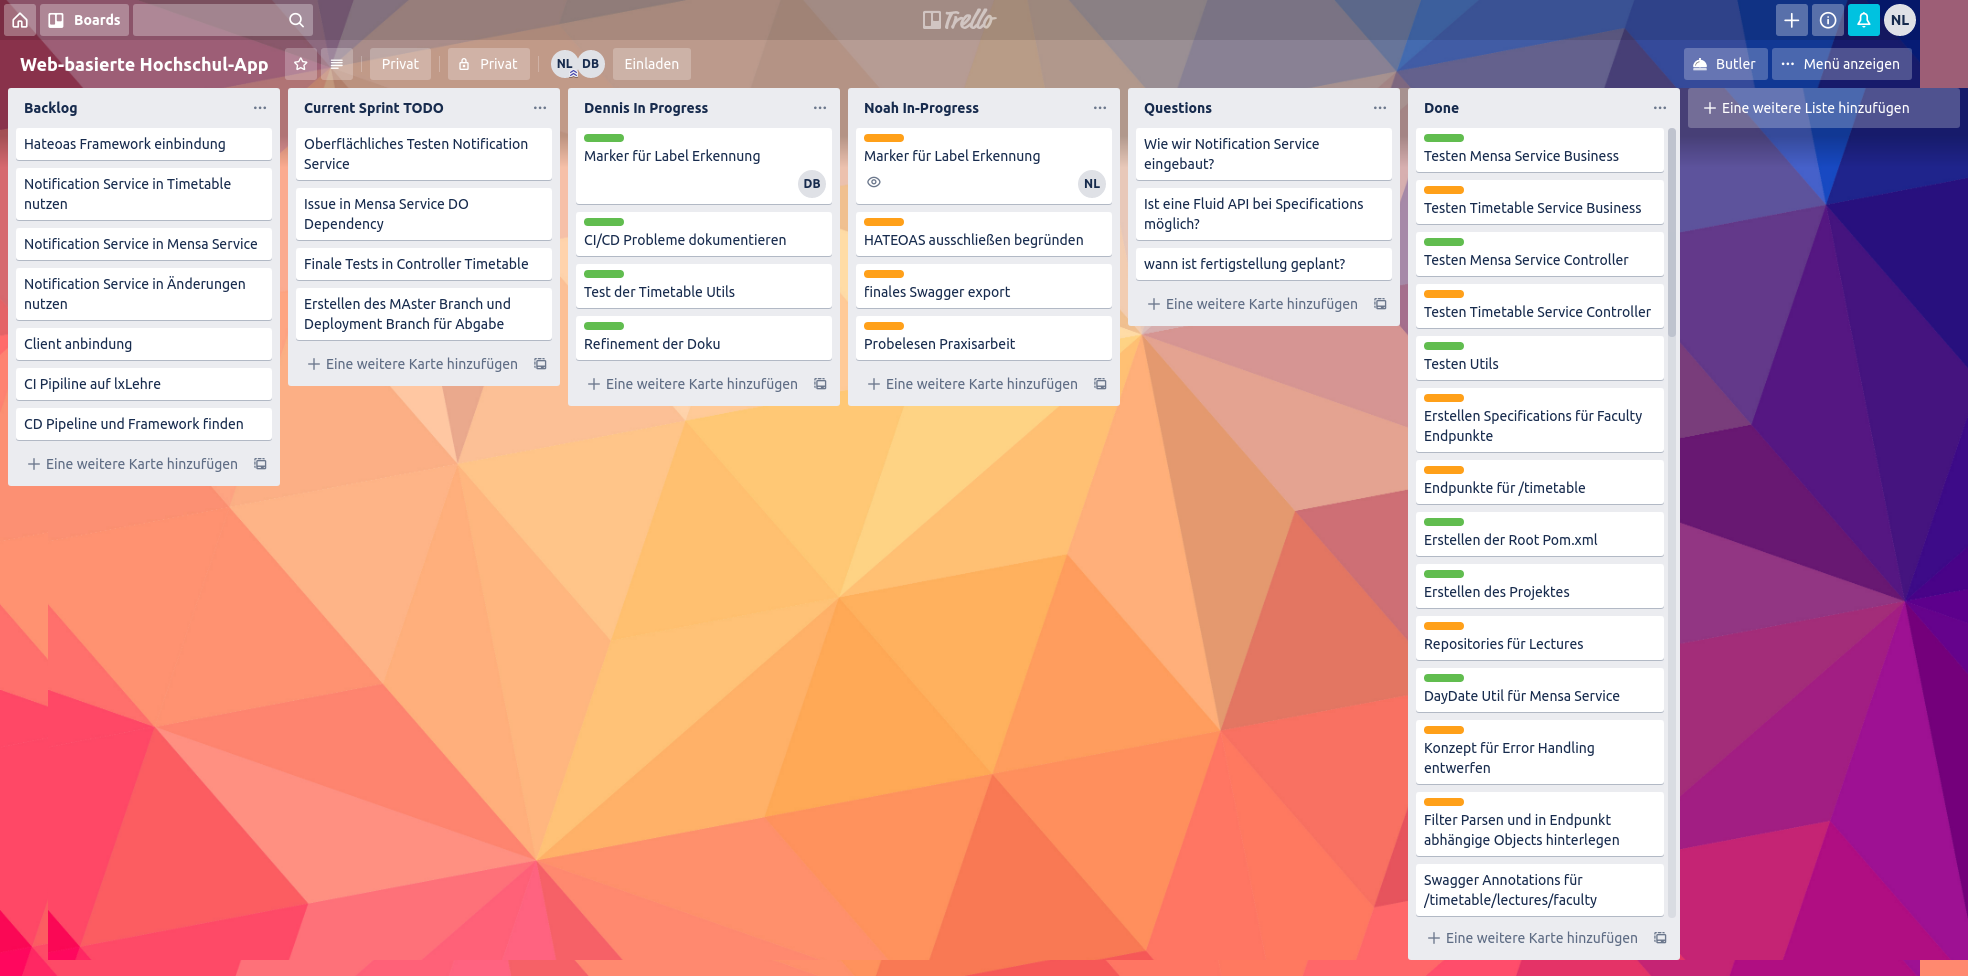
\includegraphics[width=\pictureWidth cm + 2 cm]{Bilder/Kapitel_2/trello_board.png}
\caption{Agiles Trello Board\label{fig:trello_board}}
\end{figure}

\subsection*{Sammeln der Anforderungen}

In der parallel zu dieser Arbeit erstellten Bachelorarbeit wurde bereits ein umfassendes Lastenheft erstellt, welches die funktionalen Anforderungen sammelt und kategorisiert. Anhand dieses Lastenhefts wurde ein Pflichtenheft \footnote{Siehe Anhang \ref{tab:lastenheft}} erstellt, aus dem dann die technischen Aufgaben abgeleitet wurden, welche dann in das Projekt-übergreifende Backlog übernommen werden konnten. Dieses sieht im genutzten \textit{Trello}-Board folgendermaßen aus:

\begin{figure}[H]
\centering
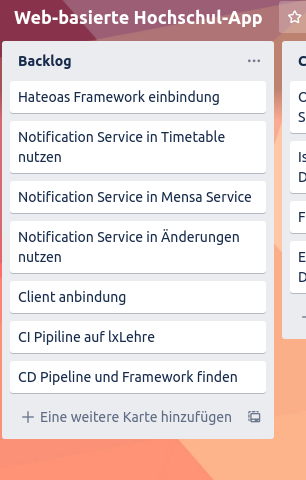
\includegraphics[width=5 cm]{Bilder/Kapitel_2/backlog.png}
\caption{Trello Board Backlog\label{fig:trello_backlog}}
\end{figure}

\subsection*{Planung eines Sprints}

Am Anfang eines jeden Sprints müssen die wichtigsten Aufgaben aus dem Backlog in das Sprint Backlog übernommen werden. Hier ist stets zu beachten, dass dabei möglichst nicht mehr Aufgaben übernommen werden, als im Sprint-Zeitraum erledigt werden können. 

\begin{figure}[H]
\centering
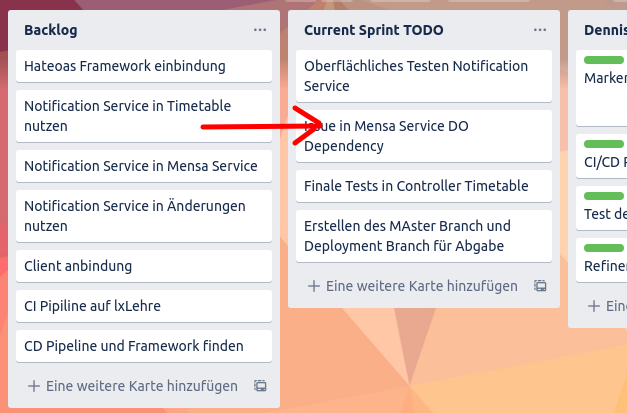
\includegraphics[width=10 cm]{Bilder/Kapitel_2/sprint_backlog.png}
\caption{Trello Board Sprint Backlog\label{fig:trello_sprint_backlog}}
\end{figure}

Innerhalb des Sprint Backlog sollte nun die Aufgaben nach ihrem Zeitaufwand bewertet werden. Die Entwickler entnehmen dem Sprint Backlog die Aufgaben geordnet nach der Priorisierung, die wichtigsten Aufgaben müssen dabei immer zuerst erledigt werden. Die Aufgaben, die am Ende eines Sprints noch nicht aus dem Sprint Backlog entnommen wurden müssen in den nächsten Sprint übernommen werden.

\subsection*{Verteilen der Aufgaben}

Wie bereits erwähnt entnehmen die Entwickler, sobald sie Zeit zur Verfügung haben, eine Aufgabe aus dem Sprint Backlog und hinterlegen sie in ihrer \textit{Todo}-Liste. Von dort aus sollten die Aufgaben mit dem entsprechenden Label versehen werden, das anzeigt, wem die Aufgabe initial zugeordnet wurde. So ist am Ende auch zu erkennen, wer welche Aufgaben erledigt hat.

\begin{figure}[H]
\centering
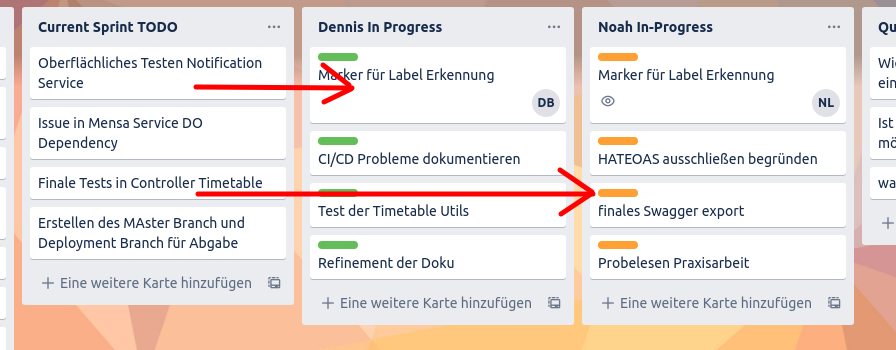
\includegraphics[width=14 cm]{Bilder/Kapitel_2/user_boards.png}
\caption{Trello Board Entwickler Todo Listen\label{fig:trello_user_boards}}
\end{figure}

Anders als im Sprint Backlog ist hierbei darauf zu achten, dass am Ende eines Sprints keine Aufgaben mehr in den Todo-Listen der Entwickler übrig sind. Diese führen sonst auf Dauer nur dazu, dass der Überblick über das Board verloren geht, was das Trello Board im Allgemeinen überflüssig machen würde. Es können allerdings jederzeit mehrere Aufgaben übernommen werden, insofern es sinnvoll ist, diese parallel zu bearbeiten.

\subsection*{Abschluss von Aufgaben}

Sobald eine der Aufgaben erledigt und getestet ist, können die Entwickler sie in die Spalte \textit{Done} übernehmen, in welcher die Aufgaben als endgültig erledigt markiert werden. 

\begin{figure}[H]
\centering
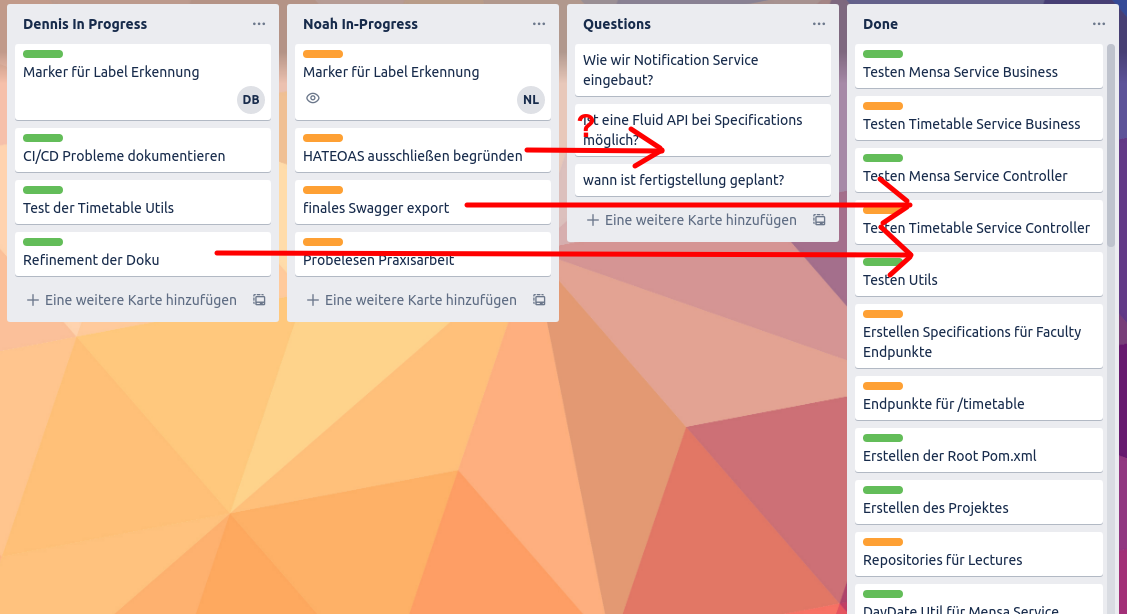
\includegraphics[width=14 cm]{Bilder/Kapitel_2/done.png}
\caption{Trello Board Liste der fertigen Aufgaben\label{fig:trello_done}}
\end{figure}

Sollten während der Bearbeitung jedoch noch Fragen auftreten, welche die Weiterarbeit oder den Abschluss der Aufgabe verhindern, so können die Fragen als einzelne Karte in die Spalte \textit{Questions} erstellt werden. Wenn die Weiterarbeit an einer Aufgabe bis zur Beantwortung der Frage nicht möglich ist, so kann man die Aufgabe auch als Ganzes in die Spalte \textit{Questions} verschieben.\\
\linebreak
Abschließend ist zur Organisation des Projektes zu sagen, dass viele Ansprüche und Konzepte, die \textit{Scrum} mit sich bringt, in einem Team von zwei Entwicklern nicht sinnvoll sind. Dennoch sollte die Grundidee aufgenommen werden, um eine Struktur in der Entwicklung beizubehalten und um wichtige Aufgaben nicht zu vergessen. Dies ist durch die abgewandelte Nutzung des \textit{Scrum}-Konzepts gelungen.
\chapter{Technologien}
\label{sec:technologien}

Es gibt verschiedene Möglichkeiten Microservices zu implementieren. Möchte man diese erschließen, sollte man mindestens zwischen vier Ebenen in der Softwarehierarchie unterscheiden. Diese sind die genutzte Programmiersprache, die verwendeten Frameworks, der Aufbau der Architektur und die genutzte Protokolle in der Kommunikation mit dem Client. Da das Service-Orientated-Design, die Schichtenarchitektur und die Nutzung von \ac{REST} in Verbindung mit \ac{HTTP} bereits in der parallel zu dieser Arbeit geschriebenen Bachelorarbeit festgelegt wurden, wird in dieser Arbeit nur noch auf die Programmiersprache und die genutzten Frameworks eingegangen\autocite[Siehe][]{dnba}.  Zusätzlich zu der verwendeten Programmiersprache können auch unterschiedliche Bibliotheks- und Quellcodeverwaltungstools zur Unterstützung genutzt werden. Die bei der Implementierung des Prototypen der neuen Hochschul-\ac{App} verwendeten Programmiersprachen, Frameworks und Hilfstools werden im folgenden genauer betrachtet.

\section{Programmiersprache}
\label{sec:programmiersprache}
%http://pypl.github.io/PYPL.html
Bei der Wahl der Programmiersprache gilt es im Allgemeinen auf folgende Punkte zu achten:

\begin{itemize}
\item Allgemeine Beliebtheit
\item Nutzbarkeit der Sprache
\item Zuverlässigkeit der Sprache
\item Eignung für Anwendung
\item Programmiererfahrung in der Sprache
\end{itemize}

Da der Prototyp der Hochschul-\ac{App} in der Zukunft von Studierenden gepflegt und weiterentwickelt wird, werden für die Auswahl der Programmiersprache nur drei Möglichkeiten in Betracht gezogen, die in den Vorlesungen der Fakultät Informatik an der Hochschule auch gelehrt werden. Diese sind \ac{JS}, \ac{PHP} und Java.

\subsection*{Kandidaten}
Für ein besseres Verständnis der folgenden Bewertungen werden die drei Programmiersprachen kurz vorgestellt.

\subsubsection*{JavaScript} 

Der Autor Christian Wenz beschreibt die anfängliche Intention der Programmiersprache JavaScript wie folgt:

\begin{quote}
%seite 18 javascript zitiert
Mit JavaScript kann man die eher beschränkten Möglichkeiten von HTML erweitern. Es handelt sich bei JavaScript um eine clientseitige Programmiersprache. Das heißt, alles läuft im Browser ab, und man muss keine besonderen Server-Voraussetzungen erfüllen\autocite[][18]{javascript}.
\end{quote}

%seite 19 javascript ref
Ursprünglich wurde \ac{JS} 1995 von Netscape für deren Internet Browser in der Version 2.0 unter dem Namen LiveScript entwickelt. LiveScript war eine Programmiersprache, die dafür gedacht war, auf \ac{HTML}-Seiten Inhalte dynamisch zu manipulieren. Da die Syntax stark an die der Programmiersprache Java angelehnt war, wurde LiveScript später aus Marketinggründen zu JavaScript umbenannt, jedoch hat die Sprache bis auf die syntaktischen
Ähnlichkeiten keine weiteren Gemeinsamkeiten mit Java\footnote{Vgl. a.a.O S. 19}.
\\
\linebreak
Heute kann man mit \ac{JS} dank Frameworks wie \textit{Node.js} oder \textit{Angular} weitaus komplexere Anwendungen schaffen. So kann man nicht nur dynamisch \ac{HTML}-Inhalte manipulieren, sondern auch Contentmanagement betreiben oder ganze Serveranwendungen implementieren. 

\subsubsection*{Hypertext Preprocessor} 

%seite 31 php ref
Ursprünglich als Hobby-Projekt des Entwicklers Rasmus Lerdorf unter dem Namen \textit{Personal Homepage Tools} entstanden, entwickelte sich \ac{PHP} zu einer Programmiersprache mit der man einfach dynamische Webanwendungen erstellen kann. Anfangs bestand \ac{PHP} nur aus einer Sammlung von \textit{Perl}-Scripten die den Zugriff auf Webseiten protokollierten. Jedoch wurde der Funktionsumfang stetig erweitert, weshalb \ac{PHP} später aus Performanz gründen komplett in der Programmiersprache \textit{C} verfasst wurde\autocite[Vgl.][31\psqq]{php}.
\\
\linebreak
Heute zeichnet sich \ac{PHP} vor allem durch seine umfangreichen Funktionsbibliotheken und durch seine hervorragenden Anknüpfungsmöglichkeiten an Datenbanksysteme aus. \ac{PHP}-Scripte liegen ständig auf dem Webserver und werden nie mit dem statischen Content an den aufrufenden Client ausgeliefert. Sie werden bei einer Anfrage des Clients auf dem Server ausgeführt und liefern danach eine Antwort zurück. Somit eignen sich die \ac{PHP}-Scripte ebenfalls als eine Implementierungsmöglichkeit für Server.

\subsubsection*{Java} 

%seite 49f java ref
Java entstand in den 1970er Jahren als Wunsch des Softwareentwicklers Bill Joy, die Vorteile einiger bereits etablierten Programmiersprachen wie \textit{C} und \textit{Mesa} in einer neuen Sprache zu vereinen. Über einige Umwege entstand letztendlich die Programmiersprache \textit{Oak} die schlussendlich 1994 den Namen Java bekam\autocite[Vgl.][49\psq]{java}.

%seite 51 java zit
\begin{quote}
Java ist eine objektorientierte Programmiersprache, die sich durch einige zentrale Eigenschaften auszeichnet. Diese machen sie universell einsetzbar und für die Industrie als robuste Programmiersprache interessant. Da Java objektorientiertes Programmieren ermöglicht, können Entwickler damit relativ einfach moderne und wiederverwertbare Softwarekomponenten entwickeln\footnote{a.a.O S. 51}.
\end{quote}

In den folgenden Kapitel werden die Programmiersprachen untereinander verglichen und auf ihre Verwendbarkeit für den Prototypen der neuen Hochschul-\ac{App} analysiert.

\subsection*{Allgemeine Beliebtheit} 

Bei der Wahl der Programmiersprache sollte unter anderem auch auf die allgemeine Beliebtheit der Sprache geachtet werden, da diese die Weiterentwicklung der Anwendung maßgeblich beeinflussen kann. Sollte eine Sprache verwendet werden, die im Trend immer schlechter bewertet wird und kaum noch genutzt wird, so könnten die Studierenden in der Zukunft das Interesse an der Weiterentwicklung der Anwendung verlieren.\\
\linebreak
Hierbei sticht vor allem die Sprache Java deutlich heraus. Laut dem \ac{PYPL} liegt Java im Gesamtvergleich aller Programmiersprachen auf Platz 2 mit etwa 19\% des Anteils der Suchen von Programmiersprachen auf der Suchplattform \textit{Google}. Doch auch \ac{JS} (Platz 3, ~8\%) und \ac{PHP} (Platz 5, ~6\%) können sich laut \ac{PYPL} durchaus als beliebt bezeichnen\autocite[][]{pypl}. Anhand der Werte ist zu erkennen, dass alle drei Sprachen grundsätzlich geeignet sind, Java hier prozentual jedoch klar besser abschneidet als \ac{JS} und \ac{PHP}.\\
\linebreak
Anzumerken ist hierbei, dass \ac{PYPL} lediglich die Suchanfragen der Stichwörter zu den Programmiersprachen auf der Suchmaschine \textit{Google} untersucht und daraus die Beliebtheit der Sprachen ableitet. \ac{PYPL} nimmt dabei an, dass eine Programmiersprache umso beliebter ist, wenn sie oft in Verbindung mit Suchanfragen im Internet zu finden ist\footnote{ebd.}. Als Messwert für die Beliebtheit einer Sprache für die Auswahl der Programmiersprache in dieser Arbeit soll dieser Wert aber genügen.

\subsection*{Nutzbarkeit der Sprache} 

Ähnlich zur Beliebtheit einer Programmiersprache bietet die Nutzbarkeit der Sprachen einen weiteren wichtigen Punkt zur Entscheidungsfindung. Unter Nutzbarkeit ist in diesem Kontext der Schreibfluss, die Einfachheit des Syntax und die vorhandene Dokumentation einer Sprache zu verstehen. Des weiteren sollten auch die nötigen Rahmenbedingungen und Vorbereitungen für die Nutzung der Sprache sowie die benötigten \acp{LOC} für das Erfüllen einer bestimmten Aufgabe betrachtet werden. Auch die Lizenzierung der Sprachen spielt bei der Nutzung in einer Hochschulumgebung eine wichtige Rolle.\\
\linebreak
Der Schreibfluss bei den Sprachen Java, \ac{JS} und \ac{PHP} unterscheidet sich nur minimal. \ac{JS} lehnt seine Syntax sogar an der von Java an. Auch \ac{PHP} orientiert sich an einer ähnlichen Syntax, störend wirkt hier lediglich das \textit{\$}-Zeichen vor den Variablen, was je nach Tastatur Layout schwieriger zu tippen ist. Den größten Schreibfluss hat man wohl bei \ac{JS}, da dort Typisierung und störende Sonderzeichen komplett wegfallen. Jedoch ist das eine rein subjektive Auffassung und kann von anderen durchaus anders eingeschätzt werden. Die Dokumentation ist bei allen Sprachen hervorragend, wobei sich hier auch Java durch seine starke Community auszeichnet.\\
\linebreak
Bei der Nutzung der Sprachen und den nötigen Rahmenbedingungen stellt sich die Sprache \ac{JS} als hervorragend dar, da für die Nutzung dieser Sprache lediglich ein Web-Browser von Nöten ist. Für Java wird hingegen eine Laufzeit- beziehungsweise eine Entwicklungsumgebung benötigt, bei \ac{PHP} ein Server mit den benötigten Installationspaketen. Das schnelle Lösen von Aufgaben mit möglichst wenigen \acp{LOC} ist die Stärke von \ac{PHP}, da die Sprache eine breite Auswahl an Bibliotheken und Funktionen bereits im Sprachumfang enthalten hat.\\
\linebreak
Bei der Lizenzierung gibt es für die Sprachen \ac{PHP} und \ac{JS} keine Probleme, für Java kann die Open-Source Implementierung OpenJDK statt der originalen Version, die unter Oracle lizenziert ist, verwendet werden. Somit fällt bei der Nutzbarkeit der Sprachen kein Kandidat aus der Auswahl heraus. Anzumerken ist, dass vor allem \ac{JS} leicht zu verwenden ist, jedoch Java hier die Grundlage für de Syntax bietet. Auch die statische Typisierung der Sprache Java macht es Entwicklern leichter, fehlerfreie Software zu schreiben.

\subsection*{Zuverlässigkeit der Sprache} 

Bei der Zuverlässigkeit einer Sprache geht es vor allem um die Fehleranfälligkeit der Software, die in dieser Sprache geschrieben wurde. Hierbei ist vorweg zu sagen, dass die meisten unerwarteten Fehler durch eine fehlende Typisierung oder durch schwer lesbare Code-Abschnitte verursacht werden. Da bei der Programmiersprache Java die statische Typisierung gegeben ist und die Syntax eindeutig ist, liegt die Sprache in dieser Kategorie klar vorne. \ac{JS} und \ac{PHP} haben hier das Problem, dass in der ursprünglichen Fassung der Sprachen eine Typisierung nicht vorgesehen war und erst später durch Zusätze versucht wurde, diese einzufügen oder zumindest die Fehleranfälligkeit dieser Sprachen durch nicht-typisierte Variablen zu minimieren. Zudem bieten beide Sprachen mehrere Möglichkeiten einfache Probleme durch unterschiedlichen Syntax zu lösen, was bei der Programmierung eventuell zu Problemen führen kann. Auch die Einschätzungen dieses Absatzes sind jedoch subjektiv und müssen nicht von jedermann akzeptiert werden.

\subsection*{Eignung für Anwendung} 

Für die Eignung der Anwendung qualifiziert sich klar die Programmiersprache Java. Es ist zwar durchaus möglich, in \ac{JS} und \ac{PHP} Web-Server zu schreiben, der Ursprung beider Sprachen liegt aber in der Manipulation von \ac{HTML}-Content. Java hingegen bietet durch Java \textit{EE} und andere Spracherweiterungen nativ die Grundlagen, Web-Server zu implementieren. Durch die Laufzeitumgebung von Java ist es auch einfach, auf Servern mit hoher Rechenkraft aufwändige Anfragen zu bearbeiten. Des weiteren bieten Drittanbieter einige Frameworks für Java, die genau auf die Bedürfnisse von Web-Anwendungen ausgelegt sind.

\subsection*{Programmiererfahrung in der Sprache} 

Als letzter Punkt soll die allgemeine Programmiererfahrung der Studierenden der Hochschule Hof betrachtet werden, denn diese ist ausschlaggebend dafür, welche Sprachen in Zukunft für die Pflege und Weiterentwicklung der Anwendung in Frage kommen. Auch hier stellt sich Java in den Vordergrund, da Java in der Fakultät Informatik als Einstieg in die Programmierung genutzt wird. Weiterführende Vorlesungen bauen dann oft auf den in der Programmiersprache Java gelernten Kenntnissen auf. Sowohl \ac{JS} und \ac{PHP} werden je nach lehrenden Dozenten zwar auch behandelt, jedoch nur selten als Hauptsprache einer Vorlesung, weshalb die Kenntnisse hier innerhalb der Studierenden stark schwankt.

\subsection*{Fazit}

Trotz der Attraktivität der Sprachen \ac{JS} und \ac{PHP} im Bereich der Web-Program\-mierung und der Nutzung im Allgemeinen fällt die Wahl der Programmiersprache für den Prototypen der neuen Hochschul-\ac{App} klar auf Java. Die Kenntnisse der Studierenden der Hochschule sowie die hohe Zuverlässigkeit der Sprache und die Eignung für den Anwendungsfall des Web-Servers überwiegen hier klar.

\section{Microservice Framework}
\label{sec:framework}

Im Bereich der Server-seitigen Programmierung in Java haben sich im Laufe der letzten Jahre einige Frameworks zur Unterstützung typischer Webanwendungen etabliert. Dabei fokussieren sich diese Frameworks im allgemeinen auf verschiedene Use-Cases, zu denen zum Beispiel leichtgewichtige Anwendungen, große Serverimplementierungen oder auch große Anwendungen, die aber wenig Daten im Hintergrund halten, gehören. Um etwas genauer auf die Wahl des Frameworks einzugehen, werden kurz einige davon aufgelistet und deren Use-Cases dargestellt.\\

\begin{itemize}
\item \textbf{Spring Boot}\\
\textit{Spring Boot} ist ein Framework, das darauf ausgerichtet ist, komplexe Strukturen in einer Web Applikation einfach erstellen zu können und die Konfigurierung der Ressourcen so einfach wie möglich zu halten. Wegen der breiten Einbindung anderer Frameworks für Dinge wie Datenbankanbindung, Discovery Services und andere Hilfsmittel bietet \textit{Spring Boot} eine gute Grundlage für die schnelle Entwicklung einer großen Anwendung. \textit{Spring Boot} ist vor allem bekannt durch seine Einsatzmöglichkeiten im Microservice Bereich in Verbindung mit \ac{REST}-\acp{API}\autocite[][]{spring_boot}.

\item \textbf{Struts}\\
\textit{Struts} ist ein open-source Framework, welches für moderne Web Anwendungen entwickelt wurde. Durch eine Plug-In Architektur soll \textit{Struts} die Einbindung anderer Bibliotheken, beziehungsweise die Entwicklung neuer Schnittstelle,n deutlich vereinfachen. Struts ist nicht zwingend für Microservices ausgelegt und kann weit mehr als nur \ac{REST}-Anwendungen unterstützen\autocite[][]{struts}.

\item \textbf{Kumuluz \ac{EE}}\\
\textit{Kumuluz \ac{EE}} ist ein open-source Microservice Framework. Im Gegensatz zu \textit{Spring Boot} legt \textit{Kumuluz \ac{EE}} seinen Fokus auf auf die Entwicklung leichtgewichtiger Web Anwendungen, wobei auch hier Schnittstellen für leichtgewichtige Erweiterungen geboten werden\autocite[][]{kumuluz}.

\item \textbf{\ac{JAX-RS}/ Jersey}\\
\textit{Jersey} ist eine Implementierung von \textit{\ac{JAX-RS}}, eine Bibliothek, welche darauf abzielt, einen Standard für die Entwicklung von Java \ac{REST} Services mit Java \ac{EE} zu bereitzustellen. Da dieser Standard so viele Funktionen wie möglich unterstützen soll, ist er sehr mächtig, im gleichen Zug allerdings auch deutlich aufwändiger in der Nutzung. Des weiteren wurde \textit{\ac{JAX-RS}} auch dafür entwickelt, sowohl den Server als auch die benötigten Clients in Java zu implementieren\autocites[][]{jaxrs}[][]{jersey}.

\end{itemize}

\subsection*{Kriterien bei der Framework Wahl}
\label{sec:kriterien_framework}

Die oben genannten Frameworks sind nur eine Auswahl der bekanntesten und der meist genutzten Frameworks für Web Anwendungen. Da hier eine große Auswahl für die Entwickler zur Verfügung steht, bedarf es eine Sammlung von Funktionen, die das endgültig gewählte Framework auch beherrschen muss. Zudem gibt es auch noch einige Kriterien, die die Frameworks erfüllen sollten. Diese Funktionen und Kriterien werden hier kurz aufgelistet und erläutert.

\begin{itemize}

\item \textbf{Startzeiten}\\
Jeder Webserver muss an mehreren Punkten in seinem Lebenszyklus auch gestoppt und gestartet werden. Ist ein Server gestoppt, so kann er seine Funktionen nicht erfüllen. Diesen Zeitraum, in der ein Server keine Anfragen bearbeiten kann, nennt man \textit{Downtime}. Im Falle des Prototypen der neuen Hochschul-\ac{App} sollte sich diese \textit{Downtime} möglichst auf die Nacht beschränken. Sollte der Server dennoch aus unerwarteten Gründen in den Hauptnutzungszeiten gestoppt werden, so ist es durchaus wichtig, wie schnell er neu gestartet werden kann. Da sich die voraussichtliche Nutzung der neuen Hoch\-schul-\ac{App} auf wenige Tausend Studierende beschränken wird ist dieses Kriterium lediglich für die Weiterentwicklung relevant, da kurze Ausfallzeiten von ein paar Minuten durchaus vertretbar sind.

\item \textbf{Erste Anfrage}\\
Jeder der oben genannten Frameworks unterstützt Caching Mechanismen, die es erlauben, Daten zwischenzuspeichern, sobald sie einmal von einem Client abgefragt wurden. Das ist vor allem bei Daten sinnvoll, die sich selten ändern, da so nicht die komplette Schichtenarchitektur bis zur Datenbank des Servers durchlaufen werden muss, um die benötigten Daten abzufragen. Jedoch werden Daten in der Regel erst im Cache abgelegt, wenn sie das erste mal abgefragt wurden. So ist die Bearbeitungszeit so einer Anfrage durchaus von Relevanz. Im Falle der Hochschul-\ac{App} ist dieses Kriterium durchaus relevant, aber nicht ausschlaggebend für die Wahl des Frameworks. Die meisten Daten können gecached werden, jedoch hält sich die allgemeine Komplexität der Datenabfrage in Grenzen, was die Bearbeitungszeit von Anfragen gering hält.

\item \textbf{Antwortzeiten bei kleinen Datenmengen}\\
Wie im Punkt \textit{Erste Anfrage} bereits erwähnt wurde, liegt bei Web Server Implementierungen der Fokus auf Antwortzeiten. Dabei muss man oft die Art der Anfrage unterscheiden. Neben der ersten Anfrage einer Ressource und der Anfrage einer Ressource aus dem Cache muss man noch zwischen den angefragten Datenmengen unterscheiden. Dabei ist es irrelevant, ob die Daten gecached sind oder nicht. Kleinere Datenmengen sollten mit minimalem Zeitversatz beantwortet werden. Das ist vor allem auch bei der Hochschul-\ac{App} wichtig, denn dort werden in der Regel nur kleinere Datenmengen abgefragt, die dann aber auch möglichst schnell auf den Endgeräten der Studierenden angezeigt werden sollen

\item \textbf{Antwortzeiten bei großen Datenmengen}\\
Im Gegensatz zu den Antwortzeiten bei kleineren Datenmengen ist diese bei größeren Datenmengen im Falle der neuen Hochschul-\ac{App} weniger relevant. Es kann zwar durchaus vorkommen, dass große Datensätze angefragt werden, das sollte aber nur bei der Einrichtung der Nutzerpräferenzen und der personalisierten Daten vorkommen. Da das pro Nutzer in der Regel nur einmal passiert, sind die Antwortzeiten bei Anfragen mit großen Datenmengen weniger relevant.

\item \textbf{Verhalten bei Hochlast}\\
Jede Web Anwendung hat sehr wahrscheinlich einen Zeitraum, in der überdurchschnittlich viele Nutzer auf sie zugreifen. In dieser Zeit ist es kritisch, die Anfragen trotz der hohen Last schnell beantworten zu können, da man sonst die Nutzer abschreckt und sich zusätzlich verwundbar für \ac{DoS} und \ac{DDoS} Angriffe macht. Bei der neuen Hochschul-\ac{App} ist davon auszugehen, dass solche Stoßzeiten früh am Tag vor der ersten planmäßigen Vorlesung und durchaus auch später am Tag vor der Mittagspause entstehen können. Trotz der geringen Gesamtnutzerzahl sollte nun darauf geachtet werden, das die Webserver der Anwendung auch unter Last nur geringe Ressourcen verbrauchen, da noch nicht klar ist, wie mächtig die darunterliegende Hardware ist.

\item \textbf{Einfachheit der Entwicklung}\\
Der wohl ausschlaggebende Punkt bei der Wahl des passenden Frameworks für den Prototypen der neuen Hochschul-\ac{App} ist die Einfachheit der Nutzung dieses Frameworks. Möchte man eine Anwendung schaffen, die im Umfeld von Studierenden, die ihr sich ihr professionelles Wissen erst aneignen, weiterentwickelt werden soll, so sollte man sich auf einfache und doch mächtige Techniken beschränken.

\end{itemize}

\subsection*{Entscheidungsfindung}

Grundsätzlich erfüllen alle der oben genannten Frameworks die Kriterien aus Kapitel \ref{sec:kriterien_framework}, besonders bei der erwartet geringen Nutzung der Anwendung aufgrund der Größe der Hochschule Hof. Dennoch erweist sich das \textit{Spring Boot} Framework besonders für die Implementierung der neuen Hochschul-\ac{App}. Die Gründe hierfür werden im folgenden kurz erläutert.

\subsubsection*{Hervorragende Dokumentation}
\textit{Spring Boot} verfügt über eine hervorragende Dokumentation. Dies zeigt sich hauptsächlich durch zwei Gründe. Der erste ist die sehr simple und umfangreiche Dokumentation, die \textit{Spring Boot} von sich aus zur Verfügung stellt. Der zweite ist die große Community, die durch die Popularität des Frameworks stetig am wachsen ist. Durch diese Community sind einige Foren entstanden, in denen viele häufig auftretende Probleme bei der Entwicklung diskutiert werden.

\subsubsection*{Kompatibilität}
\textit{Spring Boot} liefert von Haus aus eine große Liste von unterstützten Frameworks mit sich. Dazu gehören unter anderem Hibernate (eine \ac{JPA} Implementierung), Zuul (\ac{API}-Gateway) und JUnit5 (Testframework). Des weiteren ist die Einbindung anderer Frameworks durch die Nutzung von Maven \footnote{Siehe \ref{sec:build_tool}} sehr einfach gestaltet.

\subsubsection*{Abstrahierung}
Web Anwendungen sind oft voller komplexer Konzepte, speziell in Verbindung mit Java \ac{EE}. Hierbei wird oft auf komplizierte Annotations, Dependency Injection und Beans gesetzt. Die Nutzung solcher Konzepte ist grundsätzlich unterschiedlich zu der normalen Verwendung der Programmiersprache Java. Des weiteren werden diese Konzepte nur geringfügig in den Vorlesung der Fakultät Informatik der Hochschule Hof gelehrt. \textit{Spring Boot} vereinfacht die Nutzung dieser Konzepte durch die Einführung der Auto-Konfiguration und vereinfachten Annotations. Dies macht Spring sehr mächtig und dennoch leicht nutzbar für Entwickler mit beschränkter Programmiererfahrung.

\subsubsection*{Einfache Nutzung}
\textit{Spring Boot} bietet ein Web-Service an, der es Nutzern erlaubt, Projekte, die mit \textit{Spring Boot} implementiert werden sollen, über eine Webseite zu erstellen und sie dann vorkonfiguriert herunterzuladen. Dieser Service heißt \textit{Spring Initializr [sic!]}\autocite[Siehe][]{initializr}. Nach dem Herunterladen des voreingestellten Projektes können Feineinstellungen dann über sogenannte \textit{Property Files} vorgenommen werden.\\
\linebreak
Aufgrund der oben genannten Vorteile des \textit{Spring} Frameworks wird dieses zur Implementierung des Prototypen der neuen Hochschul-\ac{App} genutzt. Anzumerken ist hier auch, dass die Entwickler des Prototypen bereits Erfahrung bei der Nutzung von \textit{Spring Boot} haben, was auch in die Entscheidungsfindung eingeflossen ist. Des weiteren ist festzuhalten, dass die Anwendung prinzipiell mit allen oben genannten Frameworks gut implementiert werden kann, dennoch muss das Niveau der Programmierung von Studierenden mit in Betracht gezogen werden, weshalb \textit{Spring Boot} durch seine Einfachheit und der trotzdem enthaltenen Mächtigkeit die beste Wahl ist. Genaueres zur Konfiguration und Details zum Framework \textit{Spring Boot} wird in Kapitel \ref{sec:konfig} beschrieben.

\section{Build Management Tool}
\label{sec:build_tool}

Zur einfachen Einbindung von neuen Bibliotheken und zur Konfiguration des Build Prozesses benötigt der Prototyp der neuen Hochschul-\ac{App} ein sogenanntes Build Management Tool. Die bekanntesten Vertreter dieser Tools sind aktuell Gradle, Maven und Ant. Diese Vertreter sollen nun kurz betrachtet werden, worauf dann die Entscheidung für eines der drei Tools begründet wird.

\begin{itemize}
\item \subsection*{Ant}
%Seite 37 xtreme 
\textit{Ant} ist ein Build Management Tool das von der Apache Software Foundation entwickelt wurde. Es erlaubt seinen Nutzern, den Build Prozess einer Anwendung zu automatisieren. Zudem ist anzumerken, dass \textit{Ant} speziell für Java Anwendungen entwickelt wurde. Der große Vorteil von \textit{Ant} ist seine Erweiterbarkeit, denn man kann mit selbst entwickelten Java Tasks die Automation immer weiter verfeinern\autocite[Vgl.][37]{xtreme}.

\item \subsection*{Gradle}
Im Gegensatz zu \textit{Ant} ist \textit{Gradle} ein Build Management Tool, welches dafür entwickelt wurde, jede Art von Software zu unterstützen. \textit{Gradle} ist ein open-source Projekt, das in der \ac{JVM} Umgebung läuft. Das soll den Kennern der Sprache Java ermöglichen, Erweiterungen für \textit{Gradle} zu entwickeln.\autocite[][]{gradle}

\item \subsection*{Maven}
%Seite 457 xtreme 
\textit{Maven} ist aus dem Wunsch heraus geboren, einfach neue Funktionalitäten in einen Build-Prozess während einer Entwicklung einer Anwendung hinzuzufügen. Solche Funktionalitäten können beispielsweise Unit-Tests oder das Erfassen von Codemetriken sein. Die Anfänge von \textit{Maven} bauen auf \textit{Ant} auf. Jedoch nutzt \textit{Maven} mittlerweile \textit{Jelly} als primären Scripting-Engine. Die Stärke von \textit{Maven} ist es vor allem, mächtige \textit{Ant} Skripte mit in den Build Prozess aufzunehmen\autocite[Vgl.][457]{xtreme}. Des weiteren bietet Apache ein mächtiges Verzeichnis an, das es ermöglicht, Bibliotheken in verschiedensten Versionen per \textit{Maven Dependency} automatisiert in das Projekt mit einzubinden.

\end{itemize}

\subsection*{Entscheidungsfindung}

Für den Prototypen der neuen Hochschul-\ac{App} wird das Build Management Tool \textit{Maven} genutzt. Ein Vorteil dessen ist, das \textit{Spring Boot} in seinem \textit{Spring Initializr} das Erstellen von sowohl \textit{Maven}- als auch \textit{Gradle}-Projekten unterstützt. \textit{Maven} bietet sich aus diesen zwei Möglichkeiten deshalb an, da es unter anderem sehr leicht und intuitiv zu nutzen ist. Außerdem kann man mit \textit{Maven} sehr einfach \textit{Ant} Skripte einbinden.

\section{Versionsverwaltung Tool}
\label{sec:git}

Jedes Projekt, ob nun kollaborativ erstellt oder in Eigenarbeit geschaffen, benötigt ein Versionsverwaltung-Tool, idealerweise mit der Möglichkeit den Source Code auf externen Servern zu speichern, um Verluste durch einen Ausfall des Entwickler-Computers zu vermeiden. In der heutigen Zeit kommen dabei in der Regel nur noch zwei Kandidaten in Betracht, \textit{git} und \textit{Mercurial}. Für dieses Projekt gilt \textit{git} jedoch als einzig sinnvolle Option. Das liegt vor allem daran, dass die Hochschule einen eigenen GitLab Server besitzt, welcher es ermöglicht, Projekte, die über \textit{git} verwaltet werden, zu synchronisieren und auf dem Hochschul Server zu speichern. Des weiteren ist \textit{git} das weltweit wohl verbreitetste Versionsverwaltung-Tool. Auch der Lehrinhalt der Vorlesungen der meisten Dozenten der Hochschule Hof beinhaltet lediglich das Tool \textit{git}.

\section{API Gateway}

Wie in der parallel verfassten Bachelorarbeit bereits ausführlich erläutert wurde, besteht die Architektur der neuen Hochschul-\ac{App} aus mehreren Microservices, die die implementierten Funktionalitäten jeweils kapseln\autocite[][]{dnba}. Um dennoch eine einheitliche Anwendung zu schaffen, die nach außen nur eine Schnittstelle hat, wird ein sogenanntes \ac{API}-Gateway verwendet, das als Fassade zu den einzelnen Services dienen soll. Diese Microservices sind in folgende Funktionalitäten gekapselt:

\begin{itemize}
\item Stundenplan
\item Planänderung
\item Speiseplan
\item Benachrichtigungen
\item Sicherheit
\item Anwenderverwaltung
\item Sprachzentrum
\item Termine
\end{itemize}

Jedoch ist enthält der Umfang dieser Arbeit lediglich die Stundenplaninformationen, Stundenplanänderungen Mensadaten und den Benachrichtigungsservice. Alle anderen Services werden in einer anderen Abschlussarbeit separat entwickelt. Um die Anbindung der restlichen Services zu ermöglichen, ohne dass sich die Schnittstelle nach außen ändert, dient ebenfalls das \ac{API}-Gateway. Das Gateway ermöglicht es ebenfalls, zusätzlich zur Fassaden-Funktion, ein Load-Balancing der einzelnen Services zu konfigurieren, wenn diese redundant auf mehreren physischen Instanzen laufen. Die Auswirkung, die bei der redundanten Haltung der Service-Instanzen in Kombination mit der Microservice-Architektur anfallen würden, sind in der folgenden Abbildung bildlich dargestellt.

\begin{figure}[H]
\centering
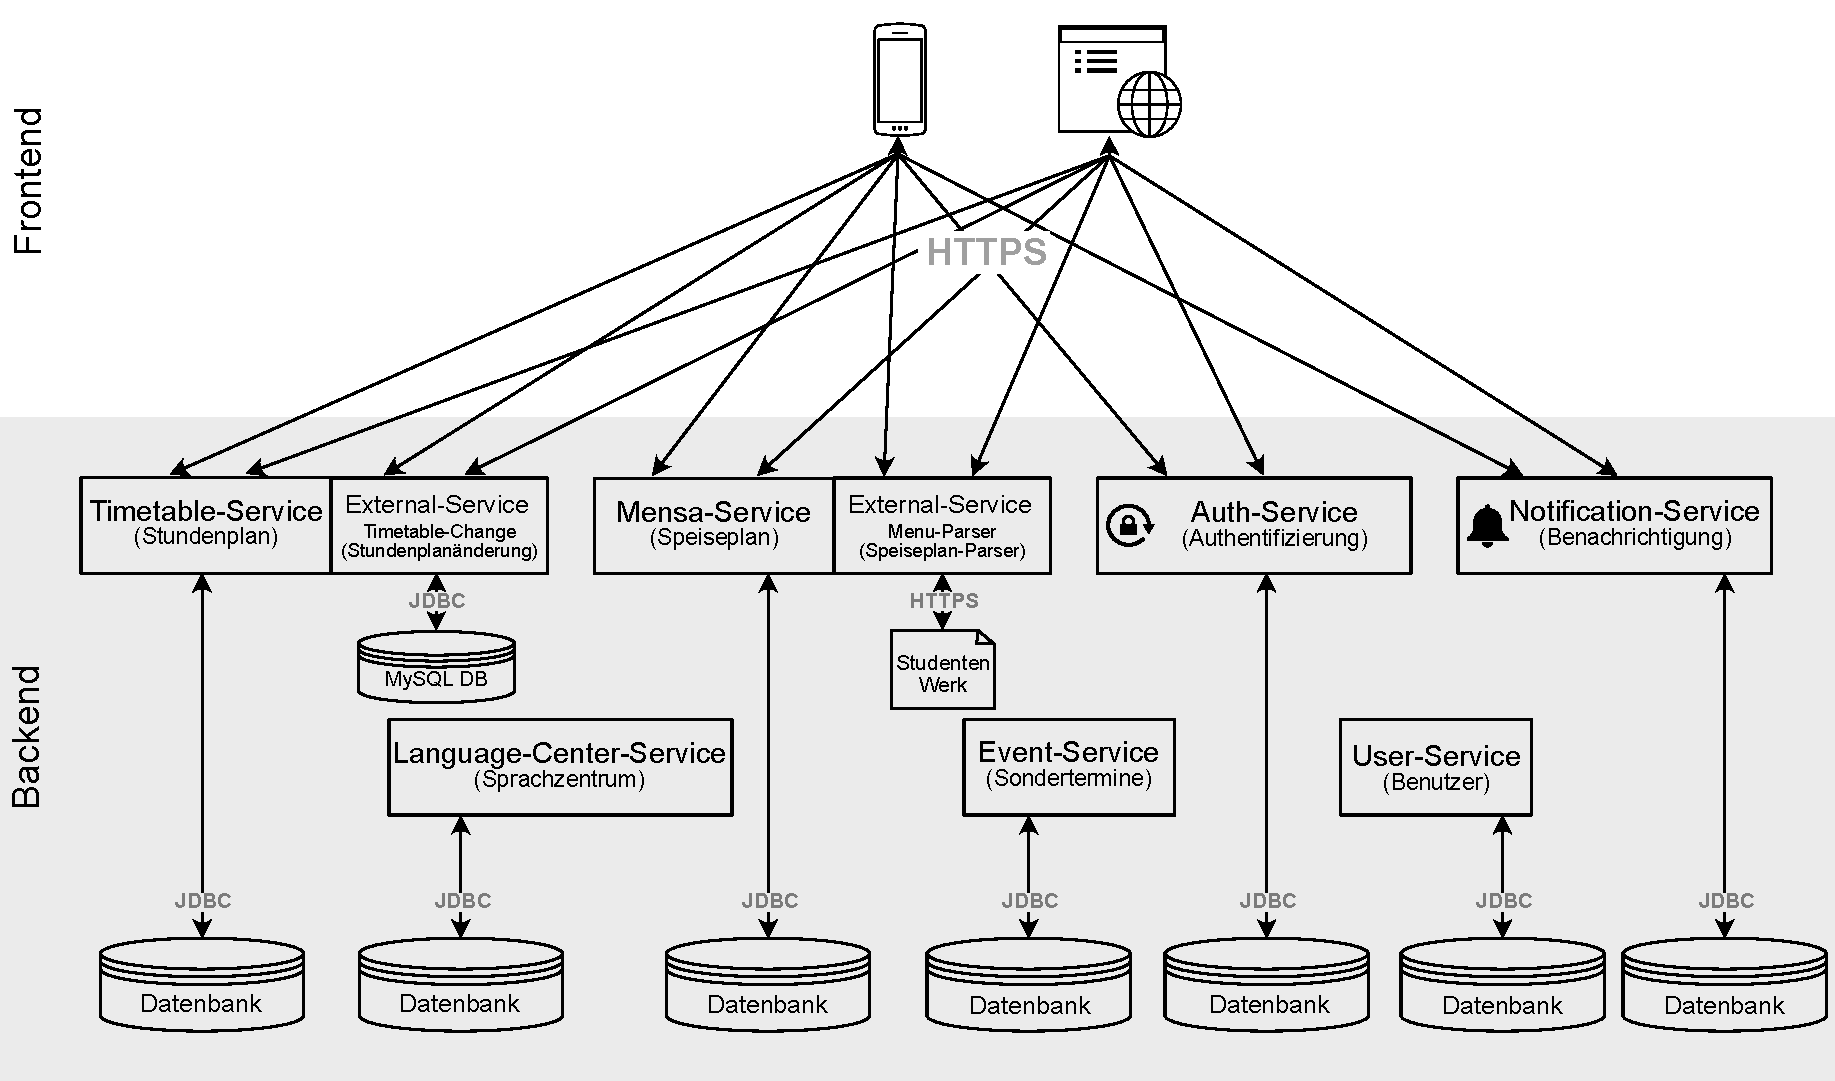
\includegraphics[width=\pictureWidth cm + 2cm]{Bilder/Kapitel_3/app_architektur_no_proxy.pdf}
\caption{Hochschull-APP Architektur ohne Gateway\label{fig:architekturnoproxy}}
\end{figure}

Eine weitere Funktion des Gateways ist die Versionsverwaltung der Services, da dieses Projekt lediglich den Prototypen implementiert und in Zukunft noch weitere Releases erscheinen werden. Deshalb und wegen der bereits genannten Vorteile wird im Prototyp ein \ac{API}-Gateway eingebunden.

\begin{figure}[H]
\centering
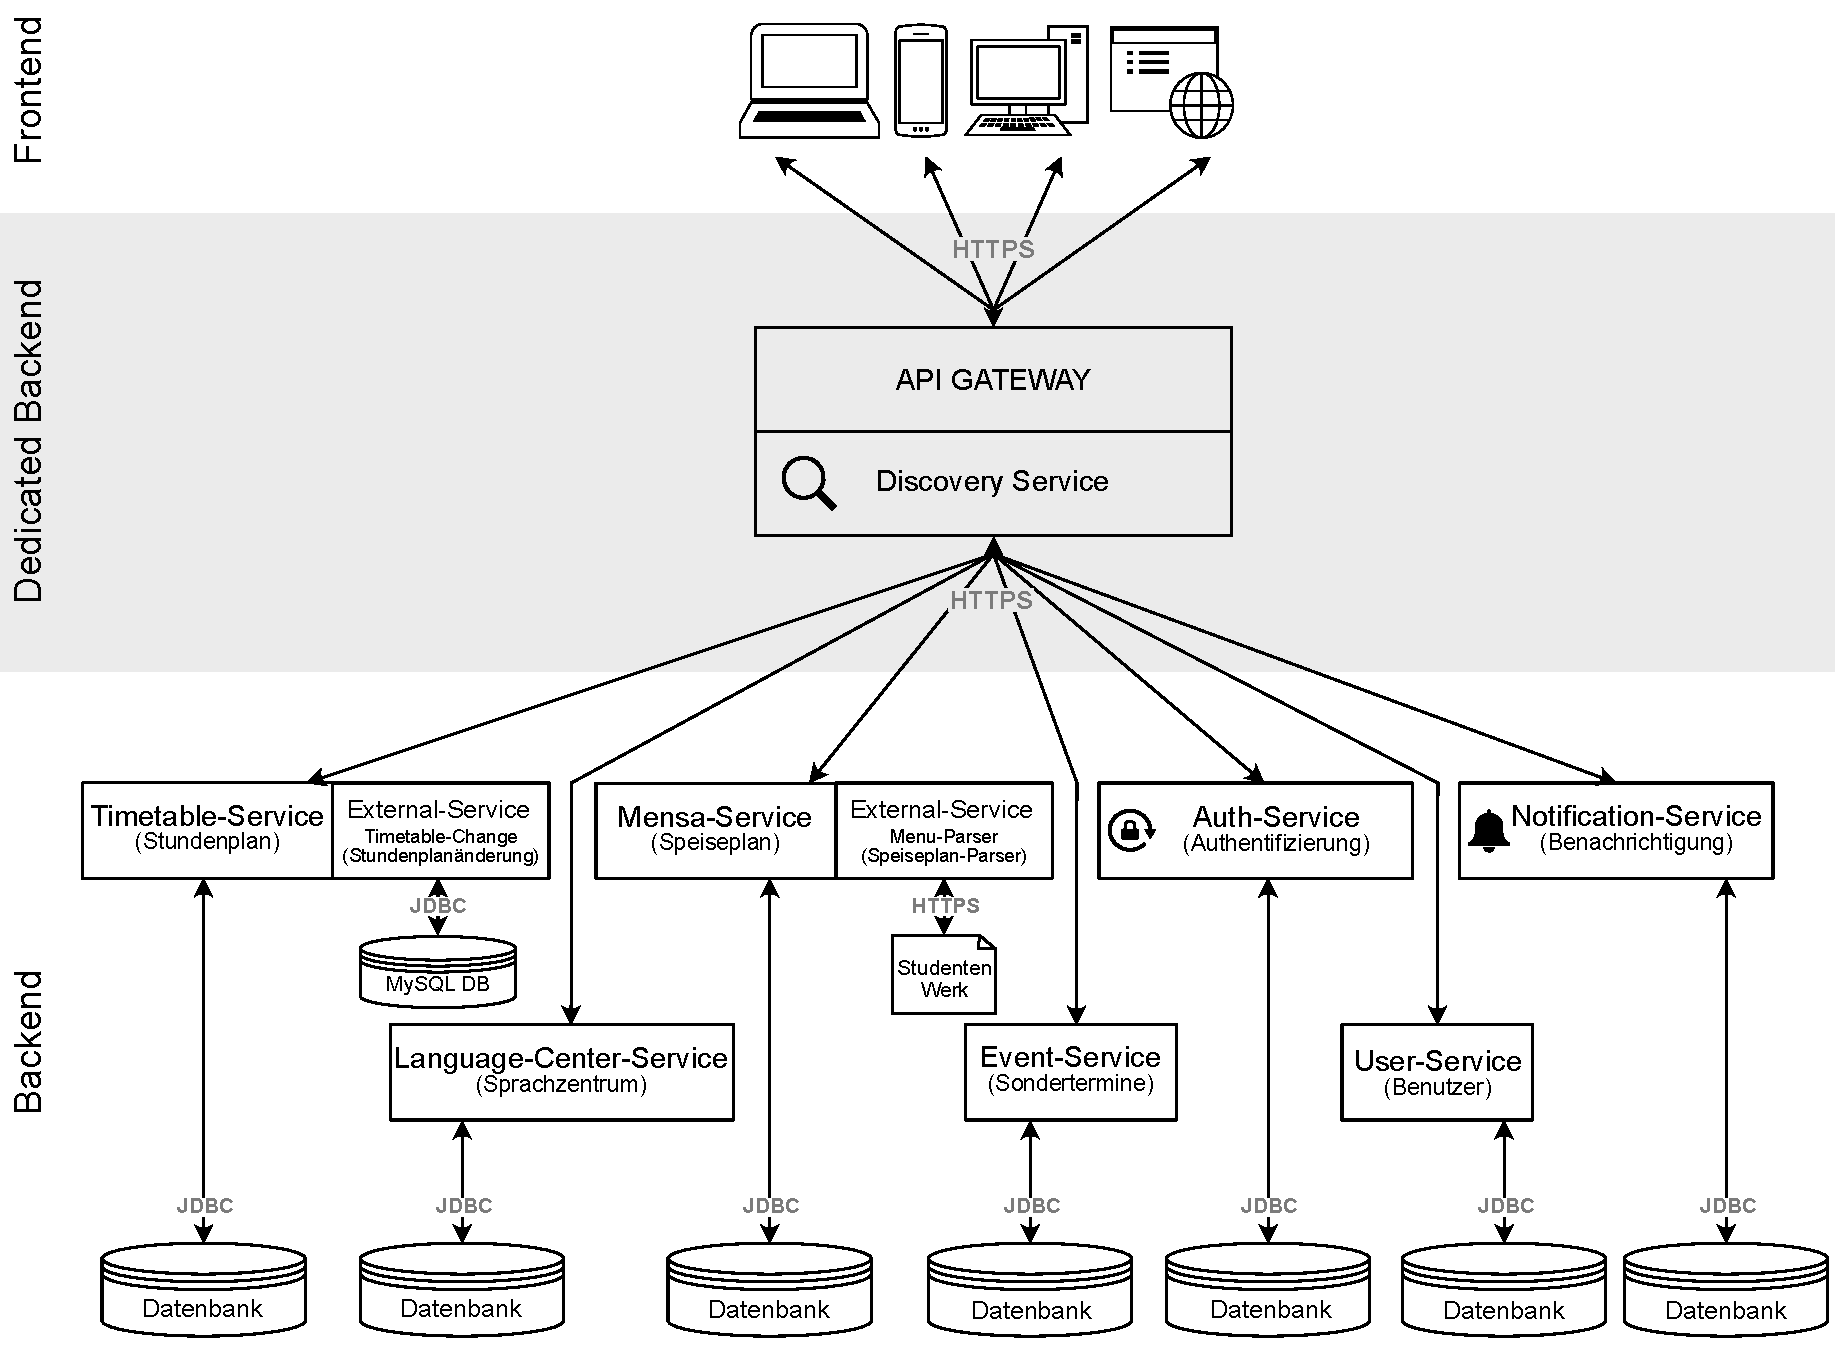
\includegraphics[width=\pictureWidth cm + 2cm]{Bilder/Kapitel_3/app_architektur_proxy.pdf}
\caption{Hochschul-APP Architektur mit Gateway\label{fig:architekturwithproxy}}
\end{figure}

Für die Implementierung des Gateways bieten sich ähnlich wie beim Microservice Framework zahlreiche Alternativen. Darunter sind unter anderen \textit{NGINX}, \textit{Spring Cloud Gateway}, \textit{Zuul} und \textit{KrakenD}. Da die Wahl des Microservice Frameworks jedoch bereits auf \textit{Spring Boot} gefallen ist, wurde die Auswahl der \ac{API}-Gateway Frameworks auf lediglich zwei Kandidaten reduziert, welche bereits in Verbindung mit \textit{Spring} getestet wurden und mit dem Framework harmonieren. Diese Frameworks sind \textit{Zuul} und \textit{Spring Cloud Gateway}.\\
\linebreak
Auch zwischen diesen beiden Frameworks bedarf es jedoch kaum eines aufwändigen Vergleichs, da die von \textit{Spring} entwickelte Gateway Implementierung auf der Basis von \textit{Zuul} implementiert wurde und dieses in Zukunft auch endgültig in Verbindung mit \textit{Spring Boot} ablösen soll. Zudem wurde der Support für \textit{Zuul} in der Version 1.0 eingestellt, was potentielle Sicherheitslücken nicht ausschließen lässt. Neuere Versionen des Frameworks werden von \textit{Spring} ohnehin nicht mehr unterstützt.

\section{Service Registrierung und Discovery}
\label{sec:registryanddiscovery}

Durch die Nutzung des \ac{API}-Gateways wurde die Auslagerung der Funktionalitäten in dezentrale Einheiten ermöglicht. Das bringt, wie bereits erwähnt, einige Vorteile mit sich, erfordert jedoch auch, dass das Gateway selbst die Adressen der einzelnen Services kennt. Diese müssen sich dadurch mit ihren physischen Adressen beim Gateway oder einer anderen zentralen Instanz registrieren. Hierfür wurde beim Prototypen der Hochschul-\ac{App} ein Discovery Server eingebaut. Dieser kümmert sich um das Load-Balancing, verteilt die Anfragen zwischen den Instanzen und leitet die Anfragen an eine ausgefallene Instanz an den passenden Backup Service weiter.\\
\linebreak
Für die konkrete Entwicklung dieser Discovery Funktion gibt es eine Reihe bewährter open-source Lösungen. Zu diesen gehören Frameworks, die auf die Konsistenz der Services ausgelegt sind, wie \textit{Apache Zookeeper}, \textit{Doozer} und \textit{Etcd}, jedoch auch Frameworks, die auf dedizierte Lösungen setzen, um sich auf Load-Balancing und die eigentliche Service Discovery zu konzentrieren, wie \textit{netflix Eureka}, \textit{Spotify DNS}, \textit{SkyDNS}, \textit{NSQ} oder \textit{SmartStack}\autocite[][]{cloud_discovery}.
% referenziert http://jasonwilder.com/blog/2014/02/04/service-discovery-in-the-cloud/
\\
\linebreak
Alle Frameworks bringen bestimmte Vor- und Nachteile mit sich, wobei für die eigentliche Implementierung der Hochschul-\ac{App} prinzipiell jedes der genannten Framework verwendet werden kann. Deshalb wird bei der Wahl des Discovery Frameworks das Hauptaugenmerk auf die Einbindung in das \textit{Spring} Framework gelegt. Speziell n der \textit{Spring Cloud} existieren bereits Lösungen für dieses Konzept, von denen eines das oben genannte \textit{Netflix Eureka} ist. Dieses baut auf Services aus dem \textit{Netflix \ac{OSS}} auf, aus dem auch einige Konzeote in \textit{Spring Cloud} genutzt werden, weshalb sich \textit{Netflix Eureka} perfekt für die Nutzung im Prototypen der neuen Hochschul-\ac{App} eignet.

\section{Benachrichtigung}
\label{sec:notification}

Da es technisch nicht möglich ist, über eine reine Datenschnittstelle Benachrichtigungen an die aufrufenden Clients zu senden, weil nie klar ist, welche Clients den Dienst nutzen, muss ein Benachrichtigungsservice genutzt werden, bei dem sich die Clients registrieren können, um über mögliche Änderungen informiert zu werden. Hierbei bieten sich in der Praxis zwei Alternativen, eine  Push-Benachrichtigungs-\ac{API} selbst entwickeln oder das Nutzen von Drittanbieter Software mit Cloud-Lös\-ungen. Da das Implementierung und Testen solcher Anwendungen sehr aufwändig ist, fällt die eigene Entwicklung dabei aus den möglichen Umsetzungen heraus\autocite[][]{webpush}.
%ref https://golb.hplar.ch/2019/08/webpush-java.html
\\
\linebreak
Deswegen wird auf eine Drittanbieter Lösung bei der Prototyp Entwicklung zurückgegriffen. Diese kümmern sich selbstständig um die Unterstützung unterschiedlicher Anwendungen und der Verschlüsselung der Benachrichtigungen. Eine weit verbreitete und mittlerweile gut getestete Lösung ist das von Google entwickelte \ac{FCM}. \ac{FCM} ermöglicht plattformübergreifende Benachrichtigungen mit der zusätzlichen Unterstützung von mobilen Endgeräten, was im Fokus der Entwicklung der neuen Hochschul-\ac{App} liegt\autocite[][]{firebase_home}. Die kostenlose Lizenz für \ac{FCM} ist für die Hochschull-\ac{App} mehr als ausreichend. Es können täglich bis zu 20.000 Benachrichtigungen mit einem Nachrichteninhalt von 4\ac{kB} an Clients versendet werden. Das entspricht um die 4096 Buchstaben pro Nachricht. Ein weiteres Argument für die Verwendung von \ac{FCM} ist die einfache Einbindung des \textit{Firebase Admin \ac{SDK}} über Maven. Dieses erlaubt die Konfiguration der Authentifizierung, Registrierung und des Versenden von Nachrichten über einen Service und über die Programmiersprache Java.

\chapter{Konfiguration}
\label{sec:konfig}

Um den Aufbau und die Einstellungen der grundlegenden Anwendung der Hoch\-schul-\ac{App} besser verstehen zu können, bietet es sich an, die Schritte, die bei der Erstellung dieser Anwendung durchgeführt worden sind, zu dokumentieren und zu erläutern. Im folgenden werden diese Schritte deshalb aufgeführt. Es soll jedoch nicht nur um die Einrichtung der Software im Allgemeinen gehen, sondern auch um die Einrichtung der Entwicklertools, die für die Arbeit an der Hochschul-\ac{App} bereitgestellt wurden.

\section{Entwicklungsumgebung}
\label{sec:entwicklungsumgebung}

Für die Arbeit am Prototypen der neuen Hochschul-\ac{App} wird das Nutzen einer \ac{IDE} empfohlen. Der Vorteil hierbei liegt in der Verwaltung der Projektstruktur, der Abhängigkeiten und der automatisierten Kompilierung des Quellcodes. Dabei ist es grundsätzlich egal, welche \ac{IDE} verwendet wird, da die meisten dieser Entwicklungsumgebungen die wichtigsten Funktionen bereits beinhalten. Dennoch wird hier explizit die Java \ac{IDE} \textit{IntelliJ IDEA} der Firma \textit{JetBrains} empfohlen\autocite[Siehe][]{intellij}. \textit{IntelliJ IDEA} wird in zwei Formaten angeboten, einer umfassenden \textit{Ultimate} Version, welche alle Funktionen der Anwendung beinhaltet, und einer vereinfachten \textit{Community} Edition, welche kostenfrei ist, jedoch nicht alle Features unterstützt. Studierende können sich kostenlos eine Lizenz für \textit{IntelliJ IDEA Ultimate} besorgen.\\
\linebreak
Im folgenden wird kurz die Einstellung der \ac{IDE} \textit{IntelliJ IDEA Ultimate} erläutert, welche nötig ist, um die Vorteile der geschaffenen Rahmenbedingungen vollständig zu nutzen. Die genutzte Version bei der Demonstration ist \textsc{IntelliJ IDEA 2019.3.1 (Ultimate Edition)}. Es wird hier noch einmal darauf hingewiesen, dass die Entwicklung unabhängig von der genutzten \ac{IDE} möglich ist, die Nutzung von \textit{Intellij IDEA} hier jedoch empfohlen wird. Außerdem soll hierbei auch noch einmal auf die Lizenzbedingungen der \textit{Ultimate} Version verwiesen werden\autocite[Siehe][]{ultimate}.

\subsection*{Hot Deploy}
\label{sec:hot_deploy}
       
\textit{Hot Deploy} ist eine Funktion, welche es ermöglicht, den Programmcode einer Software automatisiert bei der Erkennung von Änderungen oder beim manuellen Anstoßen einer Speicherung zu kompilieren und dann auf den laufenden Server zu deployen. Das erspart dem Entwickler die Wartezeit, die beim manuellen Deployment einer Serversoftware entsteht und ist bei der Entwicklerarbeit von großem Vorteil.

\subsubsection*{Einstellung in der \ac{IDE}}

Die Schritte zur Einrichtung sind folgende:

\begin{enumerate}

\item Öffnen der \ac{IDE} \textit{Intellij IDEA} und des Projektes, das die Microservices enthält
\item Öffnen des Menüpunktes \textit{File -> Settings} (Alternativ \textsc{STRG+ALT+S})
\item Auswählen der Option \textit{Build,Execution,Deployment -> Compiler}

\begin{figure}[H]
\centering
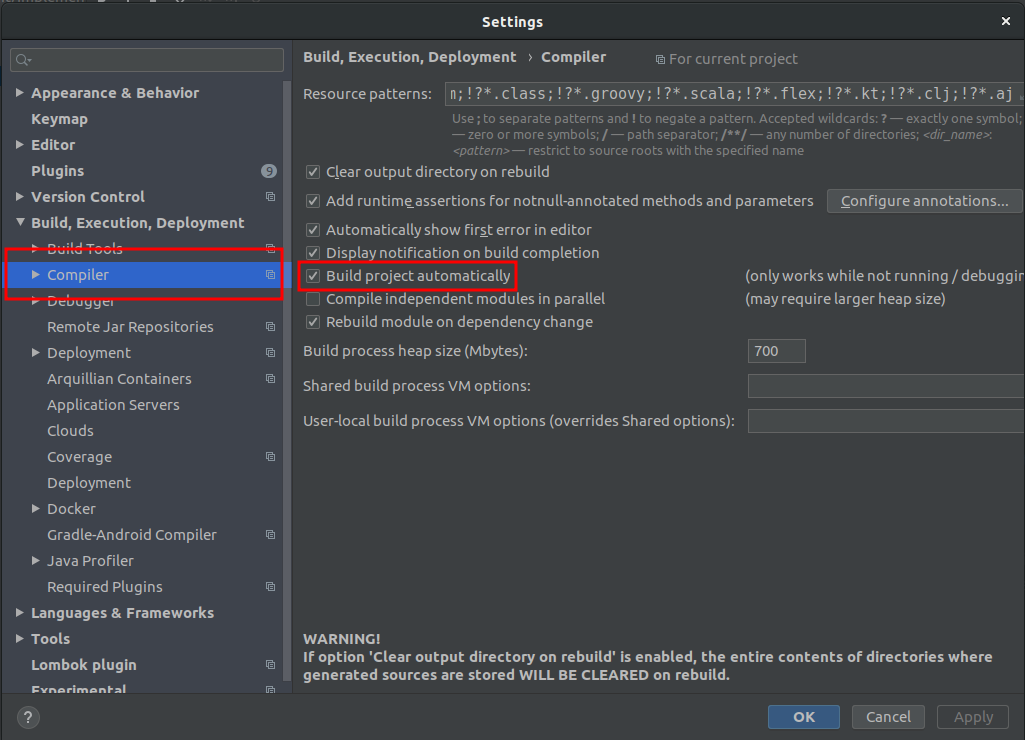
\includegraphics[width=\pictureWidth cm]{Bilder/Kapitel_4/hotdeploy.png}
\caption{Hot Deployment in \textit{IntelliJ}\label{fig:hotdeploy}}
\end{figure}

\item Bestätigen der Checkbox \textit{Build project automatically}

\item Öffnen der \textit{Registry} 

\begin{enumerate}

\item Tastenkombination \textsc{STRG+N}
\item Erweitern des Suchradius auf \textit{All}
\item Suchen nach Registry
\item Auswählen des Punktes \textit{Actions -> Registry...}
\begin{figure}[H]
\centering
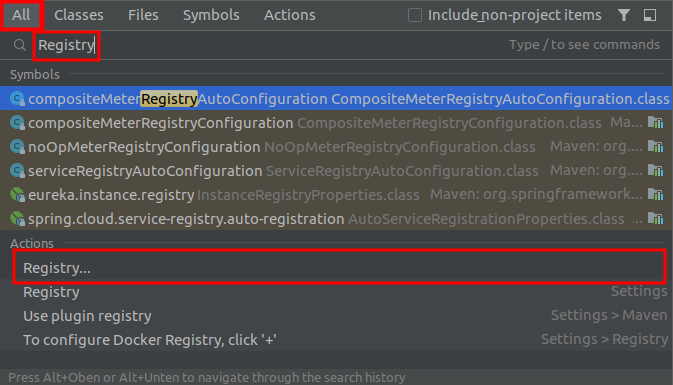
\includegraphics[width=\pictureWidth cm]{Bilder/Kapitel_4/registry.png}
\caption{Öffnen der Registry in \textit{IntelliJ}\label{fig:registry}}
\end{figure}

\end{enumerate}

\item Bestätigen der Checkbox \textit{compiler.automake.allow.when.app.running}

\begin{figure}[H]
\centering
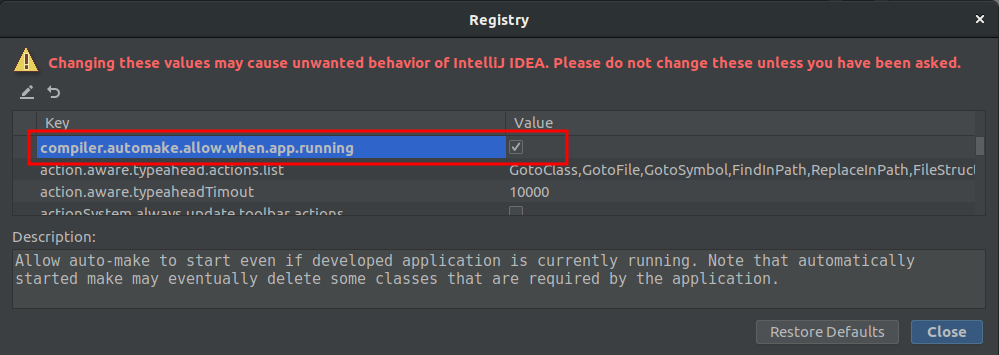
\includegraphics[width=\pictureWidth cm]{Bilder/Kapitel_4/compiler_hotdeploy.png}
\caption{Compiler Anweisung in \textit{IntelliJ}\label{fig:compiler_hotdeploy}}
\end{figure}

\item Neustart der \ac{IDE}

\end{enumerate}

Der Start der Services erfolgt nach wie vor manuell. Sobald der Service läuft, werden Änderungen automatisch in den laufenden Server übernommen.

\begin{figure}[H]
\centering

\includegraphics[width=\pictureWidth cm]{Bilder/Kapitel_4/start.png}
\caption{Start des Services in \textit{IntelliJ}\label{fig:start}}
\end{figure}

Hierbei startet der \textit{Play}-Button den Service normal, während der Button mit dem Käfer als Icon den Service im \textit{Debug}-Modus startet.

\subsubsection*{Manuelles Deployment}

Das \textit{Hot Deployment} wird in der Regel bei der Erkennung von Änderungen und in der \ac{IDE} \textit{IntelliJ IDEA} beim Drücken der Tastenkombination \textsc{STRG+S} angestoßen. Das kann auch der Fall sein, wenn gerade erst am Code geschrieben wird und die Software noch nicht kompilierbar ist. Außerdem verbraucht diese Funktion deutlich mehr Ressourcen auf dem \ac{PC} des Entwicklers, was es zu einer Funktion macht, die eventuell nicht gewünscht ist. In diesem Fall kann ein Service der Hochschul-\ac{App} folgendermaßen manuell deployed werden:

\begin{enumerate}

\item Start des Services wie in automatischem Deployment
\item Neustart des Services über Toolbar

\begin{figure}[H]
\centering
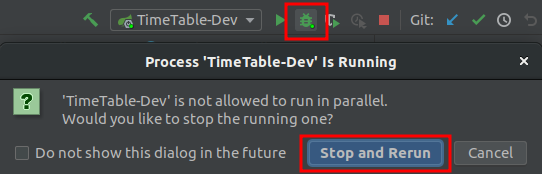
\includegraphics[width=\pictureWidth cm]{Bilder/Kapitel_4/rerun.png}
\caption{Neustart des Services in \textit{IntelliJ}\label{fig:rerun}}
\end{figure}

\end{enumerate}


\subsection*{Lombok}
\label{sec:lombok}

\textit{Lombok} ist ein Framework, welches es ermöglicht, einfachen Code, der sich in jedem \ac{POJO} befindet, nicht immer wieder neu tippen zu müssen. Durch einfache Annotations können so den \acp{POJO} \textit{Getter}, \textit{Setter}, \textit{Konstruktoren} und andere häufig verwendeten Codeabschnitte zur Kompilierzeit hinzugefügt werden. Das macht das manuelle Erstellen dieser Codeabschnitte überflüssig und macht das Projekt allgemein lesbarer, da durch die Annotations die eigentlichen Methoden-Implementierungen entfallen\autocite[][]{lombok}. Ein solches \ac{POJO} könnte nach der Nutzung von \textit{Lombok} folgendermaßen aussehen:
\newpage

\begin{lstlisting}[caption={Klassendefinition mit \textit{Lombok}}]
package test.lombok.pojo

import lombok.AllArgsConstructor;
import lombok.Getter;
import lombok.Setter;

@Getter
@Setter
@AllArgsConstructor
class POJO {
	private int attr1;
	private int attr2;    
}
\end{lstlisting}

\textit{Lombok} wird im Sourcecode des Prototypen der neuen Hochschul-\ac{App} bereits verwendet und sollte so auch in der \ac{IDE} der Entwickler konfiguriert werden, da diese sonst möglicherweise den verwendeten Sourcecode nicht kompiliert, da sie nicht erkennt, dass verwendete Methodenreferenzen von \textit{Lombok} erst zur Kompilierzeit hinzugefügt werden. Die Konfiguration in \textit{IntelliJ IDEA} erfolgt folgendermaßen:

\begin{enumerate}

\item Öffnen der \ac{IDE} \textit{Intellij IDEA} und des Projektes, das die Microservices enthält
\item Öffnen des Menüpunktes \textit{File -> Settings} (Alternativ \textsc{STRG+ALT+S})
\item Auswählen der Option \textit{Plugins}
\item Suche nach dem Plugin \textit{Lombok}

\begin{figure}[H]
\centering
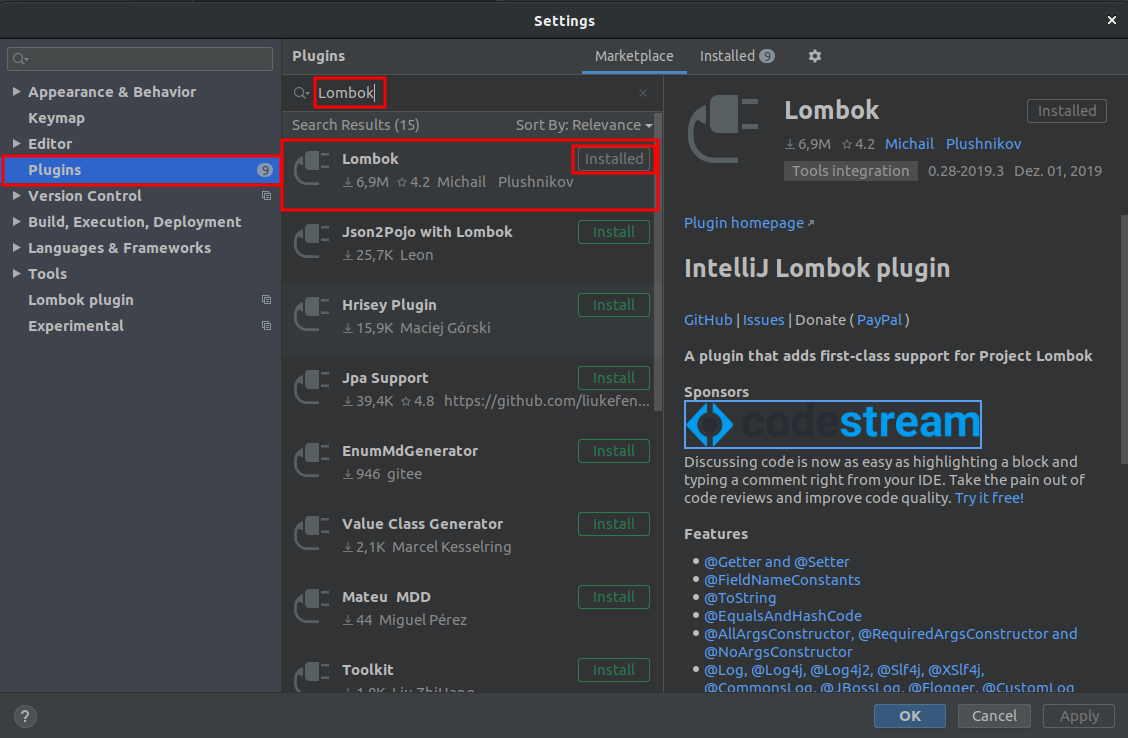
\includegraphics[width=\pictureWidth cm]{Bilder/Kapitel_4/lombok_plugin.png}
\caption{Lombok Plugin in \textit{IntelliJ}\label{fig:lombok_plugin}}
\end{figure}

\item Installation des Plugins und Neustart der \ac{IDE}

\end{enumerate}

\section{Spring Boot}
Wie bereits in Kapitel \ref{sec:framework} erwähnt wurde, wird \textit{Spring Boot} als Microservice Framework für den Prototypen der neuen Hochschul-\ac{App} verwendet. \textit{Spring} ist ein Framework, das durch die vereinfachte Einbindung anderer Bibliotheken die Entwicklung mit Java deutlich vereinfacht\autocite[Vgl.][1]{spring}. \textit{Spring Boot} zeichnet sich vor allem dadurch aus, dass es Elemente aus dem Java \ac{EE} Umfeld sowie open-source Bibliotheken zur Server-Entwicklung mit Fokus auf Microservices vereint. Im folgenden soll nun auf die Einbindung des \textit{Spring Boot} Frameworks in das Gesamtprojekt eingegangen werden.

\subsection*{Spring Initalizr}

\textit{Spring Initializr} ist ein Dienst der Entwickler des \textit{Spring} Frameworks, mit dem man voreingestellte Projekte erstellen und aus dem Dienst herunterladen kann. Dabei gibt man lediglich an, welche Abhängigkeiten das neue Projekt benötigt und mit welchen Versionen der Abhängigkeiten und Programmiersprachen das Projekt laufen soll. Durch diesen Dienst wurde ebenfalls der Prototyp der neuen Hochschul-\ac{App} erstellt, wobei hier zu beachten ist, dass alle Microservices als einzelnes Projekt betrachtet werden müssen und deshalb jeder Service seine eigenen Abhängigkeiten besitzt. Im folgenden wird kurz die Vorgehensweise zum Erstellen des Projektes erläutert, danach werden dann die einzelnen Abhängigkeiten aufgelistet.

\subsubsection*{Erstellen des Projekts}

Um ein Projekt mit \textit{Spring Initializr} zu erstellen, muss man die Website \textit{https://\-start.spring.io/} aufrufen. Danach durchläuft man folgende Schritte. Alle Abbildungen in der folgenden Abbildung stammen von der Website des Dienstes\autocite[][]{initializr}.

\begin{enumerate}

\item \textbf{Auswahl des Projekt Build Tools und Dependency Managements}\\
Für dieses Projekt wurde \textit{Maven} ausgewählt. Mehr Informationen dazu sind in Kapitel \ref{sec:build_tool} zu finden.
\begin{figure}[H]
\centering

\includegraphics[width=\pictureWidth cm]{Bilder/Kapitel_4/init_project.png}
\caption{Projektwahl in \textit{Spring Initializr}\label{fig:init_project}}
\end{figure}

\item \textbf{Wahl der Programmiersprache}\\
\textit{Spring Boot} unterstützt aktuell Java, Kotlin und Groovy. Für dieses Projekt wurde Java gewählt, zu diesem Thema wurde eine ausführliche Analyse in Kapitel \ref{sec:programmiersprache} angefertigt.
\begin{figure}[H]
\centering

\includegraphics[width=\pictureWidth cm]{Bilder/Kapitel_4/init_sprache.png}
\caption{Programmiersprachenwahl in \textit{Spring Initializr}\label{fig:init_sprache}}
\end{figure}

\item \textbf{Wahl der \textit{Spring Boot} Version}\\
Bei der Wahl der Version des Frameworks sollte man grundsätzlich eine Version wählen, die bereits aus der Snapshot Phase heraus ist. So umgeht man unvorhergesehene Fehler.
\begin{figure}[H]
\centering

\includegraphics[width=\pictureWidth cm]{Bilder/Kapitel_4/init_version.png}
\caption{Versionswahl in \textit{Spring Initializr}\label{fig:init_version}}
\end{figure}

\item \textbf{Einstellung der Projekt Metadaten}\\
\textit{Maven} Projekte erfordern der Eingabe einiger Projekt-Metadaten. Darunter fallen die \textit{Group}, welche die Organisationseinheit beschreiben soll, welche das Projekt implementiert, diverse Bezeichner für das Projekt an sich und die Version der Programmiersprache, mit der das Projekt implementiert werden soll. 
\begin{figure}[H]
\centering
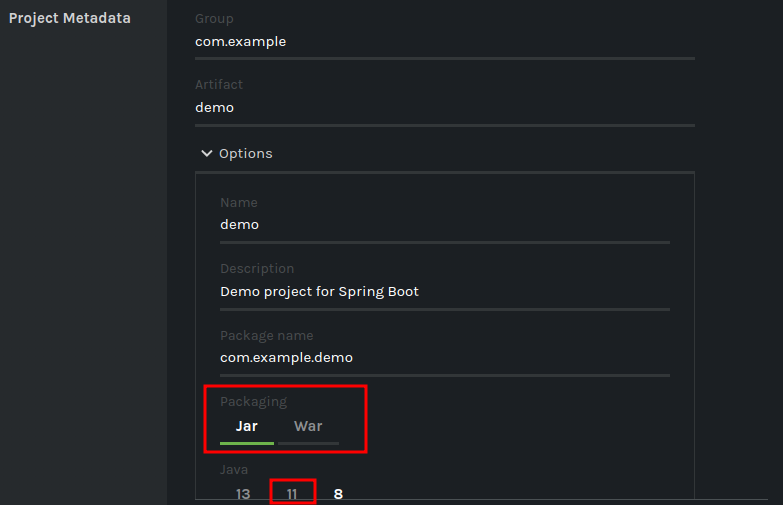
\includegraphics[width=\pictureWidth cm]{Bilder/Kapitel_4/init_meta.png}
\caption{Meta Daten in \textit{Spring Initializr}\label{fig:init_meta}}
\end{figure}

\item \textbf{Hinzufügen der benötigten Dependencies}\\
\textit{Spring Boot} unterstützt standardmäßig eine breite Auswahl an anderen Bibliotheken, welche über den \textit{Spring Initializr} einfach hinzugefügt werden können. Tut man dies über den Dient und nicht manuell mit \textit{Maven}, so vermeidet man großenteils Fehler und Konflikte in den Abhängigkeiten. Die Liste der Abhängigkeiten wird in Kapitel \ref{sec:dependencies} aufgeführt. Möchte man eine Dependency hinzufügen, so sucht man einfach im Textfeld danach und wählt diese aus. Auf der rechten Seite der Anwendung erscheint dann eine Liste aller gewählten Abhängigkeiten.
\begin{figure}[H]
\centering
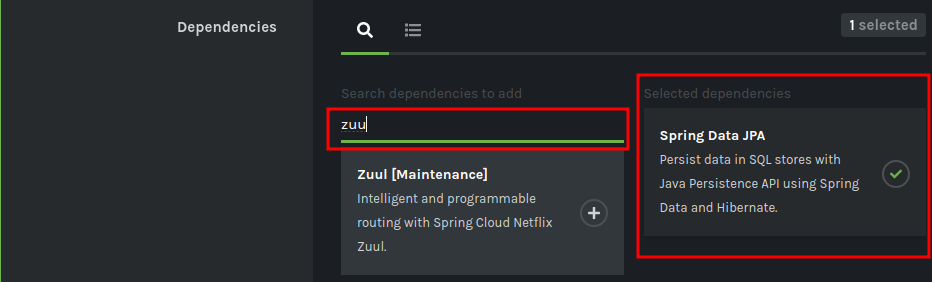
\includegraphics[width=\pictureWidth cm]{Bilder/Kapitel_4/init_dep.png}
\caption{Wahl der Abhängigkeiten in \textit{Spring Initializr}\label{fig:init_dep}}
\end{figure}

\end{enumerate}

\subsection*{Abhängigkeiten}
\label{sec:dependencies}

Da der Prototyp der neuen Hochschul-\ac{App} bereits eine breite Auswahl an Funktionen unterstützen soll und dabei auch ständig Erweiterbar und leicht zu pflegen bleiben muss, wurden in das Projekt eine Auswahl an Abhängigkeiten eingefügt. Diese werden hier nun kurz aufgelistet.

\subsubsection*{Spring Web}
Die Sammlung der vom \textit{Spring}-Framework benötigten Abhängigkeiten ist im Projekt in einer Dependency zusammengefasst. Die benötigte \textit{Maven} Dependency sieht wie folgt aus:
\begin{lstlisting}[caption={\textit{Spring Web} Dependency}]
<dependency>
    <groupId>org.springframework.boot</groupId>
    <artifactId>spring-boot-starter-web</artifactId>
</dependency>
\end{lstlisting}

\subsubsection*{JPA}
Für die Einbindung der Datenbanken wird in allen Services \ac{JPA} verwendet. \textit{Spring Boot} verwendet hierzu die \ac{JPA} Implementierung \textit{Hibernate}. Die benötigte \textit{Maven} Dependency sieht wie folgt aus:
\begin{lstlisting}[caption={Spring Data JPA Dependency}]
<dependency>
    <groupId>org.springframework.boot</groupId>
    <artifactId>spring-boot-starter-data-jpa</artifactId>
</dependency>
\end{lstlisting}

\subsubsection*{H2} 
\textit{H2} ist eine \textit{In.Memory} Datenbank, welche im Prototypen der Hochschul-\ac{App} als Testdatenbank genutzt wird, um nicht eine dauerhafte Verbindung zum Datenbank Server der Hochschule aufbauen zu müssen. Die benötigte \textit{Maven} Dependency sieht wie folgt aus:
\begin{lstlisting}[caption={H2 Dependency}]
<dependency>
    <groupId>com.h2database</groupId>
    <artifactId>h2</artifactId>
    <scope>runtime</scope>
</dependency>
\end{lstlisting}

\subsubsection*{MySQL \ac{JDBC} Dependency}
Um auf den Datenbank Server der Hochschule zuzugreifen benötigt das Projekt einen \ac{JDBC}. Da auf dem Server eine \textit{MySQL} Datenbank installiert ist wurde ein \textit{MySQL}-\ac{JDBC} eingebunden. Die benötigte \textit{Maven} Dependency für die Version des \textit{MySQL}-Servers sieht wie folgt aus:
\begin{lstlisting}[caption={\textit{MySQL} JDBC}]
<dependency>
    <groupId>mysql</groupId>
    <artifactId>mysql-connector-java</artifactId>
    <version>5.1.6</version>
</dependency>
\end{lstlisting}

\subsubsection*{DevTools}
Das in Kapitel \ref{sec:hot_deploy} erwähnte Entwicklertool \textit{Hot Deployment} benötigt ebenfalls eine Abhängigkeit, um in \textit{Spring Boot} zu funktionieren. Die benötigte \textit{Maven} Dependency sieht wie folgt aus:
\begin{lstlisting}[caption={\textit{Spring} DevTool Dependency}]
<dependency>
    <groupId>org.springframework.boot</groupId>
    <artifactId>spring-boot-devtools</artifactId>
    <scope>runtime</scope>
    <optional>true</optional>
</dependency>
\end{lstlisting}


\subsubsection*{Hypermedia}
Die \ac{HATEOAS} Funktion wurde bereits  ausführlich in der parallel zu dieser Arbeit entwickelten Bachelorarbeit erläutert\autocite[][]{dnba}. Leider konnte diese Funktion nicht in den Umfang der fertiggestellten Funktionen aufgenommen werden. Genaueres dazu wird in Kapitel \ref{sec:probleme} angesprochen. Die Dependency wird eingefügt, jedoch auskommentiert, da das Projekt ohne die Nutzung der Abhängigkeit nicht korrekt funktioniert. Die benötigte \textit{Maven} Dependency sieht wie folgt aus:
\begin{lstlisting}[caption={\ac{HATEOAS} Dependency},commentstyle=\color{red}]
<!-- UNCOMMENT ONLY IF THIS TECHNOLOGY IS IMPLEMENTED, OTHERWISE NO BUILD-->
<!--dependency>
    <groupId>org.springframework.boot</groupId>
    <artifactId>spring-boot-starter-hateoas</artifactId>
</dependency-->
\end{lstlisting}

\subsubsection*{\textit{Eureka} Client}
Die Service Discovery des Gesamtprojektes baut auf der von Netflix entwickelten \textit{Eureka}-Bibliothek auf. Um sich auf einem \textit{Eureka} Server registrieren zu können muss ein Service ebenfalls ein \textit{Eureka} Client sein. Die benötigte \textit{Maven} Dependency sieht wie folgt aus:
\begin{lstlisting}[caption={\textit{Eureka} Service Discovery Client Dependency}]
<dependency>
    <groupId>org.springframework.cloud</groupId>
    <artifactId>
        spring-cloud-starter-netflix-eureka-client
    </artifactId>
</dependency>
\end{lstlisting}

\newpage
\subsubsection*{Lombok}
Die Verwendung von \textit{Lombok} wurde in Kapitel \ref{sec:lombok} bereits ausführlich erläutert. Die benötigte \textit{Maven} Dependency sieht wie folgt aus:
\begin{lstlisting}[caption={Lombok Dependency}]
<dependency>
    <groupId>org.projectlombok</groupId>
    <artifactId>lombok</artifactId>
    <optional>true</optional>
</dependency>
\end{lstlisting}

\subsubsection*{Swagger}
Zur automatischen Generierung der Endpunkt-Dokumentation wird \textit{Spring-Fox Swagger} genutzt. Durch \textit{Swagger} kann man \ac{REST}ful Services einheitlich dokumentieren. Durch eine einfache, Menschen-lesbare Sprache, die auf \textit{yaml} beruht, können sowohl Entwickler, als auch Maschinen die Definition verstehen.
\begin{lstlisting}[caption={\textit{Swagger} Dependency}]
<dependency>
    <groupId>io.springfox</groupId>
    <artifactId>springfox-swagger2</artifactId>
    <version>2.9.2</version>
</dependency>
\end{lstlisting}
Aus der generierten Dokumentation lässt sich ebenfalls eine automatisierte Nutzeroberfläche generieren, welche zum Testen der Endpunkte genutzt werden kann. Diese Website wird automatisch in allen Services deployed und hilft den Nutzern, die Endpunkt-Dokumentation durch eine leicht verständliche Visualisierung besser zu verstehen.
\begin{lstlisting}[caption={\textit{Swagger-UI} Dependency}]
<dependency>
    <groupId>io.springfox</groupId>
    <artifactId>springfox-swagger-ui</artifactId>
    <version>2.9.2</version>
</dependency>
\end{lstlisting}

\subsubsection*{Test dependencies}
Zum testen der einzelnen Services werden mehrere Test-Frameworks benötigt. Dazu gehören unter anderem JUnit, aber auch die von \textit{Spring} eigens entwickelten Frameworks zum mocken verschiedener Abhängigkeiten. Zum Testen der Anwendung wird in Kapitel \ref{sec:test} mehr geschrieben. Die benötigten \textit{Maven} Dependencies sehen wie folgt aus:
\begin{lstlisting}[caption={Test Dependencies}]
<dependency>
    <groupId>org.springframework.boot</groupId>
    <artifactId>spring-boot-starter-test</artifactId>
    <scope>test</scope>
    <exclusions>
        <exclusion>
                <groupId>org.junit.vintage</groupId>
            <artifactId>junit-vintage-engine</artifactId>
        </exclusion>
    </exclusions>
</dependency>

<dependency>
    <groupId>org.assertj</groupId>
    <artifactId>assertj-core</artifactId>
    <scope>test</scope>
</dependency>
\end{lstlisting}

\subsubsection*{Eureka Server}
Damit der Discovery Service die Registrierungen der Services dynamisch konfigurieren und verwalten kann, muss der Discovery Service als Eureka Server fungieren. Die dafür benötigte Maven Dependency sieht wie folgt aus:
\begin{lstlisting}[caption={Eureka Server Dependencies}]
<dependency>
    <groupId>org.springframework.cloud</groupId>
    <artifactId>
        spring-cloud-starter-netflix-eureka-server
    </artifactId>
</dependency>
\end{lstlisting}

\subsubsection*{Spring Cloud Gateway}
Um die Requests der Benutzer an die registrierten Services weiterleiten zu können, benötigt der Proxy Service die Adressen der registrierten Services. Dies wird durch die Konfiguration des Spring Cloud Gateways durchgeführt. Die dafür benötigte Maven Dependency für den Proxy Service sieht wie folgt aus: 
\begin{lstlisting}[caption={Spring Cloud Gateway Dependencies}]
<dependency>
    <groupId>org.springframework.cloud</groupId>
    <artifactId>spring-cloud-starter-gateway</artifactId>
</dependency>
\end{lstlisting}

\subsubsection*{Firebase Cloud Messaging}
Um die Push Benachrichtigungen über den Notification Service versenden zu können wird die offizielle \textit{Firebase Admid \ac{SDK}} eingebunden. Dies wurde bereits in Kapitel \ref{sec:notification} erwähnt. Die dafür benötigte Maven Dependency für den Notification Service sieht wie folgt aus: 
\begin{lstlisting}[caption={FCM Dependencies}]
<dependency>
    <groupId>com.google.firebase</groupId>
    <artifactId>firebase-admin</artifactId>
    <version>6.11.0</version>
</dependency>
\end{lstlisting}

\subsection*{Wichtige Annotations}
\label{sec:annotations}

Eine der Eigenschaften, die \textit{Spring Boot} auszeichnet, ist seine Fähigkeit, komplexe Zusammenhänge und Techniken, die ihren Ursprung im Java \ac{EE} Umfeld haben, zu abstrahieren und dem Nutzer eine gut verständliche, leicht lesbare Lösung zu bieten. Das Konzept, auf das \textit{Spring Boot} dabei verstärkt setzt sind aussagekräftige Annotations. Bereits bei der Initialisierung eines Services müssen einige Voreinstellungen durch Annotations durchgeführt werden. Diese werden im Zusammenhang mit ihrer Positionierung im folgenden kurz erläutert.

\subsubsection*{Anwendungseinstieg}

Die Wurzel eines jeden \textit{Spring Boot} Programms ist die Klasse, welche die \textsc{main}-Methode als Einstieg definiert. Diese Klasse wird in allen \textit{Spring} Anwendungen mit der Annotation \textsc{@SpringBootApplication} gekennzeichnet. Zusätzlich wird diese Klasse in den funktionalen Microservices des Prototypen der neuen Hochschul-\ac{App} mit der Annotation \textsc{@EnableEurekaClient} gekennzeichnet. Das bewirkt, dass diese Services sich bei dem in den Konfigurationen definierten \textit{Eureka}-Server als Clients registrieren.\\
\linebreak
Einige Services benötigen ebenfalls Jobs, welche in bestimmten Zeitintervallen ihre Funktionalitäten ausführen. Diese Jobs nennt man \textit{Scheduled Jobs}. Beispiele hierfür sind der \textit{Timetable-Service}, welcher ständig prüft, ob in seiner Datenquelle neue Kurse oder Änderungen eingetragen wurden und der \textit{Mensa-Service}, welcher in festen Abständen die neuen Speisepläne aus seiner Datenquelle zieht. \\
\linebreak
Die Einstiegsklasse sieht damit in der Regel folgendermaßen aus:

\begin{lstlisting}[caption={Spring Application Klasse}]
@EnableEurekaClient
@SpringBootApplication
@EnableScheduling
public class TestServiceApplication{
    public static void main(String[] args) {
        SpringApplication.run(TestServiceApplication.class, args);
    }
} 
\end{lstlisting}

\subsubsection*{Controller}

Die Klassen, die die Endpunkte verwalten und die Anfragen an die Services bearbeiten heißen in \textit{Spring} \textsc{Controller}. Um der Autokonfiguration von \textit{Spring Boot} zu symbolisieren, dass eine Klasse ein Controller ist, benötigt sie die Annotation \textsc{@RestController}. Damit der Service den \ac{URL}-Pfad einer Anfrage zu einer solchen Klasse zuordnen kann, wird die Annotation \textsc{@RequestMapping([PFAD])} benötigt. Diese Klassen benötigen in der Regel noch Property Objekte, an die sie die eigentliche Bearbeitung der Anfrage delegieren können. Diese Klassen befinden sich in der Service-Schicht, enthalten die Business Logik und heißen dementsprechend Service Klassen. Damit \textit{Spring Boot} diese Objekte als Java-Bean zur per Dependency Injection zur Verfügung stellen kann, müssen die privaten Instanzen mit der Annotation \textsc{@Autowired} versehen werden. Eine entsprechende Controller Klasse sieht dann folgendermaßen aus:

\newpage
\begin{lstlisting}[caption={Spring Controller Klasse}]
@RestController
@RequestMapping("/test")
public class TestController {

    private final Service service;

    @Autowired
    public TestController(Service service){
        this.service = service;
    }
} 
\end{lstlisting}

\subsubsection*{Service}

Die Business Logik der \textit{Spring}-Anwendung liegt in der Regel in sogenannten \textit{Service}-Klassen. Das ist auch in sämtlichen Microservices des Prototypen der neuen Hochschul-\ac{App} der Fall. Damit das \textit{Spring}-Framework diese Klassen erkennt und als Beans für die Controller zur Verfügung stellen kann müssen sie mit der Annotation \textsc{@Service} markiert werden. Des weiteren benötigen diese Klassen, ähnlich wie die Controller Klasse, eine Instanz der Klasse aus der unter der Service-Schicht liegenden Persistenz-Klasse. Im Falle der Hochschul-\c{App} wird \ac{JPA} verwendet, weshalb lediglich ein Verweis auf die benötigten \acp{DAO} der Entity Klassen injiziert werden muss. Das geschieht wiederum mit der Annotation \textsc{@Autowired}. Die Service Klassen sehen in den Hochschul-\ac{App} Microservices in der Regel wie folgt aus:

\begin{lstlisting}[caption={Spring Service Klasse}]
@Service
public class TestServiceImpl implements TestService{

    private final TestDAO dao;

    @Autowired
    public TestServiceImpl(TestDAO dao){
        this.dao = dao;
    }
} 
\end{lstlisting}

\subsubsection*{JPA}

Die Tabellen, die in den Datenbanken der neuen Hochschul-Anwendung benötigt werden, werden bei der Verwendung von \ac{JPA} als \ac{POJO}-Klassen definiert, die man auch als \textit{Business Entity} oder \textit{DataObject} bezeichnet. Passend dazu müssen solche Klassen, um von \ac{JPA} als Tabelle kannt zu werden, mit der Annotation \textsc{@Entity} markiert werden. Die Annotation \textsc{@Table(name=[Table_Name])} legt dabei den Namen der Tabelle fest, die \ac{JPA} in der Datenbank anlegen - oder falls schon vorhanden - verwenden soll. Jede Klasse, die als \textit{Entity} markiert wurde, muss ein Klassenattribut besitzen, welches mit \textsc{@Id} annotiert wird. Alle Attribute der Klasse können zudem mit \textsc{@Column(name=[Column_Name])} markiert werden, was den Spaltennamen des Attributs in der Datenbanktabelle festlegt. Des weiteren können komplexere Beziehungen mit anderen Annotations festgelegt werden. Diese können in der Dokumentation der \ac{JPA} Schnittstelle nachgelesen werden\autocite[][]{jpa_oracle}. Solche Entity Klassen können wie folgt aussehen:

\begin{lstlisting}[caption={Spring Entity Klasse}]
@Entity
@Table(name="T_TEST_ENTITY")
@Getter
@Setter
@NoArgsConstructor
@AllArgsConstructor
public class TestEntity{

    @Id
    @Column(name="TEST_ID")
    private Long id;

    @Column(name="VALUE")
    private String value;
    
} 
\end{lstlisting}

\subsubsection*{Sonstige}

Wie bereits erwähnt zeichnet sich das \textit{Spring}-Framework besonders durch seine starke Abstraktion komplexer Zusammenhänge aus. Dabei kann man zwar alle Zusammenhänge klassisch über Konfigurationsdateien - in der Regel \ac{XML} oder Property-Files - definieren, jedoch liegt die Stärke des Frameworks besonders in der annotationsbasierten Konfiguration. Zusätzliche Features, wie das \textit{Swagger}-Framework, können in der Applikationsklasse per Annotation aktiviert werden. Ein Beispiel hierfür ist die erwähnte \textit{Swagger} Annotation \textsc{@EnableSwagger2}. Weitere funktionstragende Klassen, welche als Java Bean in die Applikation eingebunden werden sollen, werden ebenfalls annotiert. Beispiele hierfür sind \textsc{@Component} und \textsc{@Configuration}. 

\subsection*{Ressourcen}
\label{sec:resources}

In \textit{Spring Boot} gibt es, wie bereits erwähnt, mehrere Möglichkeiten, die Anwendung zu konfigurieren. Dabei wird im Prototypen der neuen Hochschul-\ac{App} großenteils die annotationsbasierte Konfiguration verwendet. Dennoch gibt es einige Einstellungen, welche sich am einfachsten durch sogenannte Property Files einrichten lassen. Diese müssen für jeden Microservice einzeln angelegt werden und liegen in den Ressourcen der Anwendung. Sie werden standardmäßig \textit{application.properties} benannt und enthalten in den Microservices der Hochschul-Anwendung mindestens folgende Einstellungen:

\begin{itemize}
\item \textbf{Name}\\
Unter dieser Eigenschaft wird der Name des Services festgelegt. Dieser ist vor allem bei der Registrierung beim Eureka Server und beim \ac{API}-Gateway wichtig. Der vollständige Name der Property lautet \textsc{spring.application.name}.
\item \textbf{Port}\\
Diese Eigenschaft legt den Port fest, auf dem der embedded \textit{Tomcat}-Server, der den Microservice hostet, hören soll. Der vollständige Name der Property lautet \textsc{server.port}.
\item \textbf{Eureka-Konfiguration}\\
Für die Registrierung des Eureka Clients beim Server müssen einige Einstellungen definiert werden. Die wichtigsten werden im Beispiel \ref{code:properties} gezeigt.
\item \textbf{Log}\\
Bei einer Anwendung kann es oft sinnvll sein, wichtige Ereignisse zu loggen. Damit diese im Nachhinein abgespeichert und ausgewertet werden können, gibt es dazu eine Sammlung von Properties. Die wichtigsten werden im Beispiel \ref{code:properties} gezeigt.
\item \textbf{Datenbankverbindung}\\
Um eine Verbindung zu den Datenbank Servern aufbauen zu können, benötigt \textit{Spring Boot} eine Reihe von Informationen. Diese beschreiben in der Regel die logische Adresse des Servers, den Nutzernamen, den die Anwendung als Datenbanknutzer zugewiesen bekommen hat und das passende Passwort für diese Verbindung. Des weiteren benötigt die Anwendung dann noch Details zum Namen der genauen Datenbank, mit der sie sich verbinden soll, die Art der Installation des Servers und eventuell auch Informationen dazu, wie sich \ac{JPA} bei einer Verbindung mit dem Datenbank Server verhalten soll. Da es hierbei zahlreiche Einstellungsmöglichkeiten gibt und in einer Properties-Datei mehrere Datenbanken eingebunden werden können, wird im Beispiel \ref{code:properties} exemplarisch die Datenbank des \textit{Lx-Lehre} Servers eingebuunden. Hierbei wurden sensible Daten jedoch anonymisiert. 
\end{itemize}

Das folgende Beispiel orientiert sich an den Einstellungen in den \textit{application.properties} des \textit{Timetable}-Microservices. Hierbei wurden aus Gründen des Leseflusses allerdings nicht alle Properties aufgenommen. Die sensiblen und sicherheitstechnisch relevanten Attribute wurden anonymisiert.

\begin{lstlisting}[caption={Typische \textit{application.properties} Datei}, label={code:properties}]
spring.application.name=timetable-service
server.port=8080

eureka.client.register-with-eureka=true
eureka.client.fetchRegistry=true
eureka.client.serviceUrl.defaultZone=
	http://localhost:8081/eureka/

logging.level.org.springframework.web=WARN
logging.level.org.hibernate=ERROR
logging.file.name = ./logs/timetable-service.log

spring.datasource.lx-lehre.jdbc-url=
	jdbc:mysql://localhost:60012/default_database
spring.datasource.lx-lehre.username=default_user
spring.datasource.lx-lehre.password=5AF3_PA55W0RD
spring.datasource.lx-lehre.driver-class-name=
	com.mysql.jdbc.Driver
spring.datasource.lx-lehre.jpa.hibernate.hbm2ddl.auto=none
spring.datasource.lx-lehre.jpa.show-sql=true
\end{lstlisting}

\section{Spring Cloud Gateway}

Das Framework \textit{Spring Cloud Gateway} basiert auf den Frameworks \textit{Spring 5}, \textit{Project Reactor} und \textit{Spring Boot 2.0} und bietet eine breite Auswahl an Einstellungsmöglichkeiten. Es können Filter und Routen für spezielle Anfragen definiert werden, Discovery Clients eingebunden werden, Verschlüsselungen konfiguriert und \ac{CORS}-Einstellungen definiert werden. Von all diesen Funktionen ist für den Prototypen der neuen Hochschul-\ac{App} jedoch nur die Konfiguration von \ac{CORS} und Routen zu den Microservices relevant.

\subsection*{Routen Konfiguration}

Um die Anfragen der Clients an die richtigen Microserviecs weiterleiten zu können, müssen für jeden Client Routen definiert werden. Hierfür bietet das \textit{Spring Cloud Gateway}-Framework zwei Möglichkeiten.\\
\linebreak
\textbf{Möglichkeit 1}: Statische Routen Definition über Property- oder \ac{YAML}-Files. 

\begin{lstlisting}[caption={Gateway \textit{application.yml} Datei}, label={code:ymlgateway}]
spring:
  cloud:
    gateway:
      routes:
      - id: mensa-service
        uri: lb://MENSA-SERVICE
     	- Path=/api/mensa-service/v1/**
        filters:
        - RewritePath=/api/mensa-service/v1/(?<resource>.*), /${resource}
\end{lstlisting}

Die se Möglickeit ist vor allem sinnvoll, wenn nur wenige Routen definiert werden müssen, die sich nicht ändern. Für komplexere Konfigurationen eignet sie sich jedoch nicht. Deshalb wurde im Prototypen der Hochschul-\ac{App} die sogenannte \textit{Fluent-\ac{API}} verwendet.\\
\linebreak
\textbf{Möglichkeit 2}: Dynamische Routen-Definition (Fluent-\ac{API}) über die Einbindung eines Beans vom Typ \textsc{RouteLocator}. Die Einbindung dieser Bean kann in der \textit{Spring} Application Klasse erfolgen, da es sich aber um eine Konfiguration handelt wurde der \textit{Best Practice} Vorsatz einer \textsc{@Configuration}-Klasse genutzt.

\begin{lstlisting}[caption={Gateway Routen Konfiguration Klasse}, label={code:configgateway}]
@Configuration
public class RouteConfig {

    @Bean
    public RouteLocator proxyRoutes(RouteLocatorBuilder routeLocatorBuilder){
        return routeLocatorBuilder.routes()
            .route(route -> route.path("/api/mensa-service/v1/**")
                .filters(filter -> filter
                    .rewritePath(
                     "/api/mensa-service/v1/(?<resource>.*)", 
                     "/${resource}"))
                .uri("lb://MENSA-SERVICE")
                .id("mensa-service"))
            .build();
\end{lstlisting}

Hierbei zu beachten ist die eingebundene \ac{URL} in den Codebeispielen \ref{code:ymlgateway} und \ref{code:configgateway}. Hier werden die Vorteile des Eureka Servers voll ausgenutzt. Hierfür wird in der \textit{application-properties} lediglich der Pfad zum Eureka Server eingetragen, worauf das \textit{Spring Cloud Gateway}-Framework die benötigten Servicepfade selbstständig beziehen kann.

\subsection*{Cross-Origin-Filter Konfiguration}

Da die \ac{REST}-Schnittstelle und die Clients dieser \ac{API} meist auf unterschiedlichen Quellen laufen und viele Clients ihre Anfragen über einen Browser durch \ac{CORS} realisieren, scheitern jegliche Anfragen in der Regel an mangelnden Einstellungen zur Sicherheit bei der Nutzung mit \ac{CORS}. Da diese anfällig für Angriffe sind, blockieren die gängigen Browser solche Anfragen in der Regel. Deshalb muss das \ac{CORS} im \ac{API}-Gateway uzerst konfiguriert werden, dies erfolgt wie auch bei den Routen entweder über die Poperties- oder \ac{YAML}-Files oder über die Bereitstellung von Configuration-Beans. Die bereitgestellte BEan muss zusätzlich zur \textsc{@Configuration} Annotation noch mit \textsc{@EnableWebFlux} markiert werden. \textit{WebFlux} ist ein Framework von \textit{Spring} und bietet eine reaktive Programmierunterstützung für Webanwendungen.

\newpage
\begin{lstlisting}[caption={CORS-Filter Konfigurationsklasse}, label={code:cors}]
@Configuration
@EnableWebFlux
public class CORSFilterConfig implements WebFluxConfigurer {

    @Bean
    public CorsWebFilter corsWebFilter() {
        CorsConfiguration corsConfiguration = new CorsConfiguration();
        corsConfiguration.addAllowedMethod("*");
        corsConfiguration.addAllowedOrigin("*");
        corsConfiguration.addAllowedHeader("*");
        corsConfiguration.setAllowCredentials(true);

        UrlBasedCorsConfigurationSource urlBasedCorsConfigurationSource = new UrlBasedCorsConfigurationSource();
        urlBasedCorsConfigurationSource
            .registerCorsConfiguration("/**", corsConfiguration);

        return new CorsWebFilter(urlBasedCorsConfigurationSource);
}

    @Override
    public void addCorsMappings(CorsRegistry corsRegistry){
        corsRegistry.addMapping("/**")
                .allowedMethods("*")
                .allowedOrigins("*")
                .allowedHeaders("*")
                .allowCredentials(true);
    }
}
\end{lstlisting}

\section{Eureka}

Um die bereits erwähnten Vorteile der Registry und des Discovery Services aus Kapitel \ref{sec:registryanddiscovery} nutzen zu können, müssen die Eureka Clients und die Eureka Server zunächst konfiguriert werden. Die Integration der Abhängigkeiten wurde bereits in Kapitel \ref{sec:dependencies} beschrieben und die grundlegenden Konfigurationen des Eureka Clients in Kapitel \ref{sec:annotations} und \ref{sec:resources}. Dennoch sollen diese Einstellungen nochmals kurz beleuchtet werden.

\subsection*{Eureka Client}

Im folgenden werden die wichtigsten Einstellungen für die Registrierung beim Eureka-Server in der \textit{application.properties}-Datei genauer erläutert. Der Name des Services spielt eine wichtige Rolle, dieser wird beim Eureka Server als Identifikation verwendet.
\begin{lstlisting}[caption={Spring Name in \textit{application.properties} Datei}, label={code:name}]
spring.application.name=eureka-client-service-id
\end{lstlisting}
Wird ein weiterer Eureka Client mit dem selben Namen definiert, so erkennt der Eureka Server, dass es sich bei den beiden Services um eine Duplizierung handelt und übernimmt das Load Balancing zwischen diesen. Die weiteren Properties sollen nochmals genauer erläutert werden.

\begin{lstlisting}[caption={Eureka Client Einstellungen aus \textit{application.properties} Datei}, label={code:eurekaclient}]
eureka.client.register-with-eureka=true
eureka.client.fetchRegistry=true
eureka.client.serviceUrl.defaultZone=
	http://localhost:8081/eureka/
\end{lstlisting}

Das Flag \textit{register-with-eureka} aktiviert die Registrierung des Clients mit Server. Durch \textit{fetchRegistry} werden die Registrations-Informationen vom Eureka Server geladen und lokal im Cache des Client abgespeichert. Diese Infomationen werden in einem festgelegten Zeitraum aktualisiert. Dieser kann durch die Einstellung \textit{registryFetchIntervalSeconds} manuell geändert werden. Das lokale cachen der Informationen bietet den Vorteil, dass die Clients weiterhin miteinander kommunizieren können, auch wenn keine Instanz einies Eureka Servers mehr verfügbar ist. Die \textit{defaultZone} beschreibt die physische Adresse des Eureka Servers.

\subsection*{Eureka Server}

Die Funktionen des Eureka Servers wurden bereits mehrmals erläutert. Deshalb sollen hier nur kurz die nötigen Konfigurationen dargestellt werden. Zuerst muss die \textsc{@SpringBootApplication}-Klasse im Hochschul-\ac{App} Discovery-Service als Eureka-Server annotiert werden. Dies kann mithilfe der \textsc{@EnableEurekaServer} Annotation durchgeführt werden.

\begin{lstlisting}[caption={Service als Eureka Server kennzeichnen}, label={code:eurekaapplication}] 
@EnableEurekaServer
@SpringBootApplication
public class DiscoveryServiceApplication {

    public static void main(String[] args) {
        SpringApplication
            .run(DiscoveryServiceApplication.class, args);
    }

}
\end{lstlisting}

Des weiteren muss die \textit{application.properties} Datei Konfiguriert werden. Hierfür wird auf das Kapitel \ref{sec:dependencies} verwiesen.\\
\linebreak
Es müssen wieder die gleichen Properties wie bei einem Eureka Client eingestellt werden, mit dem Unterschied, dass es sich hierbei um einen Eureka Server handelt und somit die Registrierung bei einem Server und das Laden von Informationen der registrierten Clients deaktiviert werden. Dies ist in diesem konkreten Anwendungsfall von Nöten, da es nur einen Eureka Server in der gesamten Anwendung gibt. Bei einer gewünschten Redundanz dessen ist eine andere Konfiguration nötig. Die \textsc{eureka.server} Einstellungen sind für die Minimierung der Startzeit des Servers nötig.

\section{API Filter}

Da bei \ac{REST}-Services üblicherweise Daten angeboten werden, die man in Form von Listen abrufen kann, bietet es sich oft an, einer Anfrage Filterkriterien anzufügen, nach denen die Liste schon auf dem Server gefiltert wird. So spart sich ein leichtgewichtiger Client die wertvollen Ressourcen, die bei solch einer Aktion nötig sind. Dies ist auch beim Prototypen der neuen Hochschul-\ac{App} der Fall. Daten wie Vorlesungen, Speisen und Stundenplanänderungen können im Ganzen vom Server abgerufen werden. Zusätzlich sind sie noch in Kategorien unterteilt, über die die Suche anhand des Ressourcenpfades verfeinert werden kann. Dennoch gibt es Attribute in diesen Daten, die nicht in eine solche Kategorie fallen. Typischerweise sind das Zeitangaben oder sehr spezielle Eigenschaften einer Ressource. Um dennoch nach diesen Attributen filtern zu können, werden solche Filter als sogenannte \textit{Queryparamter} übergeben. Diese werden der Endpunkt-\ac{URL} angefügt. Typischerweise sieht eine Anfrage mit solchen \textit{Queryparametern} wie folgt aus:

\begin{lstlisting}[caption={Typischer Anfragepfad mit Filtern}]
https://server.com/pfad?filter=wert&datumfilter=20-12-2018
\end{lstlisting}

In \textit{Spring Boot} können solche Parameter in der Endpunkt-Methode über die Annotation \textsc{@RequestParam} abgerufen werden. Die obere Methode würde dann folgendermaßen aussehen:

\begin{lstlisting}[caption={Typischer Endpunkt mit @RequestParam}]
@GetMapping("/pfad")
public Response testMethod(
        @RequestParam(name="filter", required=false) String filter, 
        @RequestParam(name="date", required=false) Date date){
	return Response
	           .ok(service.getData(filter,date))
	           .build();
}
\end{lstlisting}

Das hat den Vorteil, dass man Typ-sichere Parameter erhält, ohne sie selbst aus der Anfrage \ac{URL} auslesen zu müssen. Dennoch hat das den Nachteil, dass man Filterparameter so für jede Anfrage einzeln definieren muss. Zudem ist diese Herangehensweise sehr statisch und sehr aufwändig bei einer Änderung. Deshalb wurde für die Microservices der Hochschulanwendung eine andere Lösung implementiert.\\
\linebreak
Für die implementierte Lösung muss die Klasse \textsc{FilterTO.class} erstellt werden. Sie sieht folgendermaßen aus:

\begin{lstlisting}[caption={Aufbau des Filter Objekts}]
@Setter
@AllArgsConstructor
public class FilterTO {

    protected Map<String, String> filters;

    public Map<String, String> getFilters() {
        return Collections.unmodifiableMap(filters);
    }
}
\end{lstlisting}

Zu Beachten ist hier die verwendete \textsc{Map}, welche dafür da ist, die Namen der Filterparameter auf ihren Wert zu mappen. Die \textsc{FilterTO} Instanz wird bei jeder Anfrage in der folgenden Klasse erstellt:

\begin{lstlisting}[caption={Filterparser}]
@ControllerAdvice
public class FilterParser {

    private final HttpServletRequest request;

    @Autowired
    public TimetableFilterParser(HttpServletRequest request) {
        this.request = request;
    }

    @ModelAttribute
    public void addAttributes(Model model) {
        model.addAttribute("filter", getFilterTO());
    }

    private FilterTO getFilterTO(){
        Map<String, String> filters = new HashMap<>();
        Collections.list(request.getParameterNames())
                .forEach(name->{
                    String value = request.getParameter(name);
                    value = value
                            .replaceAll("\"", "")
                            .trim();
                    filters.put(name, value);
                });
        return new FilterTO(filters);
    }
}
\end{lstlisting}

Die Annotation \textsc{@ControllerAdvice} bewirkt, dass die Controller-Klassen, die darin explizit referenziert werden, die Möglichkeit haben, das Model der \textsc{addAttributes()}-Methode in ihren Anfragen zu injizieren. Dieses Model bekommt ein \textsc{FilterTO} Objekt, welches in seiner Map die Query Parameter enthält. Diese sind jedoch noch nicht Typ-sicher, sondern lediglich als String hinterlegt. Zudem sind in dieser Map alle Parameter, auch die, die die Controller eventuell nicht akzeptieren. Die Controller benötigen in ihren Endpunkt-Methoden folgende Definition, um auf den Filter zugreifen zu können:

\begin{lstlisting}[caption={Typischer Endpunkt mit eigener Lösung}]
@GetMapping("/pfad")
public Response testMethod(@ModelAttribute("filter") FilterTO filter){
    return Response
               .ok(service.getData(new DataFilterTO(filter)))
               .build();
}
\end{lstlisting}

Wie zu erkennen ist, ist nirgends definiert, welche Filter der Endpunkt akzeptiert. Jedoch wird an den ausführenden Service nicht das eigentliche \textsc{FilterTO} weitergegeben, sondern die Klasse \textsc{DataFilterTO.class}. Diese ist wie folgt aufgebaut:


\begin{lstlisting}[caption={Ressourcenspezifisches Filter Objekt}]
@Getter
public class DataFilterTO extends FilterTO{

    private final I18nResourceBundle I18N = new I18nResourceBundle();

    private String filter;
    private Date date;
    
    public LectureFilterTO(FilterTO filterTO){
        super(filterTO.filters);
        this.setFilter(this.filters.get("filter"));
        this.setDate(this.filters.get("date"));
    }
 
    public void setFilter(String filter){
        if(I18N.validateContent(filter))
            this.filter = filter;
    }
    
    public void setDate(String date){
        SimpleDateFormat format = new SimpleDateFormat(Constants.DATE_FORMAT);
        try{
            this.date = format.parse(date);
        }catch(ParseException pE){
            this.date = null;
        }
}
\end{lstlisting}

In dieser Klasse werden die rohen Filterdaten gesammelt und die für die angefragte Ressource erlaubten Filter in ihrem korrekten Typ extrahiert. Dies geschieht in den zu den Klassenattributen gehörenden Settern. Die Klasse \textsc{I18nResource\-Bundle.class} regelt in diesem Fall exemplarisch den Test, ob der übergebene Filter in einer der von der Anwendung unterstützten Sprachen korrekt ist. Das Datum wird ebenfalls nur dann gesetzt, wenn es im richtigen Format übergeben wurde. \textsc{Constants\-.class} ist hierbei eine globale Sammlung von Konstanten. Nach der Erstellung dieser Klasse sind nur noch Filter relevant, die die Klasse \textsc{DataFilterTO.class} auch akzeptiert. Der Service, der vom Endpunkt aufgerufen wurde, verarbeitet die Filter dann folgendermaßen:

\begin{lstlisting}[caption={Serviceschicht}]
public DataTO getData(DataFilterTO filter){
    return testDao.findAll(new FilterSpecification(filter))
               .stream()
               .map(DataDO::createTO)
               .collect(Collectors.toList());
}
\end{lstlisting}

Die Methode \textsc{findAll()} ist eine Methode des \textit{Spring Data}-Frameworks, welche Instanzen der Klasse \textsc{Specification.class} zum verfeinern der automatisch generierten Datenbankanfrage akzeptiert. Auch hier ist anzumerken, dass nach wie vor nicht kontrolliert wurde, welche Filter für diese Anfrage gesetzt wurden. Das geschieht in der folgenden Klasse:

\begin{lstlisting}[caption={Spezifikation der Filter für Datenbankanfrage}]
public class FilterSpecification implements Specification<DataDO> {

    private final DataFilterTO FILTER;
    private final Set<Specification<DataDO>> SPECIFICATIONS;
    
    public LectureFilterSpecification(LectureFilterTO filter) {
        this.FILTER = filter;
        this.SPECIFICATIONS = new HashSet<>();
    }
   
    @Override
    public Predicate toPredicate(Root<LectureDO> root, CriteriaQuery<?> criteriaQuery, CriteriaBuilder criteriaBuilder) {
        Specification<DataDO> spec = ...; /*Hier ist die Instanziierung abhaengig vom Service*/
        if(FILTER.getFilter() != null)
            spec = spec.and(this.getFilterSpecification());
        if(FILTER.getDate() != null)
            spec = spec.and(this.getDateSpecification());
        return spec.toPredicate(root, criteriaQuery, criteriaBuilder);
    }
    
    /*Implementierung der get...Specification()-Methoden unterschiedlich*/
}
\end{lstlisting}

Das Interface \textsc{testDao} des Typs \textsc{JpaRepository<DataDO, Long>, JpaSpecificationExecutor<DataDO>} liefert dann nur noch die Daten zurück, die den Filtern, die in die Datenbankanfrage durch die hinzugefügten Spezifikationen angefügt wurden, entsprechen. Diese Lösung ist zwar anfangs deutlich aufwändiger zu implementieren, als die Nutzung von \textsc{@RequestParam}, jedoch ist sie genau auf die Bedürfnisse der Schichtenarchitektur in Verbindung mit der Nutzung von \ac{JPA} angepasst und ist nach der initialen Implementierung deutlich flexibler. Neue Filter können also jederzeit hinzugefügt werden und werden so bis in die Datenbankschicht übernommen.

\section{Error Handling}

Wie bei vielen weiteren Funktionen bietet \textit{Spring Boot} ebenfalls Lösungsansätze für das Error-Handling, speziell beim Abfangen von Exceptions im Code und der Rückgabe der richtigen Status-Informationen an den aufrufenden Client. Die standardmäßig verwendeten Funktionen von \textit{Spring} sind hier jedoch nicht ausreichend, sie bieten dem Client zu viele Informationen darüber, was den Fehler ausgelöst hat. Um dies abzufangen werden im Prototypen der Hochschul-\ac{App} die Annotations \textsc{@ControllerAdvice} und \textsc{@ExceptionHandler} verwendet. Dies sieht wie folgt aus:

\newpage
\begin{lstlisting}[caption={Error Handling}]
@ControllerAdvice
public class ExceptionHandler {

    @ExceptionHandler(Throwable.class)
    public ResponseEntity<HttpReturnErrorPattern> handleUncaughtExceptions(Throwable e){
        LOGGER.warn(e.getMessage(), e);
        return handleServerException(new ServerException(e.getMessage()));
    }

    @ExceptionHandler(BaseException.class)
    public ResponseEntity<HttpReturnErrorPattern> handleServerException(BaseException e){
        LOGGER.warn(e.getMessage(), e);
        return e.toResponse();
    }
}
\end{lstlisting}

Zu erkennen ist, dass in der Klasse \textsc{ExceptionHandler} lediglich zwei Methoden vorhanden sind. Diese Methoden sind jeweils mit der Annotation \textsc{@ExceptionHandler} markiert. Diese Annotation benötigt als Parameter die Klasse des \textit{throwables}, die abgefangen werden soll. Konkret wird in der Methode \textsc{handleServerException} eine eigens entwickelte Exception abgefangen, welche sich um Informationsfluss nach außen, Internationalisierung der Antworten und Formatierung der Fehler kümmert. Die Methode \textsc{handleUncaughtExceptions} ist lediglich eine Methode, die alle Exceptions abfängt, die im Code unerwartet geworfen werden. Diese Exceptions werden anonymisiert und die Bearbeitung wird and die \textsc{handleServerException} Methode delegiert.\\
\linebreak
Diese Konfiguration ermöglicht es, alle Exceptions abzufangen und intern zu verarbeiten. Alle benötigten Infos können geloggt und entsprechend verarbeitet werden. Der Client sieht immer nur die Informationen, die er sehen darf, was mögliche Sicherheitslücken vermindert. Zudem wird nie eine Exception geworfen, die den Server zum Absturz bringt.

\section{Firebase Cloud Message}
\label{sec:notifications}

\ac{FCM} ist ein Cloud Messaging Service, der von \textit{Google} entwickelt wurde. Er stellt die Grundlage für den Notification Service dar und wird deshalb hier explizit nochmals genauer betrachtet. Für die Nutzung des \ac{FCM}-Services wird zunächst ein Google Account benötigt. Für den Prototypen der neuen Hochschul-\ac{App} wurde die E-Mail-Adresse \textit{hochschul-app-fh@gmx.de} erstellt und für den benötigten und kostenlosen Google Account verwendet. Mit dieser Mail-Adresse kann nun ein Firebase-Projekt erstellt werden. Dafür muss die Website des Services aufgerufen werden\autocite[][]{firebase_home}. Nun muss für die Konfiguration der Kommunikation zwischen dem Notification Server der Hochschul-\ac{App} und dem Firebase-Cloud Server noch ein sogenanntes \textit{Cloud Messaging}-Schlüsselpaar erstellt werden. Dieses wird danach für die \textit{Web-Push}-Zertifikate genutzt und soll den Notifikations-Client - in diesem Fall den Notification Service der Hochschul-\ac{App} - eindeutig identifizieren.

%wo kommt der PW hin? GMX OGa@89F=

\begin{figure}[H]
\centering
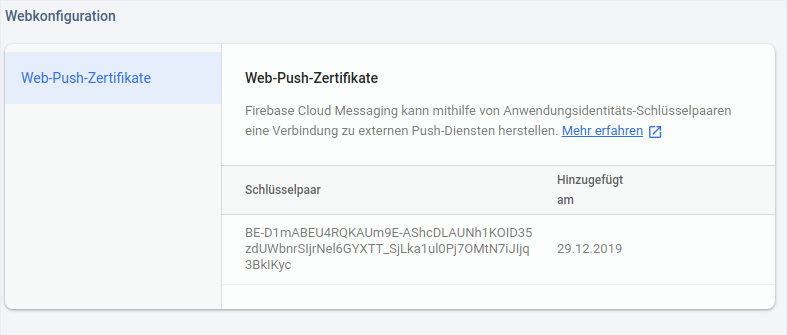
\includegraphics[width=\pictureWidth cm + 2 cm]{Bilder/Kapitel_4/firebase_webkonfiguration.png}
\caption{Firebase Webkonfiguration\label{fig:fcmwebconfig}}
\end{figure}

Für die Nutzung der \ac{FCM}-Funktionalitäten im Notification-Service der Hochschul-\ac{App} muss unter den Dienstkonten zuerst ein neuer privater Schlüssel erstellt werden. Dies sieht folgendermaßen aus:

\begin{figure}[H]
\centering
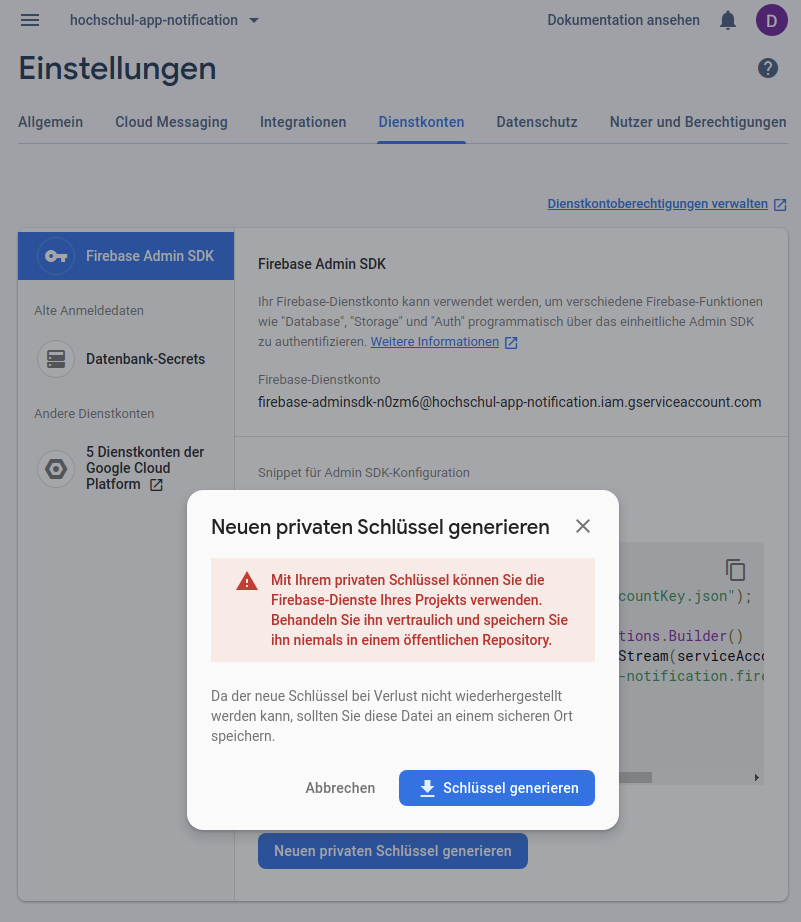
\includegraphics[width=\pictureWidth cm + 2 cm]{Bilder/Kapitel_4/fcm_privatekey.png}
\caption{Firebase Admin SDK Authentifizierung\label{fig:fcmprivatkey}}
\end{figure}

Nach diesem Schritt wird vom Firebase-Service ein \ac{JSON} generiert, welches alle relevanten Firebase-Service-Account Informationen wie Projekt-ID, Private-Key, Client-ID, Authentifikations-\ac{URL}, Tokens und die \acp{URL}  der Zertifikate enthält. Das komplette \ac{JSON}-File ist folgendermaßen aufgebaut:

\newpage
\begin{lstlisting}[caption={Firebase Service Account JSON}]
{
   "type": "service_account",
   "project_id": "hochschul-app",
   "private_key_id": "5ECUR3",
   "private_key": "-BEGIN PRIVATE KEY--END PRIVATE KEY-",
   "client_email": "firebase-adminsdk@hochschul-app.com",
   "client_id": "12345678",
   "auth_uri": "https://accounts.google.com/o/oauth2/auth",
   "token_uri": "https://oauth2.googleapis.com/token",
   "auth_provider_x509_cert_url": "https://www.google.com/certs",
   "client_x509_cert_url": "https://www.google.com/hochschul-app.com"
}
\end{lstlisting}

Dieses File muss dann im Notification-Service eingebunden werden. Dafür wird im \textit{application.properties}-File der Pfad des abgelegten \ac{JSON} definiert. Es wird dabei folgende Zeile angefügt: 

\begin{lstlisting}[caption={Firebase Service Account application.properties Datei}]
fcm.firebase-config-file=${PFAD}/firebase-adminsdk.json
}\end{lstlisting}

Im Package \textsc{config} des Source Codes des Notification-Service wird eine Klasse erstellt, die mit der Annotation \textsc{@ConfigurationProperties} markiert wurde und die Inhalte der \ac{FCM}-Properties in eine Variable schreibt.

\begin{lstlisting}[caption={Firebase Service Account Variable}]
@Setter
@Getter
@ConfigurationProperties(prefix = "fcm")
public class FcmProperties {

    private String firebaseConfigFile;

}
\end{lstlisting}

Zudem wird ein Bean der Konfigurationsklasse definiert und in den Notification Service eingebunden.

\newpage
\begin{lstlisting}[caption={Firebase Service Account Bean}]
@Configuration
@EnableConfigurationProperties(FcmProperties.class)
public class FcmPropertiesConfig {

    @Bean
    public FcmProperties fcmConfig () {
        return new FcmProperties();
    }

}
\end{lstlisting}

Mithilfe des Beans kann die Verbindung zur \ac{FCM}-Cloud dann folgendermaßen aufgebaut werden:

\begin{lstlisting}[caption={Firebase Service Account Bean}]
Path path = Paths.get(fcmPropertiesConfig.fcmConfig()
    .getFirebaseConfigFile());
InputStream inputStream = Files.newInputStream(path);
FirebaseOptions options = new FirebaseOptions
    .Builder()
    .setCredentials(
        GoogleCredentials
            .fromStream(inputStream)
    ).build();
\end{lstlisting}

Nach dem Verbindungsaufbau können im Notification Service Clients registriert sowie informiert werden. \ac{FCM} bietet zusätzlich die Möglichkeit der Erstellung von \textit{Topics}. Diese sind organisatorische Einheiten, in die Benachrichtigungen eingeteilt werden können. Somit muss sich ein Client nicht für alle Benachrichtigungen registrieren, sondern kann diese nach der Relevanz für seinen Anwendungsfall filtern.

\newpage
\begin{lstlisting}[caption={Firebase Service Account Bean}]
//build message with topic
Message message = Message.builder()
   .putAllData(messageTO.getData())
   .setTopic(topic)
   .setWebpushConfig(WebpushConfig.builder().putHeader("ttl", "300")
       .setNotification(new WebpushNotification(messageTO.getTitle(), messageTO.getBody(), icon))
       .build())
   .build();

//subscribe to topic
TopicManagementResponse response = FirebaseMessaging.getInstance()
    .subscribeToTopicAsync(
        Collections.singletonList(registrationToken), 
        topic
    ).get();

//unsubscibe from topic
TopicManagementResponse response = FirebaseMessaging.getInstance()
    .unsubscribeFromTopicAsync(
        Collections.singletonList(registrationToken), 
        topic
    ).get();

//send message
FirebaseMessaging.getInstance().sendAsync(message).get();

\end{lstlisting}
\chapter{Entwicklungsumgebungen}
\label{sec:environments}

Wie in allen größeren Software Projekten ist es in der Regel üblich, zwei verschiedene Einrichtungen für die Anwendung in den verschiedenen Phasen ihrer Existenz zu verwenden. Dabei unterscheidet man in der Regel von der Entwicklungsumgebung in der Entwicklungsphase und der Umgebung in der Produktionsphase. Passend zu ihren Einsatzzwecken werden diese Umgebungen jeweils \textit{dev} und \textit{prod} genannt. Auch der Prototyp der Hochschul Anwendung verfügt über diese beiden Konfigurationen. Warum diese benötigt werden und wie sie im Detail aufgebaut sind, beziehungsweise was sie genau unterscheidet, wird im folgenden genauer betrachtet.

\section{Dev-Environment}

Die Umgebung, die den Entwicklern beim Arbeiten an der Anwendung zur Verfügung steht, zeichnet sich vor allem in drei Punkten aus: der Datenbankanbindung, der Kommunikation innerhalb der Services und des Starts der Anwendung. Diese drei Punkte wurden einerseits so angepasst, dass der Entwickler einfacher Änderungen vornehmen kann, aber auch so, dass den Anbindungen der nur im Produktionsmodus der Anwendung benötigten Ressourcen nicht durch versehentliche Fehler geschädigt werden. Die genauen Eigenschaften werden nun kurz erläutert.

\subsubsection{Datenbankanbindung}

Die Datenanbindung der Hochschul-\ac{App} benötigt Zugriffe auf verschiedene Datenbanken. Einerseits werden Datenbanken angelegt, die für den internen Gebrauch der Services benötigt werden. Dazu gehören die Datenbanken für die Mensa Daten, Stundenplaninformationen aber auch die User-spezifischen Daten. Andererseits werden ebenfalls die Daten des \textit{LxLehre}-Servers der Hochschule benötigt. Dieser enthält die aktuellen Stundenplan-Daten und ist aktuell noch als Proxy-Datenbank zwischen die Services und die Datenbank der Hochschule Hof geschaltet. Beide Arten von Datenbanken benötigen eine gültige \textit{MySQL} Installation, auf der sie laufen können. Würde dies auch im Entwicklungszeitraum benötigt werden, würden sich zwei Alternativen anbieten. Entweder, jeder Entwickler installiert MySQL auf seinem \ac{PC} und richtet die Datenbanken als perfekte Abbilder zu ihren Originalen auf den Hochschul-Servern ein oder es werden die echten Datenbanken eingebunden. Die erste Lösung bietet keine flexiblen Änderungen an der Datenbank und erfordert, das die Datenbanken auf jedem System einzeln installiert werden. Die zweite Möglichkeit sollte gar nicht erst in Betracht gezogen werden, da jeder Fehler der Entwickler sich sofort auf die originalen Daten auswirkt.\\
\linebreak
Deshalb wurde in der  \textit{dev}-Entwicklungsumgebung die Datenbank \textit{H2} eingebunden. Diese Datenbank ist eine reine In-Memory Datenbank, welche ihre Konfiguration aus einer statischen Datei mit Testdaten sammelt. Diese sind eine Spiegelung der originalen Daten. Beim Start der Anwendung wird hierbei jedes Mal die \textit{H2} Datenbank neu initialisiert, wobei Fehler aus alten Starts der Anwendungen nicht beachtet werden. Diese \textit{H2} Datenbank enthält alle Tabellen, die vom System benötigt werden, weshalb die Einbindung mehrerer Datenquellen nicht mehr nötig ist. Des weiteren muss der Entwickler keine zusätzliche Software auf seinem System installieren, da die \textit{H2} Datenbank über eine Java-Bibliothek läuft. Wie man es aus anderen \acp{DBMS} kennt, gibt es für die \textit{H2} Datenbank eine grafische Benutzeroberfläche, über welche die Daten eingesehen und mit Standard-\ac{SQL} abgeändert werden können. Diese ist mit jedem Browser unter folgender \ac{URL} erreichbar:

\begin{lstlisting}[caption={H2-Console}]
https://localhost:[port-des-services]/h2-console
\end{lstlisting}

Über diese \ac{URL} gelangt man - insofern der Service im \textit{dev}-Modus gestartet wurde - auf folgende Oberfläche:

\begin{figure}[H]
\centering
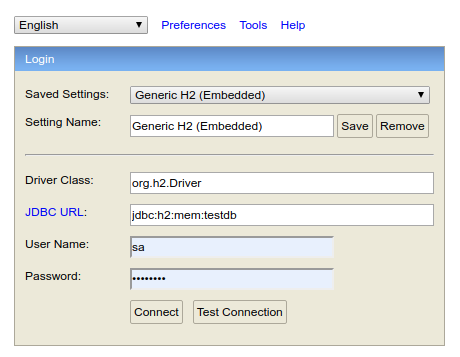
\includegraphics[width=\pictureWidth cm]{Bilder/Kapitel_5/h2_login.png}
\caption{Login der \textit{H2}-Console\label{fig:h2_login}}
\end{figure}

Der Login erfolgt über den Nutzernamen und das Passwort, die in der \textit{application-dev.properties}-Datei hinterlegt wurden. Nach dem Login wird dann ein Textfeld angezeigt, in dem \ac{SQL}-Satements auf alle in der linken Seite der Oberfläche angezeigten Tabellen ausgeführt werden können.

\subsubsection{Microservice Kommunikation}

Anders als im \textit{prod}-Modus einer Anwendung, können alle Teile der Anwendungen, darunter auch die Microservices, individuell gestartet werden. Dabei sind keine weiteren Services nötig, alle Abhängigkeiten werden in der Test Umgebung simuliert. Somit müssen bei Abhängigkeiten zwischen den Microservices keine anderen Services gestartet werden. Da dies in einer Microservice Architektur im allgemeinen nicht vorgesehen ist, sind hierbei vor allem das \ac{API}-Gateway und der \textit{Eureka}-Server zu betrachten. In der Entwicklungsumgebung muss zuerst der \textit{Eureka}-Server gestartet werden, worauf das \ac{API}-Gateway sich dann bei seinem Start beim \textit{Eureka}-Server registrieren kann. Danach können alle anderen Services gestartet werden. Im \textit{dev}-Modus ist das nicht der Fall, hier sind Gateway- und Service-Discovery-Funktionen deaktiviert. Dies geschieht über Konfigurationen in der \textit{application-dev.properties}-Datei, die benötigten Eigenschaften sehen wie folgt aus:

\newpage
\begin{lstlisting}[caption={Discovery und Gateway Deaktivierung}]
eureka.client.enabled=false
eureka.client.register-with-eureka=false
\end{lstlisting}


\subsubsection{Start der Anwendung}

Der wohl gravierendste Unterschied zwischen der produktiven und der Entwicklungsumgebung liegt im Start der Anwendung. Möchte man einen Teil der Anwendung starten, um ihn in der \textit{dev}-Umgebung zu testen, so benötigt man dazu, wie bereits erwähnt, keine Instanzen des \textit{Eureka}-Servers oder des \ac{API}-Gateways. Man stößt lediglich die Kompilierung und den Build-Prozess des Services an und startet die danach generierte \textit{*.jar}-Anwendung mit dem Konsolenbefehl \textsc{java -jar [dateiname].jar}.\\
\linebreak
Um dies Prozesse jedoch nicht manuell anstoßen zu müssen sind die im Kapitel \ref{sec:entwicklungsumgebung} beschriebenen Tools hilfreich. Durch die \ac{IDE} kann der Programmcode automatisch kompiliert, gebuilded und gestartet werden. Das alles sogar im sogenannten \textit{Debug}-Modus der \ac{IDE}, welcher es ermöglicht, Breakpoints im Code zu setzen, bei deren Durchlaufen das Programm gestoppt wird, um die Variablen während der Laufzeit auslesen zu können. In der in dieser Praxisarbeit empfohlenen \ac{IDE} sind die Buttons zum Start und zum Debuggen der Anwendung rechts oben in der Oberfläche zu finden. Diese sehen wie folgt aus:

\begin{figure}[H]
\centering

\includegraphics[width=\pictureWidth cm]{Bilder/Kapitel_5/ide_start_prog.png}
\caption{Start und Debuggen der Anwendung in der \ac{IDE}\label{fig:ide_start_prog}}
\end{figure}

Der Linke der markierten Buttons ist zum Start der Anwendung im normalen Modus zuständig. Dabei ist kein Debugging möglich, es werden beim Ausführen der Anwendung jedoch auch weniger Ressourcen des Systems benötigt. Der Rechte der beiden Buttons ist der Debug Button. Durch diesen können im Code Breakpoints gesetzt werden, die die Anwendung auch stoppen. Dieser Modus benötigt jedoch mehr Systemressourcen. Anzumerken ist ebenfalls, das beide Modi das erwähnte Hot-Deployment aus Kapitel \ref{sec:hot_deploy} unterstützen. 

\subsubsection*{Einrichtung des \textit{dev}-Modus}

Die \ac{IDE} \textit{IntelliJ IDEA} erleichtert es ungemein, eine Einstellung für die Entwicklung im \textit{dev}-Modus zu erstellen. Hierfür öffnet man lediglich das im rechten oberen Bildrand befindliche Dropdown und wählt \textit{Edit Configurations...} aus. Danach erscheint folgendes Menü:

\begin{figure}[H]
\centering
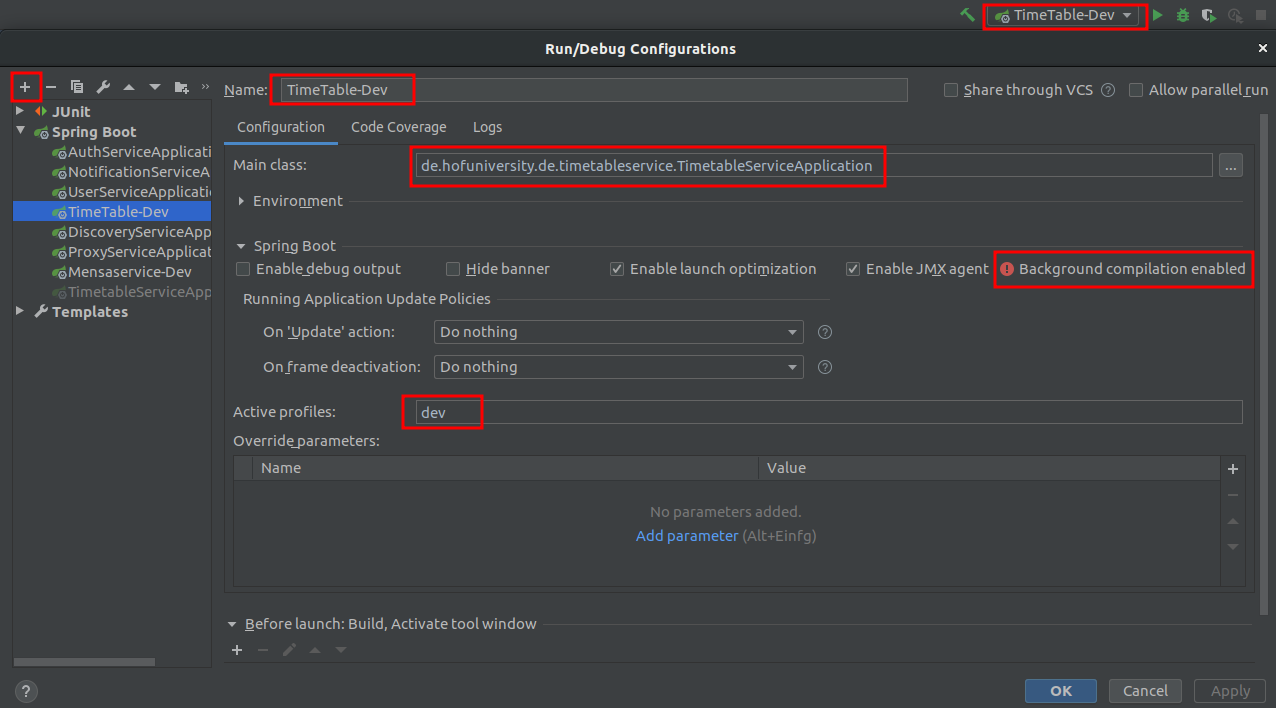
\includegraphics[width=\pictureWidth cm + 2 cm]{Bilder/Kapitel_5/ide_dev_config.png}
\caption{Einstellen der Test-Umgebung in der \ac{IDE}\label{fig:ide_dev_config}}
\end{figure}

Die in der Abbildung \ref{fig:ide_dev_config} markierten Felder werden nun von oben nach unten und von links nach rechts erläutert:

\begin{itemize}
\item Auswählen von \textit{Edit Configurations...} im Dropdown
\item Erstellen einer neuen \textit{Spring} Konfiguration
\item Vergeben eines Namens für die Konfiguration
\item \textit{! Background compilation enabled} sollte angezeigt werden, da dies in der Einrichtung zum Hot-Deployment in Kapitel \ref{sec:hot_deploy} eingerichtet wurde. 
\item Zuordnung zum \textit{Active Profile} \textsc{dev} (Der Name ist hier frei wählbar, wird aber später gebraucht)
\end{itemize}

Zusätzlich muss nun in den Ressourcen des Microservices eine neue Properties-Datei erstellt werden, die nach folgendem Schema benannt werden muss:\\
\textit{application-}\textsc{dev}\textit{.properties}\\
\textsc{dev} ist hierbei der Name des \textit{Active Profile}, welches vorher konfiguriert wurde. In diesem Properties-File können nun alle Konfigurationen für die Testumgebung hinterlegt werden, die \textit{dev}-Konfiguration, die in der \ac{IDE} vorgenommen wurde, lädt diese dank der Namensgebung automatisch. Das Properties-File hat den selben Aufbau und Zweck wie das in Kapitel \ref{sec:resources} erklärte File.

\section{Prod-Environment}

Das starten der Services auf der produktiven Umgebung bedarf einer festgelegten Vorgehensweise. Hierbei ist die Reihenfolge der Schritte, die im folgenden kurz aufgelistet werden, kritisch.

\begin{enumerate}
\item Start des \textit{Eureka}-Servers
\item Start des \ac{API}-Gateways
\item Start der anderen Services
\end{enumerate}

Das Starten der Services erfolgt nach dem Erstellen der einzelnen \textit{*.jar}-Dateien für jeden Service. Diese werden dann mit folgendem Befehl gestartet:

\begin{lstlisting}[caption={Starten eines \textit{jar}-Files}]
~: java -jar [dateiname].jar
\end{lstlisting}

Da die Reihenfolge dieses Vorgangs kritisch ist und beliebig viele Services gestartet werden können, bietet sich es an, diesen Vorgang per Skript zu automatisieren. In diesem Zug kann man auf die Ausgabe der Programme in eine Log-Datei weiterleiten und die Anwendung im Allgemeinen beobachten. Ein passendes Skript auf einer UNIX-basierten Umgebung könnte wie folgt aussehen:

\newpage
\begin{lstlisting}[caption={Skript zum Verwalten der Microservices}]
#!/bin/sh
#repeat each step per *.jar files 
#needed in correct order

#Start API packaged in microservice.jar
start(){
    #Create .log directory
    mkdir .log > /dev/null 2>&1
    echo "Starting API on port 8080"
    #Start timetableAPI.jar, Redirect Error and Output to logfile
    java -jar ~/microservice.jar >> ~/.log/microservice.log 2>&1 &
    echo "Started API"
}

#Stop API Process running on tcp port 8080
stop(){
    echo "Stopping API on port 8080"
    #fuser finds processfile, -k kills process
    fuser -k 8080/tcp
    echo "Stopped API"
}

#Checking status of API running on tcp port 8080
status(){
    #if fuser finds process for port 8080
    if fuser 8080/tcp then
        echo "API running on port 8080"
    else
        echo "API not running"
    fi
}

restart(){
    echo "Stopping API to reload"
    stop
    start
    echo "Successfully restarted API"
}

#Switch params to call functions
case $1 in
start)
    start
;;
stop)
    stop
;;
status)
    status
;;
restart|reload)
    restart
;;
*)
    echo "Usage: $0 (start|stop|status|restart|reload)"
    exit 1
esac

#End script
exit 0
\end{lstlisting}
\chapter{Microservice Dokumentation}
\label{sec:microserviceswagger}

Wie bereits an mehreren Stellen in dieser Arbeit erwähnt wurde, wird zur Dokumentation der Microservices und deren Endpunkte das Framework \textit{Spring-Fox} verwendet. Dieses baut auf dem weit verbreiteten Standard \textit{Swagger} auf. \textit{Swagger} ermöglicht es, Endpunkte standardisiert in Form von \ac{YAML}-Dokumenten zu dokumentieren, deren Nutzung zu erklären und die möglichen Datenabfragen aufzulisten. Im folgenden Kapitel soll nun erläutert werden, wie das \textit{Spring-Fox}-Framework eingebunden wurde, wie die Endpunkte damit dokumentiert wurden und wie ein Nutzen aus diesem Framework gezogen werden kann.

\section{Konfiguration im Microservice}

Wie bereits im Kapitel \ref{sec:annotations} beschrieben wurde, werden für die Nutzung von \textit{Spring-Fox} im Prototypen der Hochschul-\ac{App} zwei Abhängigkeiten benötigt. Diese werden im \textsc{pom.xml} der einzelnen Services folgendermaßen eingebunden:

\begin{lstlisting}[caption={Einbinden der \textit{Spring-Fox}-Abhängigkeiten}]
<dependency>
    <groupId>io.springfox</groupId>
    <artifactId>springfox-swagger2</artifactId>
    <version>2.9.2</version>
</dependency>
<dependency>
    <groupId>io.springfox</groupId>
    <artifactId>springfox-swagger-ui</artifactId>
    <version>2.9.2</version>
</dependency>
\end{lstlisting}

Zusätzlich muss nun noch im \textit{src}-Package des Quellcodes ein Konfigurations-Bean erstellt werden, das mit der Annotation \textsc{@EnableSwagger2} und \textsc{@Configuration} markiert werden muss. Diese Bean-Klasse kann wie folgt aussehen:

\newpage
\begin{lstlisting}[caption={Bean zur Swagger Konfiguration im Mensa-Service}]
@Configuration
@EnableSwagger2
public class SwaggerConfig {

    @Bean
    public Docket api() {
        return new Docket(DocumentationType.SWAGGER_2)
            .useDefaultResponseMessages(false)
            .directModelSubstitute(LocalDate.class, String.class)
            .select()
            .apis(RequestHandlerSelectors
              .basePackage("de.hofuniversity.mensaservice"))
            .paths(regex("/menu.*"))
            .build()
            .apiInfo(metaInfo())
            .tags(new Tag("Mensa Controller", "The resource manages the creation, reading and deletion of all dishes"),
                  new Tag("Dish Controller", "The resource manages the update, reading and deletion of specific dish"),
                  new Tag("Filter Controller", "The resource manages the creating, update, reading and deletion of possible filter query parameters"),
                  new Tag("Menu Date Controller", "The resource manages the reading of all dishes depending on dates"),
                  new Tag("Menu Week Controller", "The resource manages the reading of all dishes depending on calender week and also day of the week"));
    }

    private ApiInfo metaInfo() {
        return new ApiInfoBuilder()
            .title("Mensa-Service API")
            .description("The service provides the client with all information about dishes and also allows them to filter, sort and to personalize")
            .version("1.0.0")
            .contact(new Contact("Dennis Brysiuk", "", "dennis.brysiuk@hof-university.de"))
            .termsOfServiceUrl(
              "https://www.hof-university.de/impressum.html"
            ).build();
    }
}
\end{lstlisting}

Es werden kurz die Methoden und deren Inhalte erläutert:

\begin{itemize}
\item \textbf{new Docket(...)}\\
Erstellt neues Docket, das \ac{API} Informationen generiert
\item \textbf{apis(...)}\\
Fügt dem Docket eine Liste von \ac{API}-Dokumentationen hinzu
\item \textbf{paths(...)}\\
Zeigt dem Docket, für welche Endpunkte Doku generiert werden muss
\item \textbf{tags(...)}\\
Teilt die Endpunkte in Kategorien ein, die im Controller definiert werden
\item \textbf{new ApiInfoBuilder()}\\
Erstellt allgemeine Infos zur \ac{API}
\item \textbf{title(...)}\\
Gibt der \ac{API} einen Titel
\item \textbf{description(...)}\\
Beschreibt die \ac{API}
\item \textbf{version(...)}\\
Gibt die Versionsnummer der \ac{API} an
\item \textbf{contact(...)}\\
Fügt der Dokumentation eine Referenzperson an
\item \textbf{termsOfServiceUrl(...)}\\
Erstellt einen Link zum Impressum
\end{itemize}

\section{Controller Beschreibung}

In der Konfigurations-Klasse wurden bereits allgemeine Informationen zur gesamten \ac{API} hinterlegt, darunter auch die Information, welche Endpunkte gescant und dokumentiert werden sollen. Dennoch müssen nun genauere Informationen zu den Endpunkten in den Controller Klassen einer \ac{API} annotiert werden. Das sieht am auf Klassenebene folgendermaßen aus:

\begin{lstlisting}[caption={Swagger Konfiguration auf Controller Ebene am Beispiel des Timetable Controllers}]
@RestController
@RequestMapping("/lectures")
@ApiResponses(value = {
        @ApiResponse(code = 400, message = "Incorrect request from the client", response = HttpReturnErrorPattern.class),
        @ApiResponse(code = 401, message = "Request for the resource requires authorization", response = HttpReturnErrorPattern.class),
        @ApiResponse(code = 403, message = "You do not have sufficient authorization for this action", response = HttpReturnErrorPattern.class),
        @ApiResponse(code = 404, message = "The requested resource was not found by the server", response = HttpReturnErrorPattern.class),
        @ApiResponse(code = 500, message = "The request cannot be processed dues to an unexpected error on the server", response = HttpReturnErrorPattern.class)
})
@Api(tags = {"Timetable Information"})
public class TimetableController {
...
\end{lstlisting}

Folgende Annotationen können auf Controller Ebene nun die Endpunkte genauer beschrieben:

\begin{itemize}
\item \textbf{@ApiResponses(value=[Array of ApiResponse])}\\
Erstellt eine Sammlung von \ac{HTTP}-Responses, die für alle in der Klasse definierten Endpunkt-Methoden gelten
\item \textbf{@ApiResponse(...)}\\
Erstellt genaue Informationen zu einer \ac{HTTP}-Response
\item \textbf{@Api(tags=[tags])}\\
Ordnet die Controller Klasse zu einem in der Konfiguration definiertem Tag hinzu
\end{itemize}

\section{Dokumentation der Funktionen}

Die auf Controller Ebene definierten Dokumentationen werden auf alle Methoden der Controller Klasse angewendet. Dennoch kann es sein, dass eine der Methoden für eine bereits auf Controller Ebene definierte Antwort eine andere Definition dokumentieren will oder eine \ac{HTTP}-Response produziert, die alle anderen Methoden so nicht produzieren können. Diese Responses können nun auf Methoden Ebene überschrieben oder neu definiert werden. Des weiteren können hier die Dokumentationen zu den einzelnen Parametern festgelegt werden. Eine annotierte Methode könnte nun folgendermaßen aussehen:

\begin{lstlisting}[caption={Swagger Konfiguration auf Methoden Ebene am Beispiel des Semester Controllers}]
@ApiOperation(value="Get number of semesters for given program", response = SemesterListTO.class)
    @ApiResponses( value={
            @ApiResponse(code=OK, message = "Successfully retrieved semesters for given program", response = SemesterListTO.class),
    })
    @ResponseStatus(value = HttpStatus.OK)
    @GetMapping
    public SemesterListTO getSemesters(
            @ApiParam(name = "Faculty Id", value = "Unique identifier for a faculty", required = true, example = "INF")
            @PathVariable("faculty") String facultyId,
            @ApiParam(name = "Program Id", value = "Unique identifier for a program", required = true, example = "MB")
            @PathVariable("program") String programId){
\end{lstlisting}

\begin{itemize}
\item \textbf{@ApiOperation(...)}\\
Liefert genaue Informationen zur Methode und der zu erwartenden Antwort\\
\linebreak
\item \textbf{@ApiResponses(value=[Array of ApiResponse])}\\
Erstellt eine Sammlung von \ac{HTTP}-Responses, die für die annotierte Methode gelten
\item \textbf{@ApiResponse(...)}\\
Erstellt genaue Informationen zu einer \ac{HTTP}-Response
\item \textbf{@ApiParam(...)}\\
Beschreibt den zu übergebenen Parameter genau
\end{itemize}

\section{Export der Dokumentation}

Die große Stärke des \textit{Swagger}-Standards ist das einfache lesen der erstellten \ac{YAML}-Dateien. Jedoch wurde \textit{Swagger} dahingehend erweitert, dass es nun auch Dokumentationen in anderen Formaten unterstützt, die von Maschinen leichter prozessiert werden können. Unter anderem werden nun auch Dokumentationen in \ac{JSON} unterstützt. Eine genau solche Dokumentation kann für jeden Service automatisch generiert und exportiert werden, indem man bei laufendem Service folgende \ac{URL} aufruft:

\begin{lstlisting}[caption={Swagger Export URL}]
http://localhost:[port-of-service]/[version]/api-docs
\end{lstlisting}

\section{Nutzen der grafischen Oberfläche}

Aus der oben genannten Dokumentation kann das \textit{Spring-Fox} Framework ebenfalls eine grafische Oberfläche generieren, mit welcher die Dokumentation besser gelesen und die Endpunkte sogar getestet werden können. Diese grafische Oberfläche kann über folgende \ac{URL} aufgerufen werden:

\begin{lstlisting}[caption={Swagger Export URL}]
http://localhost:[port-of-service]/swagger-ui.html
\end{lstlisting}

Beim Aufrufen dieser \ac{URL} wird dem Nutzer folgende Oberfläche angezeigt. Für dieses Beispiel wurde der Timetable-Service genutzt.

\begin{figure}[H]
\centering
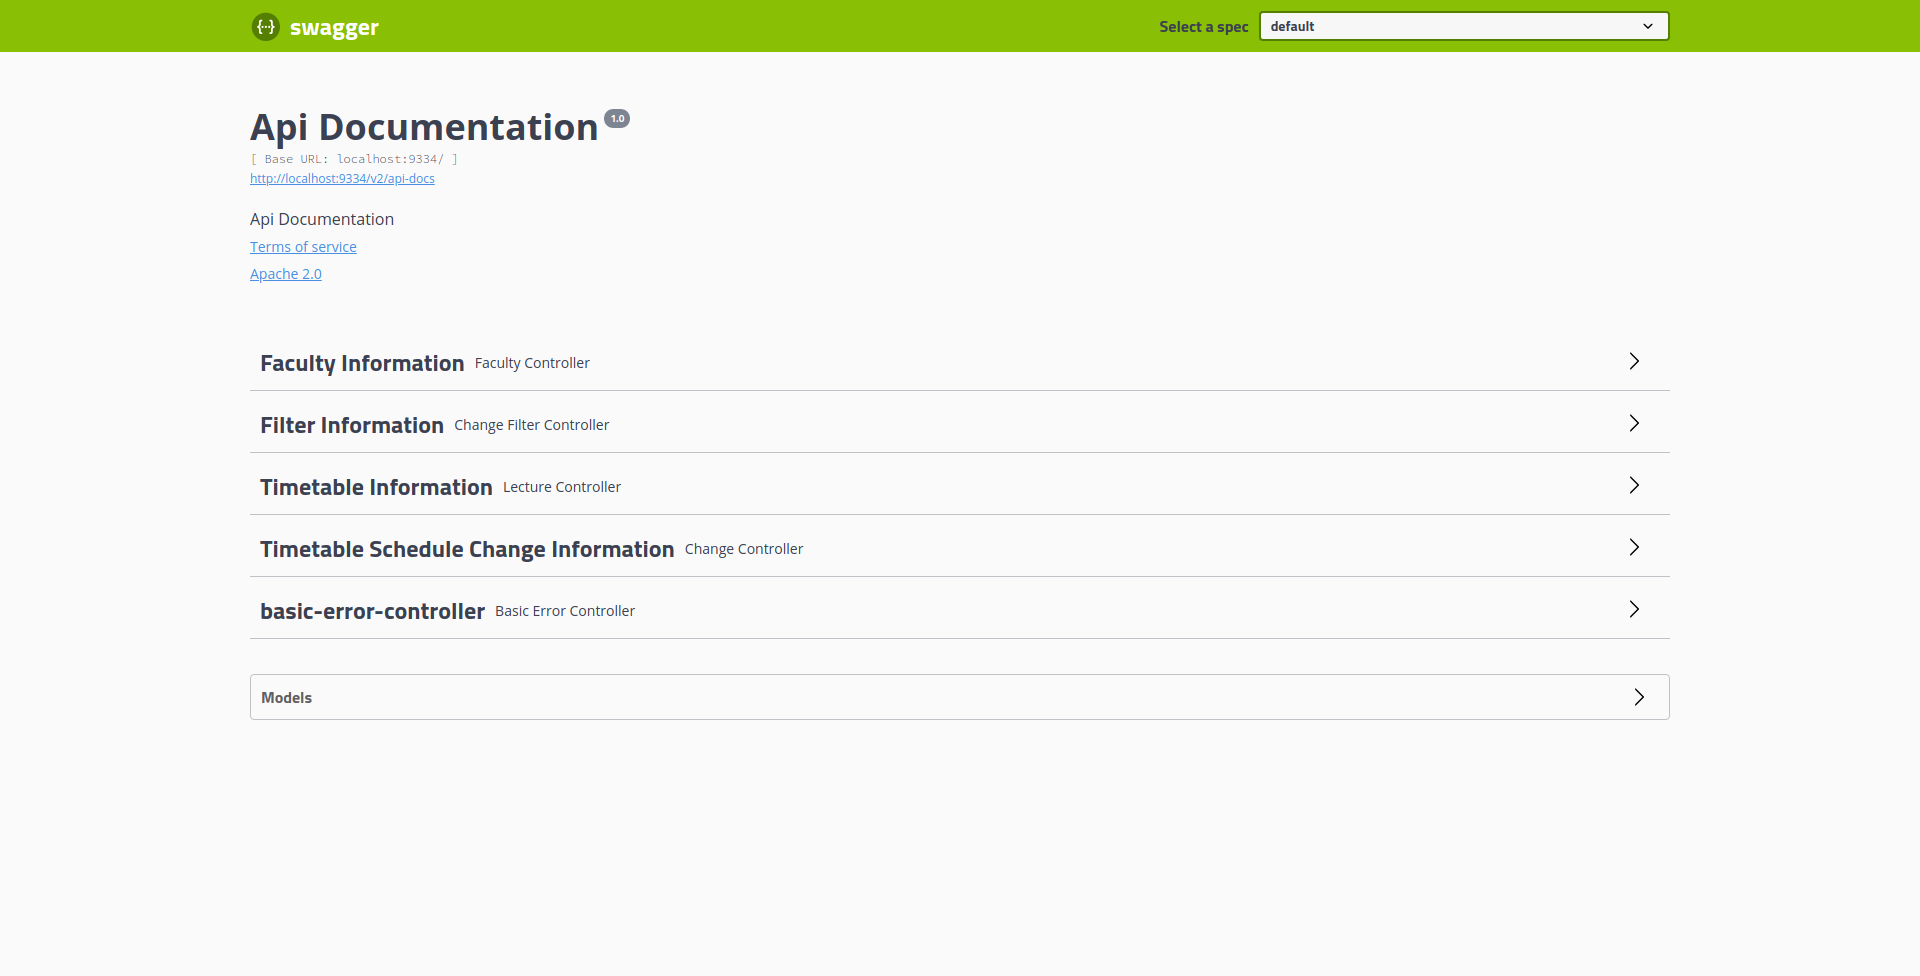
\includegraphics[width=14 cm]{Bilder/Kapitel_6/swagger_ui.png}
\caption{Swagger UI am Beispiel des Timetable-Service\label{fig:swagger_ui}}
\end{figure}

Klappt man nun eines der Controller Felder auf, so werden alle in diesem Controller verfügbaren Methoden und Endpunkte mitsamt ihrer Beschreibungen und \acp{URL} aufgelistet.

\begin{figure}[H]
\centering
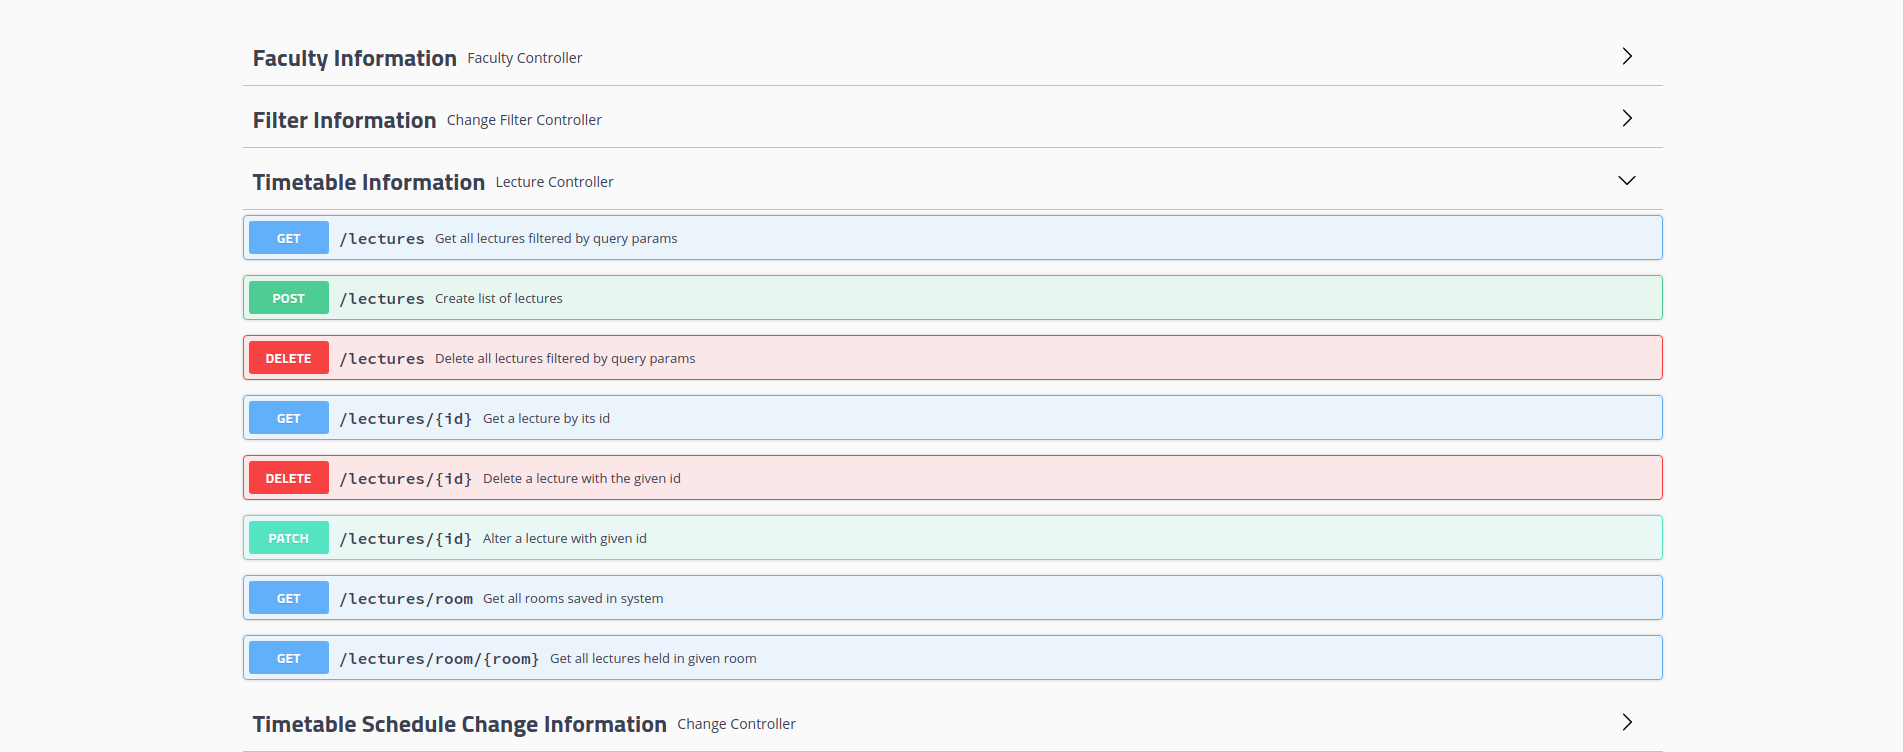
\includegraphics[width=14 cm]{Bilder/Kapitel_6/swagger_ui_methoden.png}
\caption{Swagger UI Timetable Methoden\label{fig:swagger_ui_methods}}
\end{figure}

Beim Auswählen einer der Methoden werden alle Details zu dieser einzelnen Methode angezeigt. Dazu gehören unter anderem auch alle möglichen Rückgabewerte, die Parameter, die von der Ressource akzeptiert werden und die zulässigen Werte, die in diesen Parametern übergeben werden können.

\begin{figure}[H]
\centering
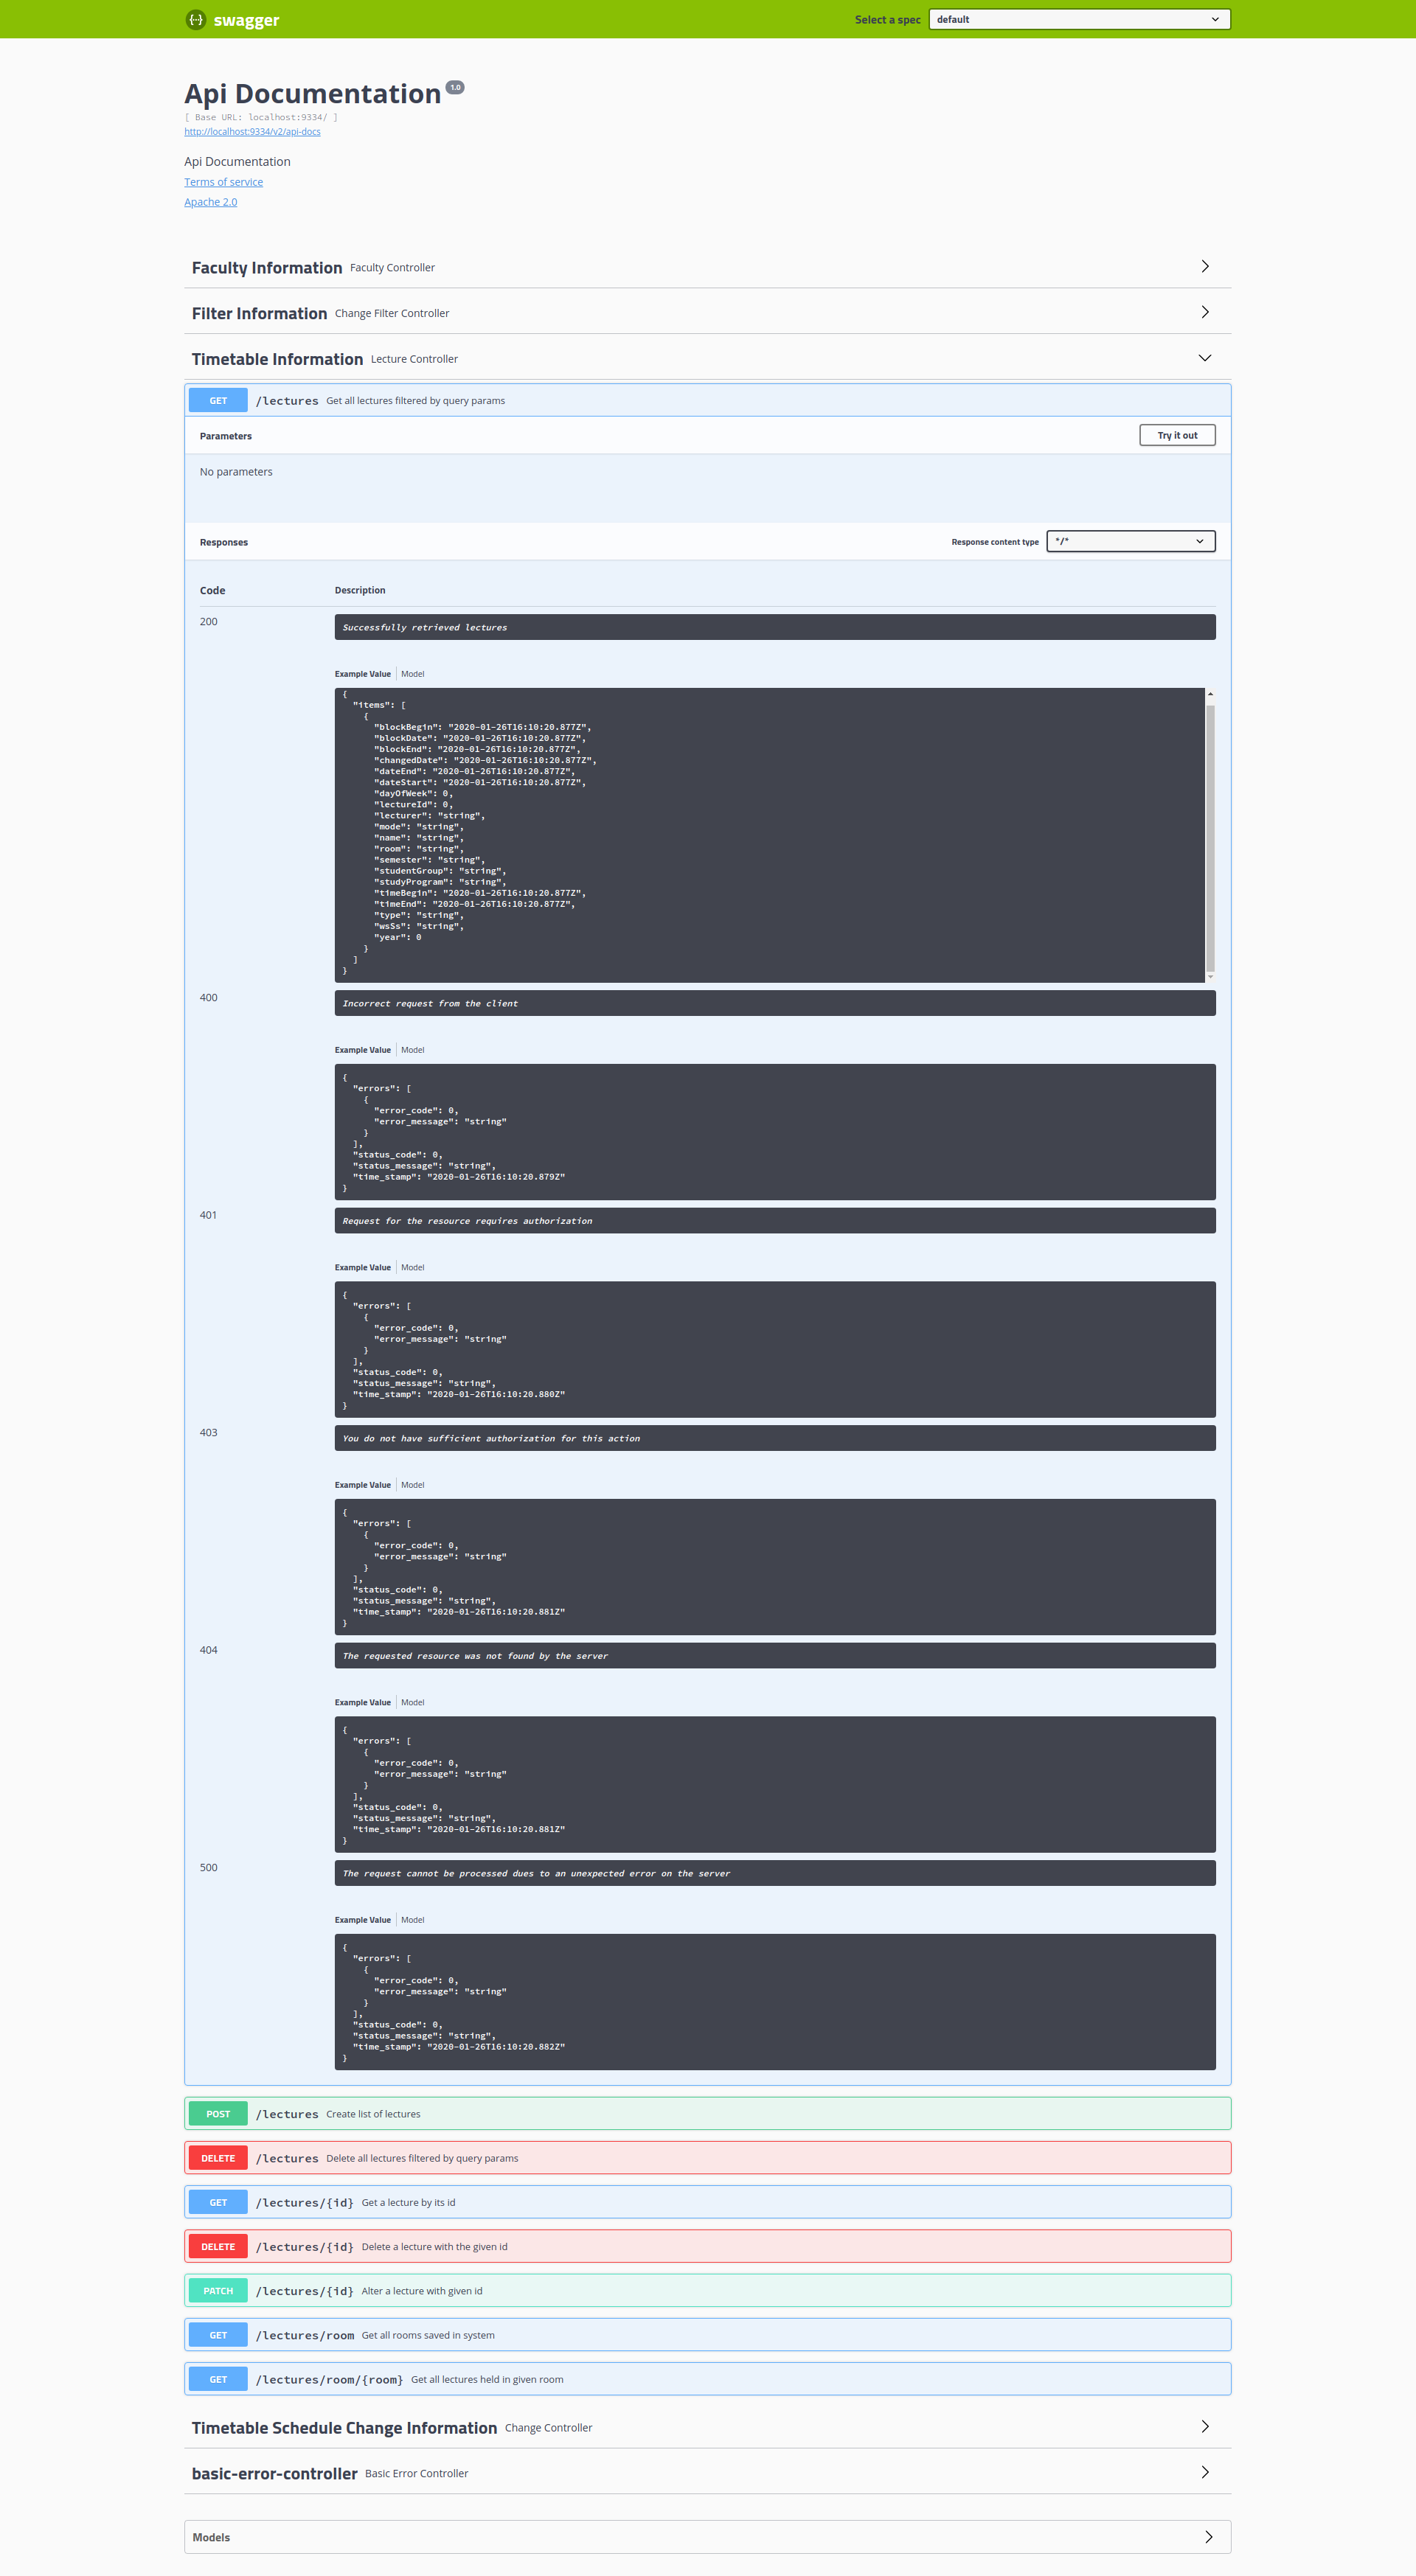
\includegraphics[width=12 cm]{Bilder/Kapitel_6/swagger_ui_method_detail.png}
\caption{Swagger UI Timetable Methoden Details\label{fig:swagger_ui_method_detail}}
\end{figure}

Wählt man nun im oberen rechten Eck der ausgewählten Ressource den Button \textit{Try it out!}, so wird dem Nutzer eine Ansicht präsentiert, die ihm die Möglichkeit gibt, alle Übergabeparameter einzugeben, die erlaubten Header für die \ac{HTTP} Anfrage zu konfigurieren und die Anfrage abzusenden. Die Anfrage wird dann an den Server weitergeleitet und ausgeführt. Hierbei ist anzumerken, dass die Anfragen unumkehrbar ausgeführt werden und nicht nur simuliert sind. Darauf präsentiert die \textit{Swagger-UI} dem Nutzer folgende Darstellung der Antwort des Servers:

\begin{figure}[H]
\centering
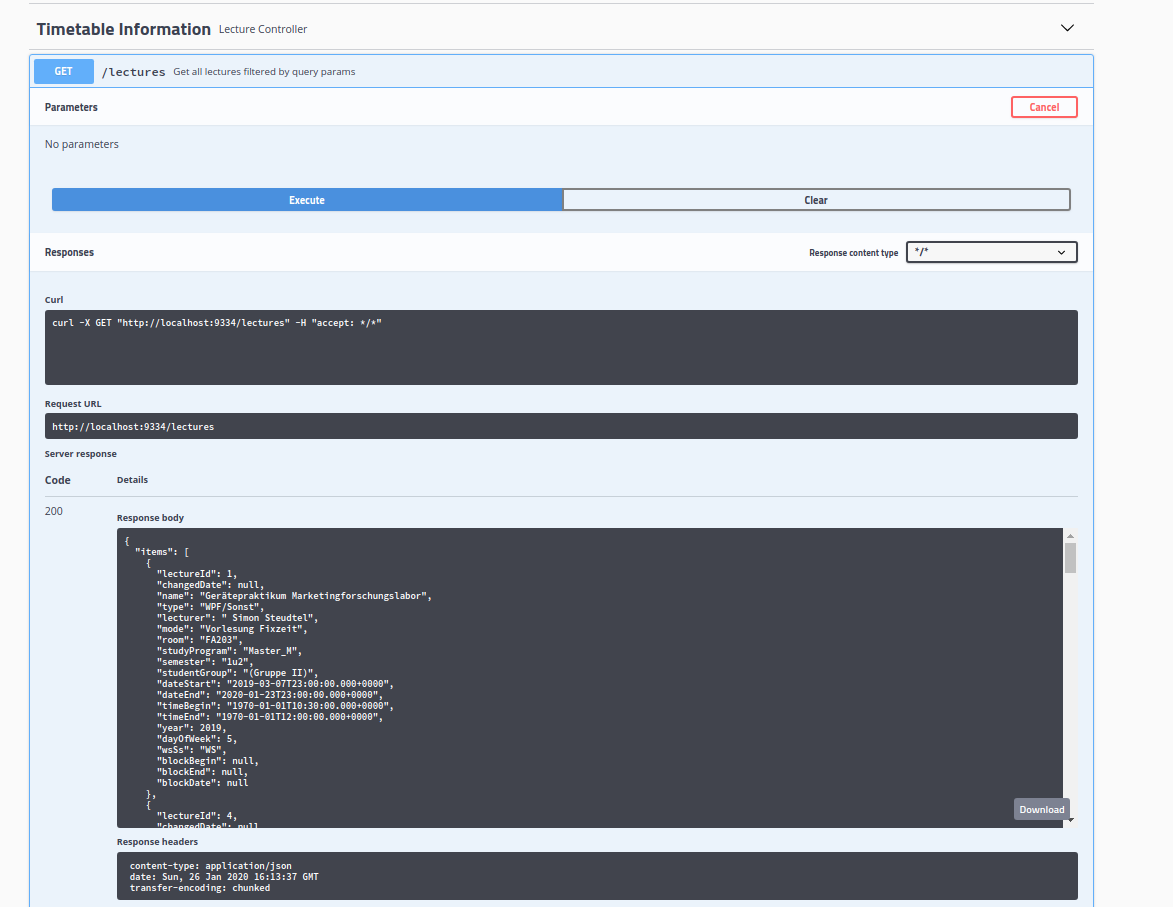
\includegraphics[width=14 cm]{Bilder/Kapitel_6/swagger_ui_try.png}
\caption{Testen einer Anfrage in der Swagger UI\label{fig:swagger_ui_try}}
\end{figure}
\chapter{Testing}
\label{sec:test}

Wie in jedem Software Projekt wurden auch im Falle des Prototypen der neuen Hochschul-\ac{App} Tests durchgeführt. Diese ermöglichen es, unvorhergesehene Fehler oder Sicherheitslücken im Vornherein zu einem gewissen Grat auszuschließen. Um Microservices in \textit{Spring} zu Testen reichen zwei Arten von Tests, Integrationstests und Unit-Tests. Integrationstests dienen dazu, verschiedene voneinander abhängige Komponenten eines komplexen Systems im Zusammenspiel zu testen. Wichtig ist hierbei, dass manche Komponenten integriert werden müssen, also werden fehlende Module simuliert und andere Komponenten werden gleichzeitig zusammengefügt und in das zu testende System integriert. In Unit-Tests hingegen werden lediglich die Einzelteile des Systems isoliert auf ihre korrekte Funktionalität geprüft.\\
\linebreak
Die Test-Frameworks für Integrationstests und Unit-Tests stellt \textit{Spring Boot} mit dem Framework \textit{sping-boot-starter-test} zu Verfügung. Dieses muss lediglich über eine Maven-Dependency in das Projekt eingefügt werden. Außerdem muss noch eine \textit{H2}-Datenbank als \textit{Maven}-Dependency eingefügt werden. Eine \textit{H2}-Datenbank ist eine In-Memory Datenbank. Diese wird für das Testen des Datenschicht benötigt und wurde bereits ausführlicher im Kapitel \ref{sec:environments} beleuchtet.\\
\linebreak
Da bei vielen Software Projekten die maximal mögliche Testabdeckung erreicht werden muss, werden dort in der Regel unzählige Stunden und Ressourcen in den Testvorgang investiert. Da dies den Rahmen dieser Arbeit deutlich sprengen würde werden nicht alle Schichten der Gesamtsoftware getestet. Um dennoch eine möglichst große Wahrscheinlichkeit zu erreichen, alle groben Fehler eliminiert zu haben, werden sowohl die Serviceschicht, die Controller-Schicht als auch die Util Klassen getestet.\\
\linebreak
Im folgenden werden nun nicht alle Testfälle angeführt, da dies oft redundante Fälle sind, die sich nur in Details unterscheiden. Stattdessen wird von jeder Art der Tests ein Fall exemplarisch erläutert und genauer betrachtet. Allgemein gilt für alle Testfälle, dass die Annotation \textsc{@RunWith(SpringRunner.class)} an die Testklasse angehängt werden muss, damit das \textit{Spring Boot} Framework eine Verbindung zu den Funktionen des Test-Framework \textit{JUnit} aufbauen kann.

\section{Controller Tests}

Klassische Unit-Tests können an Controller-Klassen nicht angewendet werden. Diese bilden einen Sonderfall, denn sie behandeln im Laufe der Anwendung Anfragen mit dem \ac{HTTP}-Protokoll, reichen diese an die Serviceschicht weiter und liefern lediglich eine Antwort an den aufrufenden Client. Hierbei ist es also notwendig, dass das \textit{Spring Boot} Framework die nötige \ac{HTTP}-Unterstützung bereitstellt. Hierbei geht es konkret um die Funktionen zur Serialisieren und Deserialisieren von Eingabeparametern, die durch die Annotations \textsc{@RequestBody},\textsc{@PathParam} und \textsc{@PathVariable} markiert sind und durch die Annotation \textsc{@Valid} validiert werden müssen\autocite[][]{controller_test}.\\
\linebreak
Des weiteren werden alle benötigten Abhängigkeiten oder Beans bei den Tests ignoriert, man kann sogar so weit gehen und die Autokonfiguration des Controllers durch die Annotation \textsc{@WebMvcTest(Controller.class)} verhindern, wenn dies gewünscht ist. So können alle benötigten Konfigurationen simuliert werden. Auch das Starten des Servers kann ausgespart werden, wenn die Test-Klasse mit \textsc{@MockMvc} annotiert wurde. Dies spart wertvolle Zeit und Rechenressourcen. Das Deserialisieren von Objekten, die den Austausch von Daten über die \ac{HTTP}-Schnittstelle simulieren sollen, wird durch sogenannte \textit{ObjectMapper} realisiert.\\
\linebreak
\newpage
Ein Beispielhafter Test wird im folgenden anhand des Tests für den Controller der Mensa-Informationen dargestellt.

\begin{lstlisting}[caption={Basis Initialisierung für Controller Tests}, commentstyle=\color{green},]
@RunWith(SpringRunner.class)
@WebMvcTest(DishController.class)
class DishControllerTest {

    @Autowired
    private MockMvc mockMvc;
    @Autowired
    private ObjectMapper objectMapper;
    @MockBean
    private DishService dishService;

    //Tests
}
\end{lstlisting}

Generell ist der Controller für das Routen der Anfragen zuständig. Folgende Punkte sind hierbei wichtig für die Tests\autocite[][]{controller_test}:
%Quelle REf: (https://reflectoring.io/spring-boot-web-controller-test/)

\begin{itemize}
\item Verifizierung einer gültiger HTTP-Anfrage
\item Verifizierung der Parameter Serialisierung einer \ac{HTTP}-Anfrage (RequestBody, PathParam und PathVariable)
\item Gültigkeitsprüfung der Parameter
\item Verifizierung des Aufrufs der Business Logik
\end{itemize}

Alle anderen Szenarien werden in anderen Schichten behandelt, denn wie bereits erwähnt ist der Controller nur für das Routen zuständig und das Ziel ist hierbei lediglich die Abdeckung aller \ac{REST}-\acp{URL} des Controllers.

\subsection*{Verifizierung einer HTTP-Anfrage}

Es wird getestet, ob die aufgerufene Ressource mit der passenden \ac{HTTP}-Methode und einem gültigen Input funktioniert (Pfad Abdeckung).

\newpage
\begin{lstlisting}[caption={Gültige Anfrage Test}, commentstyle=\color{green},]
@Test
public void verifyValidRequest() throws Exception {
  mockMvc.perform(get("/menu/{id}", 42L))
          .andExpect(status().isOk());
}
\end{lstlisting}

Es wird stets erwartet, dass die Ressource den Status 200 zurück gibt.

\subsection*{Verifizierung der Parameter Serialisierung}

Es wird getestet, ob die übergebenen Parameter an die Ressource in das gewünschte Java-Object umgewandelt werden können und wie sich die Ressource bei fehlenden Parametern Verhält.\\
\linebreak
\textbf{Fall 1}: Bei einem falschen Parameter Typ sollte die Ressource mit dem Internal Error 12 und einem \ac{HTTP}-Status 400 Bad Request antworten (z.B. String anstatt von Int). 

\begin{lstlisting}[caption={Falscher Typ Test}, commentstyle=\color{green},]
@Test
public void wrongParamType() throws Exception {
  //get request (id as string instead of long)
  MvcResult mvcResult = mockMvc.perform(get("/menu/{id}", "test"))
          .andExpect(status().isBadRequest())
          .andReturn();

  //current response
  String response = mvcResult.getResponse().getContentAsString();

  //expected response (internal error code 12)
  InternalErrorPattern expectedResponse = new InternalErrorPattern(UNEXPECTED_FORMAT_CODE, UNEXPECTED_FORMAT_MSG);

  //comparison
  assertThat(response)
          .containsIgnoringCase(objectMapper
          .writeValueAsString(expectedResponse));

    }
\end{lstlisting}

\textbf{Fall 2}: Es werden nicht alle geforderten Parameter an die Ressource übergeben. Die Ressource soll mit dem Internal Error 13 und einem \ac{HTTP}-Status 400 Bad Request antworten.

\begin{lstlisting}[caption={Fehlende Parameter Test}, commentstyle=\color{green},]
@Test
public void noRequestBody() throws Exception {
  //patch request (missing body param)
  MvcResult mvcResult = mockMvc.perform(patch("/menu/{id}", 42L)
          .contentType("application/json"))
          .andExpect(status().isBadRequest())
          .andReturn();

  //current response
  String response = mvcResult.getResponse().getContentAsString();

  //expected response (internal error code 13)
  InternalErrorPattern expectedResponse = new InternalErrorPattern(UNEXPECTED_COUNT_OF_PARAM_CODE, UNEXPECTED_COUNT_OF_PARAM_MSG);

  //comparison
  assertThat(response)
          .containsIgnoringCase(objectMapper
          .writeValueAsString(expectedResponse));
}
\end{lstlisting}

\subsection*{Gültigkeitsprüfung der Parameter}

Für die Übergabeparameter des Typs \textit{RequestBody}, \textit{PathParam} und \textit{PathVariable} können Regeln definiert werden. Die möglichen Regeln sind:

\begin{table}[H]
\begin{center}
  \begin{tabular}{| l | l |}

\hline
\rowcolor{Gray}
\textcolor{white}{\textbf{Annotation}} & \textcolor{white}{\textbf{Definition}} \\

\hline
\rowcolor{LGray}
@NotNull						& Variable darf nicht null sein						\\
\hline
@AssertTrue						& Variable muss true sein 	\\
\hline
\rowcolor{LGray}
@Size							& Minimale und Maximale Länge einer Variable. \\
\rowcolor{LGray}				& Kann bei String, Collection, Map oder Array \\
\rowcolor{LGray}				& verwendet werden \\
\hline
@Min							& Minimale Länge einer Variable	\\
\hline
\rowcolor{LGray}
@Max							& Maximale Länge einer Variable \\
\hline
@Email							& Variable muss gültigen Email Format beinhalten \\
\hline
\rowcolor{LGray}
@NotEmpty						& Variable darf nicht leer oder null sein. \\
\rowcolor{LGray}				& Kann bei String, Collection, \\
\rowcolor{LGray}				& Map oder Array verwendet werden \\
\hline
@NotBlank						& Variable darf nicht null sein oder \\
								& nur Leerzeichen beinhalten. Kann nur \\
								& bei Text Variablen verwendet werden 	\\
\hline
\rowcolor{LGray}
@Positive oder 					& Variable muss positive oder \\
\rowcolor{LGray}@PositiveOrZero	& positive inklusiv 0 Werte enthalten\\
\hline
@Negative oder 					& Variable muss negative oder \\
@NegativeOrZero					& negative inklusiv 0 Werte enthalten\\
\hline
\rowcolor{LGray}
@Past oder 						& Variable muss in der Vergangenheit \\
\rowcolor{LGray}@PastOrPresent	& oder in der Gegenwart liegen. Kann nur \\
\rowcolor{LGray}				& bei Datum Variablen verwendet werden 	\\
\hline
@Future oder 					& Variable muss in der Zukunft oder in \\
@FutureOrPresent				& der Gegenwart liegen. Kann nur bei \\
								&Datum Variablen verwendet werden \\
\hline

\end{tabular}
  \end{center}
\caption[Validation Rules]{Validation Rules}
\label{tab:lastenheft}
\end{table}

Diese Regeln reduzieren das Sicherheitsrisiko und verhindern unerwartete Fehler beim Ausführen des Services. Außerdem können bei den Parameter Grenzwerte festgelegt werden. Beispielsweise können so Attribute mit Minimal- und Maximalwerten definiert werden. Es kann auch definiert werden, ob \textsc{null}-Werte akzeptiert werden, die Werte positiv sein müssen oder ob Whitespaces erlaubt werden. Für die Einhaltung der Regeln können ebenfalls Nachrichten definiert werden, die dem Client bei einem Fehler signalisieren, was er falsch gemacht hat. Ein Attribut kann auch mehr als eine Regel haben, die sie definiert. Wird eine dieser Regeln verletzt, so wird eine Exception mit dem Internal Error 14 und dem \ac{HTTP}-Status 400 Bad Request geworfen. Das Aktivieren einer solchen Validierung wird über die Annotation \textsc{@Validated} initiiert, mit welcher die Controller Klasse beschriftet sein muss.

\begin{lstlisting}[caption={Validierung Aktivieren}, commentstyle=\color{green},]
@RestController
@Validated
public class DishController {
...
}
\end{lstlisting}

\textit{PathParam} und \textit{PathVariable} Variablen können direkt im Controller mit den Validierungsregeln annotiert werden.

\begin{lstlisting}[caption={Validierung einer PathVariable}, commentstyle=\color{green},]
@GetMapping("/{id}")
public ResponseEntity<DishTO> getDish(
  @PathVariable("id")
  @Positive(message = "ID must be a positive value")
  @Max(value = Long.MAX_VALUE, message = "ID is to long") Long id){dish
    ...
}
\end{lstlisting}

Für \textit{RequestBody} Objekte wird die Validerung mit der Annotation \textsc{@Valid} aktiviert und die Validierungsregeln im passenden Transfer Objekt definiert.

\newpage
\begin{lstlisting}[caption={Validierung von RequestBody}, commentstyle=\color{green},]
@PatchMapping("/{id}")
public ResponseEntity<DishTO> changeDish(
  @Valid @RequestBody DishTO dishTO) {
    ...
}

public class DishTO {

  @NotNull(groups = OnPatchValidation.class, message = "ID is required for updating the resource")
  @Positive(message = "ID must be a positive value")
  @Max(value = Long.MAX_VALUE, message = "ID is to long")
  private Long id;

  @NotNull(message = "Date is required")
  private LocalDate date;

  @NotBlank(message = "Category is required")
  private String category;

  @NotEmpty(message = "Prices are required")
  private HashMap<String, Double> prices;

  ...
}
\end{lstlisting}

Werden die Validierungsregeln vom Client nicht eingehalten wird ein \ac{HTTP}-Error 400 mit der Nachricht der jeweiligen Regeln an den Client weitergeleitet. Dies kann bei Tests geprüft werden. 

\begin{lstlisting}[caption={Parameter Regeln Test}, commentstyle=\color{green},]
@Test
public void ParamRuleViolation() throws Exception {
  //get request (id is negative but must be positive value)
  mockMvc.perform(get("/menu/{id}", -12L))
          .andExpect(status().isBadRequest());
}
\end{lstlisting}

\subsection*{Verifizierung des Aufrufs der Business Logik}

Beim Aufruf einer Ressource sollte sichergestellt werden, dass die Methode der Business Logik aus der Service Schicht, an die die Bearbeitung delegiert wird, nur maximal einmal oder gar nicht aufgerufen wird und dass keine weiteren Aktionen mit der Business Logik erfolgen.

\begin{lstlisting}[caption={Verifizierung der Business Logik}, commentstyle=\color{green},]
...
//Method in Service must be called only once from Controller
Mockito.verify(dishService, times(1)).getDish(anyLong());
//There is no interaction more allowed with this Service
Mockito.verifyNoMoreInteractions(dishService);
...
\end{lstlisting}

\section{Service Tests}

Durch Controller Tests wird zwar sichergestellt, dass die Business Logik mit gültigen Parametern aufgerufen wird, aber nicht, ob der Inhalt dieser Parameter fachlich korrekt und somit verwendbar ist. Hierfür muss die Pfadabdeckung der zu testenden Business Logik gewährleistet werden. Das bedeutet, dass beim Aufruf einer Methode mit bestimmten Parametern auch der gewünschte Programmpfad abgedeckt wird. Dafür gibt es im Test Framework die Methoden \textsc{when()} und \textsc{then()}. Ähnlich wie in der Controller Schicht ist hierbei auch zu beachten, dass die Service Schicht bei der Verarbeitung der Anfragen abhängig von den Daten ist, die die darunter liegende Persistenz-Schicht liefert. Um die benötigten Beans zu simulieren bietet das \textit{Spring} Framework die Annotation \textsc{@MockBean}.\\
\linebreak
Um die zu testende Methode in der Service Schicht auch aufrufen zu können, muss die Klasse, in der sie definiert ist, als Bean zur Verfügung gestellt werden. Hierbei wird - wie in den eigentlichen Klassen - die Annotation \textsc{@Autowired} verwendet. Wie in Kapitel \ref{sec:annotations} bereits erklärt wurde wird die Implementation der Bean, die injiziert werden soll, durch die \textit{Spring}-Konfiguration bereitgestellt. Diese ist bei Testklassen jedoch nicht verfügbar, weshalb zusätzlich die Annotation \textsc{TestConfiguration} benötigt wird. Durch diese Annotation können die benötigten Abhängigkeiten manuell bereitgestellt werden. Die konkrete Verwendung sieht dann wie folgt aus:

\newpage
\begin{lstlisting}[caption={Basis Initialisierung für Service Tests}, commentstyle=\color{green},]
@RunWith(SpringRunner.class)
public class MensaServiceImplTest {
  @TestConfiguration
  static class MensaServiceImplTestContextConfiguration {
    @Bean
    public MensaService mensaService() {
      return new MensaServiceImpl();
    }
  }
  @Autowired
  private MensaService mensaService;
  @MockBean
  private MensaDao mensaDao;
}
\end{lstlisting}

\textbf{Fall 1}: Ein richtiges Verhalten testen. Hierbei wird die Businesslogik mit korrekten Parametern aufgerufen, wobei getestet wird, ob darauf die Persistenz Schicht aufgerufen ist, insofern dies erwünscht ist.

\begin{lstlisting}[caption={Testen von richtigen Verhalten}, commentstyle=\color{green},]
@Test
public void whenValidId_thenReturnValidValue(){
  //Simulate expected JPA call
  //When Logic call method with ID that exists
  when(mensaJPA.findById(1L))
          .thenReturn(Optional.ofNullable(dishDO));
  DishTO expectedValue = DishTO.createTOfromDO(dishDO, null);
  //Then return dish with that ID
  DishTO responseValue = dishService.getDish(1L);
  assertThat(responseValue.toString())
          .isEqualTo(expectedValue.toString());
}
\end{lstlisting}

\textbf{Fall 2}: Ein falsches Verhalten testen. Die Business Logik wird inkorrekt aufgerufen, wobei eine bestimmte Exception erwartet wird. 

\newpage
\begin{lstlisting}[caption={Testen von Fehlverhalten}, commentstyle=\color{green},]
@Test
public void whenNotValidId_thenReturnClientException(){
  //Simulate clientException
  //When Logic call method with ID that not exists
  when(mensaJPA.findById(2L)).thenReturn(null);
  //Then return ClientException
  Throwable exception = catchThrowable(() -> {
          dishService.getDish(2L);
  });
  assertThat(exception)
          .isInstanceOf(ClientException.class);
}
\end{lstlisting}

\section{Persistenz Tests}

Anders als bei den darüber liegenden Schichten ist es nicht notwendig, die Persistenz-Schicht ausgiebig zu testen, da der Großteil ihrer Funktionen durch das \textit{Spring Data \ac{JPA}} Framework bereitgestellt wird. Die eigentlichen Aufrufe an die physische Datenquelle werden deshalb nicht getestet. Dennoch gibt es Teile der Persistenz, die manuell erstellt wurden, um eine höhere Flexibilität zu erreichen. Konkret sind das die sogenannten \textit{Specifications}, die dem \textit{Spring} Framework beim Aufruf an die Datenquelle übergeben werden, um die gesuchte Ressource genauer zu beschreiben. Diese Spezifikationen können durchaus sehr komplex ausfallen, weshalb es ratsam ist, diese auch zu testen. Ein solcher Test könnte folgendermaßen aussehen:

\begin{lstlisting}[caption={Testen von Fehlverhalten}, commentstyle=\color{green},]
@Test
public void validationOfFilterSpecification(){
  //When filter contains only category types
  MenuFilterTO filters = new MenuFilterTO();
  filters.setCategories("Maindish, Dessert");
  Specification<DishDO> filterSpecification = FilterSpecification.getSpecification(filters);
  List<DishDO> responseValue mensaJPA.findAll(filterSpecification)
  //Then return only dishes with given category types
  assertThat(responseValue)
          .isNotEmpty().hasSize(4).extracting("category")
          .containsOnly("maindish", "dessert");
}
\end{lstlisting}

Um die Spezifikationen testen zu können, wird die Annotation \textsc{@DataJpaTest} benötigt. Diese kümmert sich um die Konfiguration der benötigten \textit{H2}-Testdatenbank, \textit{Spring Data}, \textit{Hibernate} und des Loggers, der die \ac{SQL}-Statements loggt. Die \textit{H2}-Datenbank wird benötigt, um beim simulierten Aufruf an die Datenbank die benötigten Daten zurückliefern zu können. Um diese Daten dann aus der \textit{H2} Datenbank aufrufen zu können, wird ein \textit{TestEntityManager} benötigt, der die Methoden bereitstellt, die im eigentlichen Programmfluss vom \textit{Spring Data \ac{JPA}} Framework zur Verfügung gestellt werden\autocite[][]{spring-boot-testing}.

%referenziert https://www.baeldung.com/spring-boot-testing
\begin{lstlisting}[caption={Testen von Fehlverhalten}, commentstyle=\color{green},]
@RunWith(springRunner.class)
@DataJpaTest
public class MensaJPATest {
  @Autowired
  private TestEntityManager entityManager;
  @Autowired
  private MensaJPA mensaJPA;
}
\end{lstlisting}

Die Konfiguration der \textit{H2}-Datenbank wird durch die im folgenden gezeigte \textsc{setUp()} Methode durchgeführt. Diese ist mit der Annotation \textsc{@Before} markiert, was aussagt, dass sie vor jeder Test-Methode aufgerufen wird.

%referentiert StA Testen.pdf liegt in Literatur verzeichnis
\begin{lstlisting}[caption={Testen von Fehlverhalten}, commentstyle=\color{green},]
@Before
public void setUp () {
  List<DishDO> items = new ArrayList<>(...);
  entityManager.persistAndFlush(items);
}
\end{lstlisting}

\section{Funktionstests}

Im Package \textit{Utils} sind einige Klassen und Funktionen hinterlegt, welche nicht zur eigentlichen Logik der Anwendung zugeordnet werden können, die jedoch trotzdem im Gebrauch sind, um komplexe Aufgaben auszuführen. Diese Funktionen sind in der Regel leicht durch Unit-Tests zu testen, denn hier soll lediglich abgeglichen werden, ob sich die Klasse oder Funktion genau so verhält, wie gewünscht. Ein Beispiel für den Anwendungsfall einer Util-Funktion ist die Methode \textsc{getNextWeekDateByDay()} der Klasse \textsc{DayDateUtil.class}, welche für einen übergebenen Tag den Start der darauf folgenden Woche als Datum zurückgeben soll.

\begin{lstlisting}[caption={Testen von Fehlverhalten}, commentstyle=\color{green},]
@Test
public void getNextWeekDateByDay() {
    //Instance of testing object
    DayDateUtil dayDateUtil = new DayDateUtil();

    //Expected Value
    LocalDate nextWeekDate = LocalDate.now().plusWeeks(1);
    DayOfWeek nextWeekDateAsDay = nextWeekDate.getDayOfWeek();
    String expectedValue = nextWeekDate
        .format(DateTimeFormatter.ofPattern("dd-MM-yyyy"));

    //Res
    String responseValue = dayDateUtil.getNextWeekDate(dayOfWeek);

    //comparison
    assertEquals(expectedValue,responseValue);
}
\end{lstlisting}

Bei einem solchen Unit-Test reicht es vollkommen aus, eine Instanz der benötigten Klasse zu erzeugen und dann die Methode mit verschiedensten Parametern aufzurufen, um das zurückgeliefert Ergebnis mit dem erwarteten Ergebnis zu vergleichen.
\chapter{Probleme}
\label{sec:probleme}

Da im Verlaufe des Projektes zur Implementierung des Prototypen der neuen Hoch\-schul-\ac{App} ebenfalls Probleme aufgetreten sind, deren Ursache nicht oder nur schwer zu beseitigen waren wird im folgenden Kapitel genauer betrachtet, welche Schwierigkeiten in der Entwicklungsphase gefunden wurden und wie sich der endgültige Prototyp aufgrund dieser Schwierigkeiten von der geplanten Version unterscheidet. Im Allgemeinen sind zwei schwerwiegende Probleme aufgetreten, deren Lösung den Rahmen der Abschlussarbeit deutlich sprengen würden, weshalb sie hier nur dokumentiert wurden. Das erste ist die kontinuierliche Integration des Source Codes in den laufenden Serverbetrieb. Das zweite ist die Implementierung der \ac{HATEOAS}-Funktionen des Web-Servers. Das letzte Problem betrifft weniger die Implementierung selbst, da die betroffene Funktion des Notification Services durchaus umgesetzt wurde. Es betrifft lediglich die Nutzung dieser Funktion.

\section{Kontinuierliche Integration und Deployment}

Kontinuierliche Integration ist ein Konzept aus dem Software Engineering, welches es ermöglicht, Änderungen am Programmcode und neue Funktionen schnellstmöglich und ohne manuellen betriebenen Aufwand in die Entwicklungsumgebung des laufenden Servers zu übernehmen. Hierbei wird der aktuelle Source Code in der Regel durch ein Versionsverwaltungstool aktuell gehalten, Änderungen an diesem können dann in festgelegten Intervallen in den Programmcode übernommen werden, der bereits auf dem Server läuft und automatisch deployed werden, um danach den Server - falls nötig - neu zu starten. Ein solcher Vorgang kann zu Zeiten mit niedriger Serverauslastung durchgeführt werden, um den laufenden Betrieb unter Last nicht zu stören.

\subsection*{Kontinuierliche Integration}

\ac{CI} ist die automatische Übernahme von neuem, getesteten Source Code in die Code-Version, die bereits auf dem Server läuft. Hierbei können Entwickler jederzeit Änderungen am Code übernehmen, diese testen und anschließend einen Integrationsprozess anstoßen, wenn genug Änderungen vorhanden sind. Bei diesem Prozess wird der aktualisierte Source Code auf dem Server hinterlegt, um für den Schritt des kontinuierlichen Deployments zur Verfügung zu stehen.

\subsection*{Kontinuierliche Bereitstellung}

\ac{CD} ist ein Konzept, das in der Regel Hand in Hand mit \ac{CI} geht. Wie bereits erwähnt können Entwickler den auf dem Server liegenden Source Code jederzeit durch \ac{CI} aktualisieren, um ihn anschließend mit \ac{CD} auf dem Server zu deployen. Dabei ist die Idee hinter dem \ac{CD} in der Regel, dass das Deployment weitgehend automatisiert abläuft und entweder nur von einem Entwickler angestoßen oder durch einen festgelegten Zeitplan ausgeführt wird.

\subsection*{Jenkins}

Das Konzept des \ac{CI}/\ac{CD} ist eine Idee, die durch viele verschiedene Lösungen realisiert werden kann. Darunter zählen unter anderem das in GitLab integrierte \ac{CI}/\ac{CD}-Modul und \textit{Jenkins}. Viele andere Lösungen haben sich in den vergangenen Jahren zwar durchaus bewährt, sind aber durch teure Lizenzen mit hohen Kosten verbunden und deshalb keine Option für dieses Projekt.\\
\linebreak
Aus diesem Grund wurde die Umsetzung der Funktionalitäten rund um \textit{Jenkins} geplant, da \textit{Jenkins} eine open-source Lösung ist, welche im vollen Umfang für die Hochschul-\ac{App} nutzbar ist. \textit{Jenkins} ist ein ein Java basiertes Programm, welches auf jedem beliebigen System verwendbar ist. Durch die Anbindungsmöglichkeit verschiedenster Plugins ist es ebenfalls frei erweiterbar und äußerst flexibel. Es wurden durch die verbreitete Nutzung und die Starke Community von \textit{Jenkins} bereits zahlreiche, frei nutzbare Features veröffentlicht. Zudem stellt \textit{Jenkins} ein web-basiertes Interface zur Verfügung, durch welches die Build- und Deployment-Konfigurationen eingestellt und ausgeführt werden können. Einige der Stärken des Frameworks sind die automatisierte Ausführung von Tests in Echtzeit, der Möglichkeit einer Remote-Verwaltung und die Möglichkeit der Verteilung von User-Rollen.\\
\linebreak
Leider konnte diese Funktion nicht implementiert werden, da die vollständige Einrichtung dieser Software weit führende Vorbereitungen benötigt hätte. Dazu gehören die Verteilung von Administrationsrechten am Server, an dem \textit{Jenkins} ausgerollt werden soll, was bei der Arbeit mit Studierenden häufig Probleme verursacht. Diese Rechte werden für die Installation der Software, aber auch zur Konfiguration des Servers im Allgemeinen gebraucht. Zudem werden Server Zertifikate benötigt, die die Kommunikation des Servers mit den Remote-Usern und dem Applikaitons-Servern verschlüsseln. Allen voran scheitert diese Funktion jedoch am schieren Umfang der Einrichtung, die nahe an der eigentlichen Implementierung des Prototypen herankommen würde.\\
\linebreak
Deshalb hat sich das Entwicklerteam dazu entschieden, die Möglichkeit einer kontinuierlichen Bereitstellung aktueller Software zu dokumentieren und die aktuell am besten geeignete Software dafür vorzuschlagen. Aus den beschriebenen Problemen können spätere Entwickler die nötigen Schlüsse ziehen, um bei der Vorbereitung zur Umsetzung dieser Funktion auf keine unvorhergesehenen Probleme zu stoßen.

\section{Hypermedia}

In der parallel zu dieser Arbeit angefertigten Bachelorarbeit wurde ausführlich analysiert, warum \ac{HATEOAS} eine sinnvolle Erweiterung für den Funktionsumfang des Prototypen der neuen Hochschul-\ac{App} sein kann. Aufgrund der Konfiguration und der Zusammenstellung der verwendeten Bibliotheken ist es aber derzeit nicht möglich, das in Kapitel \ref{sec:dependencies} beschriebene \ac{HATEOAS}-Framework einzubinden, da sich bei der Initialisierung der \textit{Spring Beans} die Abhängigkeiten des \textit{Spring-Fox}-Frameworks mit den benötigten Abhängigkeiten des \ac{HATEOAS}-Frameworks überschneiden. Da beide Frameworks eine eigene \textsc{PluginRegistry} verwenden, kann \textit{Spring Boot} zur Laufzeit nicht bestimmen, welche der beiden Registries verwendet werden soll. Der produzierte Fehler sieht dann bei Programmstart wie folgt aus:

\newpage
\begin{lstlisting}[caption={PluginRegistry Bean Konflikt}]
***************************
APPLICATION FAILED TO START
***************************

Description:

Parameter 0 of method linkDiscoverers in org.springframework.hateoas.config.HateoasConfiguration required a single bean, but 17 were found:
  - modelBuilderPluginRegistry: defined in null
  - modelPropertyBuilderPluginRegistry: defined in null
  - typeNameProviderPluginRegistry: defined in null
  - syntheticModelProviderPluginRegistry: defined in null
  - documentationPluginRegistry: defined in null
  - apiListingBuilderPluginRegistry: defined in null
  - operationBuilderPluginRegistry: defined in null
  - parameterBuilderPluginRegistry: defined in null
  - expandedParameterBuilderPluginRegistry: defined in null
  - resourceGroupingStrategyRegistry: defined in null
  - operationModelsProviderPluginRegistry: defined in null
  - defaultsProviderPluginRegistry: defined in null
  - pathDecoratorRegistry: defined in null
  - apiListingScannerPluginRegistry: defined in null
  - relProviderPluginRegistry: defined by method 'relProviderPluginRegistry' in class path resource 
      [org/springframework/hateoas/config/
          HateoasConfiguration.class]
  - linkDiscovererRegistry: defined in null
  - entityLinksPluginRegistry: defined by method 'entityLinksPluginRegistry' in class path resource 
      [org/springframework/hateoas/config/
          WebMvcEntityLinksConfiguration.class]

Action:

Consider marking one of the beans as @Primary, updating the consumer to accept multiple beans, or using @Qualifier to identify the bean that should be consumed

Process finished with exit code 0
\end{lstlisting}

\newpage
Diese Framework Fehler sind in beiden Frameworks bekannt und werden jeweils in den Framework-Dokumentationen als eigene Issues geführt\autocites[Siehe][]{hateoas_issue}[Siehe][]{swagger_issue}. Ursprünglich wurde dieses Problem bei der Nutzung des \ac{HATEOAS}-Frameworks in Verbindung mit \textit{Spring} gefunden\autocite[Siehe][]{spring_issue}. Jedoch wurde dieser Fehler behoben, wobei die Lösung nun nur noch Fehler in der Nutzung von Frameworks verursacht, die eine eigene \textsc{PluginRegistry} verwenden. Da dieser Fehler innerhalb der Frameworks liegt, kann er im Rahmen dieses Projektes nicht behoben werden.\\
\linebreak
Es musste also entschieden werden, welches Framework, \textit{Spring-Fox} oder \ac{HATEOAS}, einen größeren Mehrwert für die Anwendung bringen. Da das \textit{Swagger}-Framework, wie in Kapitel \ref{sec:dependencies} bereits erklärt wurde, eine grafische Nutzeroberfläche liefert, welche sowohl die Endpunkte dokumentiert, als auch diese aufrufen kann und somit ein wichtiges Tool zum einfachen Testen darstellt, wurde das \textit{HATEOAS}-Framework aus dem derzeitigen Umfang der Arbeit entfernt. Jedoch ist es wünschenswert, das spätere Entwicklerteams die referenzierten Issues weiterhin verfolgen und die Funktion, sobald diese behoben wurden, endgültig einfügen.

\section{Notification Service}

Der Notification Service, der Änderungen in den Daten der \ac{REST}-Services erkennt und diese dann an die registrierten Clients weitergibt, wurde in vollem Umfang implementiert und oberflächlich getestet. Seine Funktion, die Einrichtung und die Nutzung des Services sind in Kapitel \ref{sec:notifications} ausführlich dargestellt, weshalb hier auf eine erneute Erklärung des Notification Services verzichtet wird.\\
\linebreak
Das ausführliche Testen dieses Services konnte aufgrund eines Funktionsfähigen Clients nicht getestet werden. Dieser wird benötigt, da sich zum Testen mindestens ein Client beim Service registrieren muss, damit dieser eine Benachrichtigung an seine Abonnenten schickt. Des weiteren wurden die Funktionen des Notification Services lediglich implementiert, jedoch nicht in die anderen Services eingebaut, da dies den Umfang der Arbeiten deutlich vergrößert hätte und somit den Umfang der gesamten Arbeit deutlich gesprengt hätte. Jedoch wurden alle benötigten Maßnahmen ergriffen, um eine spätere Einbindung der Benachrichtigungsfunktionalitäten in die anderen Microservices weitgehend zu erleichtern. 
\chapter{Weiterentwicklung}
\label{sec:weiterentwicklung}

Für eine sinnvolle und nachhaltige Pflege einer Anwendung muss von Anfang an dafür gearbeitet werden, dass spätere Entwickler einen möglichst leichten Einstieg in den Programmcode und dessen Funktionsweise finden. Das bedeutet auch, dass diese Neuanfänger möglichst viele Ressourcen haben, mit denen sie sich schnellstmöglich in den Ablauf des Programmes einarbeiten können. Ist dies nicht der Fall, so läuft man bei einem Hochschulinternen Projekt Gefahr, dass die freiwilligen Helfer des Projekts die Motivation verlieren, weiter an der Pflege und der Entwicklung der Anwendung zu arbeiten. \\
\linebreak
Des weiteren sollte man bei solchen Projekten, die oftmals auf freiwilliger Basis unterstützt werden oder zumindest auf der Hilfe von Studierenden beruhen, auch darauf achten, dass ständig neue Hilfe in das Projekt eingegliedert werden kann. Das Ziel dieses Kapitels ist es deshalb, Möglichkeiten zu erschließen, andere Studierende von dem Projekt zu begeistern und diesen danach auch eine solide Grundlage zu verschaffen, auf der sie dem Projekt den größtmöglichen Nutzen zukommen lassen können.

\section{Pflege der Anwendung}
\label{sec:pflege}

Da diese Praxisarbeit und die dazugehörige Anwendung der web-basierten Hoch\-schul-\ac{App} im Rahmen einer Abschlussarbeit des Bachelorstudiums geschrieben werden, ist es klar, dass in Zukunft andere Entwickler an dem Projekt weiter arbeiten werden, als die, die es ins Leben gerufen haben. Deshalb werden nun die vorgeschlagenen Vorgehensweisen für neue Entwickler dargestellt, mit denen diese sich in das Projekt einarbeiten können und durch die sie anschließend auch daran weiterarbeiten können.

\subsection*{Dokumentation der Anwendung}
\label{sec:anwendung_doku}

Die verschiedenen Phasen des Projektes sind im Laufe der Umsetzung dessen auch dokumentiert worden. Der Übersichtlichkeit halber wurden aber nicht alle Phasen in ein großes Projekthandbuch geschrieben, sondern in mehrere Teile aufgeteilt. Zu diesen Teilen gehören die Analyse, die eigentliche Implementierungsarbeit und die Inbetriebnahme, zu der auch die Schritte zur Weiterentwicklung gehören. Die einzelnen Dokumentationsquellen werden im folgenden kurz erläutert.

\subsubsection*{Architektur}
\label{sec:doku_architektur}
%bachelorarbeit
Im Rahmen der Analyse zu Beginn des Projektes der neuen Hoch\-schul\ac{App} wurden einige wichtige Designentscheidungen getroffen. Diese Beruhen auf den Erkenntnissen, die aus einer Befragung der zukünftigen Nutzergruppen gewonnen wurden und auf dem Lastenheft, das aus den funktionalen Anforderungen des Auftraggebers, des International Office und des Sprachenzentrums der Hochschule Hof entstanden ist.\\
\linebreak
Die Umfrageanalyse und die funktionalen Anforderungen sind in der parallel zu dieser Praxisarbeit entstandenen Bachelorarbeit gesammelt\autocite[Siehe][]{dnba}. Dort sind außerdem auch die wichtigsten Grundlagen zum Einarbeiten in die genutzten Techniken und Prinzipien sowie die Entscheidungsfindung zu genau diesen Techniken dokumentiert. Entwickler, die neu in das Projekt mit eingegliedert werden sollten diese Arbeit zuerst kurz überfliegen. Für die reine Entwicklung sind dort der Mittelteil und der Schlussteil besonders wichtig. Im Mittelteil werden die genutzten Techniken genauer erläutert und im Schlussteil wird anhand der gewonnenen Erkenntnisse die Architektur der Hoch\-schul-\ac{App} entworfen.\\
\linebreak
Besonders wichtig ist auch das \ac{REST}-Handbuch, das in dieser Arbeit dokumentiert ist. Hier werden alle Regeln zum Entwurf von neuen Ressourcen und zum Arbeiten mit dem \ac{HTTP} beziehungsweise mit dem \ac{HTTPS} geschildert.

\subsubsection*{Implementierung}
\label{sec:doku_implementierung}
%praxisarbeit
Nachdem die Analyse der Hoch\-schul-\ac{App} bereits in der im Kapitel \ref{sec:doku_architektur} beschriebenen Bachelorarbeit dokumentiert wurde, ist der Entwicklungsprozess in der dazu parallel entstandene Praxisarbeit, genau dieser Arbeit, festgehalten worden\autocite[Siehe][]{dnpa}. Wie in den vorherigen Kapiteln bereits zu erkennen war, werden hier alle verwendeten und nicht trivialen Frameworks und Techniken genauer betrachtet. Des weiteren kann man alle Spezifikationen des ersten Prototypen der web-basierten Hoch\-schul-\ac{App} dieser Arbeit entnehmen.\\
\linebreak
Da alles weitere bereits mehrfach in dieser Arbeit erklärt wurde, wird an dieser Stelle nicht weiter auf die Inhalte der Praxisarbeit eingegangen.

\subsubsection*{Programmcode}
\label{sec:doku_programmcode}
%gitlab wiki/ readme
Um einen besseren Einstieg in den Aufbau und die Funktionsweise eines Programmes zu erhalten, empfiehlt es sich oftmals nicht nur den Programmcode an sich zu betrachten, sondern auch das Programm einmal selbst zu starten und damit zu testen. Da der Programmcode selbst auf dem GitLab-Server der Hochschule Hof verfügbar ist, kann sich der Entwickler den Code lokal auf seinen eigenen Rechner herunterladen. Alle Anleitungen zum Starten der Services finden sich im dazugehörigen \textit{Readme.md}. Die Funktionsweise der einzelnen Services sind ebenfalls in \textit{Readme}-Dateien in den einzelnen Modulen des Programmcodes beschrieben.\\
\linebreak
Des weiteren existiert auf dem GitLab-Repository der Hochschul-\ac{App} auch ein sogenanntes \textit{Wiki}, welches genauere Einsicht in den Programmcode und die Funktionsweise der Anwendung verschafft. Dort wird auch beschrieben sein, wie der Programmcode lokal auf dem persönlichen Rechner ausgeführt werden kann. Dazu bieten die in Kapitel \ref{sec:environments} beschriebenen \textit{Environments} - auf Deutsch \textit{Umgebungen} - eine Lösung. 

\subsubsection*{Endpunkte}
\label{sec:doku_endpunkte}
%swagger
Da die Datenbereitstellung der Hochschul-\ac{App} über Microservices realisiert wurde sind die Endpunkte nach den \ac{REST}-Prinzipien definiert. Das bedeutet, dass jede Ressource einen eigenen \ac{URL}-Pfad besitzt, über den sie aufgerufen werden kann. Jede Ressourcenanfrage benötigt doch auch einige Parameter, um genaue Daten liefern zu können. Dies können zum Beispiel Suchparameter, Authentifizierungsdaten oder Filteranweisungen sein. Da diese Parameter sich aber zwischen den Ressourcen unterscheiden, sind die Endpunkte durch \textit{Swagger-Files} dokumentiert worden. Genaueres kann dazu in Kapitel \ref{sec:microserviceswagger} gelesen werden.\\
\linebreak
Der genaue Zugriff auf diese Files und die dazu generierten, interaktiven grafischen Oberflächen ist in den \textit{Readme}-Dateien der einzelnen Microservices hinterlegt. Die grafischen Oberflächen können nicht nur zur Spezifikation der einzelnen Endpunkte genutzt werden, sie bieten auch die Funktion, echte Anfragen an die Endpunkte zu stellen, ohne die dazugehörige \ac{URL} händisch eingeben zu müssen.


\subsection*{Quellcodeverwaltung}
\label{sec:quellcodeverwaltung}

Wie bereits in Kapitel \ref{sec:git} angesprochen wurde, wird für das Projekt das Versionverwaltungstool \textit{git} verwendet. Die genaue Nutzung kann dazu ebenfalls in Kapitel \ref{sec:git} gelesen werden. Das GitLab-Repository der Hochschul-\ac{App} beinhaltet somit stets den aktuellen Code des Programmes - inklusive der älteren Versionen. Möchte ein Studierender oder externer Helfer somit am Quellcode der Anwendung arbeiten, so braucht er zuerst ein Konto oder gültige Zugangsdaten für den GitLab-Server der Hochschule.\\
\linebreak
Danach muss er vom Verwalter des Hochschul-\ac{App}-Repositories zur passenden Entwickler Gruppe hinzugefügt werden. Ist das dann erledigt, so kann er den Programmcode \textit{clonen}, also das Repository lokal auf seinen Rechner laden und die Anwendung dann starten. Danach kann er Änderungen ausführen und diese dann wieder in das Repository hochladen. Auch hierzu wird auf Kapitel \ref{sec:git} verwiesen, wo die genaue Vorgehensweise dokumentiert ist.\\
\linebreak
Anzumerken ist jedoch auch, dass alle Studierenden der Hochschule Hof mit einem Zugang zum GitLab-Server der Hochschule den Code einsehen können und auch Änderungsvorschläge beisteuern können. Genaueres hierzu wird in den folgenden Kapiteln \ref{sec:openource}, \ref{sec:bugbounty} und \ref{sec:codecontributions} erläutert.

\section{Programmcode Veröffentlichung}
\label{sec:openource}

Die Veröffentlichung des Quellcodes einer Anwendung birgt Anfangs zwar einige Risiken, bringt aber auf lange Sicht gesehen einige Vorteile mit sich. Bei der Überlegung, ob der Programmcode der web-basierten Hochschul-\ac{App} öffentlich oder zumindest Hochschulintern verfügbar sein soll, sind folgende Punkte mit eingeflossen:\\

\begin{itemize}
\item \textbf{Öffentliche Darstellung von Sicherheitslücken}\\
Da der Programmcode von jedermann einsehbar ist, kann es sein, dass in der Prototyp Phase, aber auch zu späteren Versionen der Anwendung, Sicherheitslücken gefunden werden. In den falschen Händen angekommen können diese Sicherheitslücken auch ausgenutzt werden. Dies schließt die Veröffentlichung des Quellcodes außerhalb der Hochschule selbst aus. Dennoch können Interessierte Studierende diese Sicherheitslücken finden und melden, wodurch sie schneller behoben werden können. Lösungen zum Melden solcher Lücken sind in Kapitel \ref{sec:bugbounty} zu finden.

\item \textbf{Eigenständige Suche nach Programmfehlern}\\
Der große Vorteil einer Open-Source-Community ist es, dass alle Interessierten den Quellcode sehen und somit auch verbessern können. Sollte zum Beispiel ein Fehler im Ablauf gesehen werden, so kann dieser nicht nur gemeldet werden, der Finder selbst könnte sich den Code genauer ansehen und den Fehler selbst beseitigen. Die Lösung des Problems kann er als Vorschlag dann an die Entwickler schicken. Genaueres dazu wird in Kapitel \ref{sec:codecontributions} beschrieben.

\item \textbf{Vorschläge zu Erweiterungen}\\
Die aktuellsten und beliebtesten Anwendungen der heutigen Zeit bieten große Mengen an Funktionen, implementieren aber auch jeweils die gängigen Designphilosophien. Bei der Entwicklung des Prototypen der Hochschul Anwendung können dabei nicht alle diese Faktoren mit einfließen. Findet somit ein Nutzer etwas, das ihm an der Anwendung nicht gefällt, sei es in der Datenbereitstellung oder im dazu entwickelten Frontend, dann kann er dafür eine Lösung implementieren und diese dann den Entwicklern zur Verfügung stellen\footnote{Siehe Kapitel \ref{sec:codecontributions}}. Diese können dann in Absprache mit dem Auftraggeber entscheiden, ob die Lösung sinnvoll ist, sie gegebenenfalls verbessern oder anpassen und sie dann in der nächsten Version der Hochschul-\ac{App} mit veröffentlichen. So haben die Nutzer ein deutlich besseres Verhältnis zur Anwendung, da sie wissen, dass sie noch in Bearbeitung ist und dass sie selber einen Unterschied machen können.
\newpage
\item \textbf{Weiterbildung für Interessierte}\\
Die web-basierte Hochschul-\ac{App} wurde aufwändig entwickelt und so gestaltet, dass sie mit den neuesten Techniken und Frameworks arbeitet\footnote{Siehe Kapitel \ref{sec:technologien}}. Somit kann der Programmcode für viele auch nur dafür dienen, sich ein Bild über die Funktionsweise der Techniken zu machen. Außerdem kann der Quellcode so auch als Beispiel für Themenverwandte Vorlesungen dienen.
\end{itemize}

Betrachtet man all diese Punkte, so ist klar festzustellen, dass die Offenlegung ein Risiko mit sich bringt, da alle Sicherheitslücken frei einsehbar sind. Dafür wurden aber weiterführende Maßnahmen ergriffen, die die Manipulation der Software und des Servers auf dem sie läuft erschwert und Angriffe auf den Angreifer zurückführen lassen. Dazu kann in Kapitel \ref{sec:apikeys} mehr gelesen werden. Außerdem liegt es im Interesse der Studierenden, eine zuverlässige Anwendung zu haben, die ihnen den Alltag an der Hochschule vereinfacht. Die Vorteile, die bei der Veröffentlichung des Quellcodes angebracht wurden, überwiegen die Sicherheitsbedenken in diesem Fall. Sie ermöglichen es den interessierten und neugierigen Studierenden, sich in das Projekt einzufinden und mit der Software zu identifizieren. So weckt das open-source Projekt \textit{web-basierte Hochschul-\ac{App}} das Interesse seiner Nutzer. Der Code wird selbstverständlich aus oben genannten Gründen nur für Studierende der Hochschule Hof oder Entwickler mit einem Zugang zum GitLab-Server der Hochschule Hof veröffentlicht.  

\section{Verteilung von Zugangsdaten}
\label{sec:apikeys}

Wie aus den beiden Bachelorarbeiten, die parallel zum Projekt der \textit{web-basierten Hochschul-\ac{App}} angefertigt wurden, hervorgeht, besteht die Datenbereitstellung aus einem \ac{REST}-Backend, welches die Daten über \ac{HTTP}-Zugriffe zugänglich macht\autocites[][]{dnba}[][]{andreasba}. Selbstverständlich sind die Endpunkte jedoch gegen unautorisierten Zugriff abgesichert. Jede Anfrage benötigt einen gültigen \ac{API}-Schlüssel, um vom Server überhaupt bearbeitet zu werden.\\
\linebreak
Diese \ac{API}-Schlüssel regeln nicht nur die Zugriffsberechtigung auf die Endpunkte im Allgemeinen, sie unterscheiden zusätzlich auch, welche Aktionen ein Anwender ausführen darf und welche nicht. So kann ein Administrator der Anwendung und der Daten beispielsweise einen speziellen Schlüssel nutzen, der ihm das Ändern und Löschen von Daten über die Schnittstelle erlaubt. Ein normaler Nutzer hingegen - oftmals ist ein solcher Nutzer keine konkrete Person, sondern eine Anwendung - hätte hingegen nur einen Schlüssel, mit dem er nur Daten lesen kann.\\
\linebreak
Diese \ac{API}-Schlüssel sollten an alle Interessierten Studierende weitergegeben werden, denn sie bieten Nutzern die Möglichkeit, eine eigene Anwendung zu schreiben, die die Daten der Hochschul-\ac{App} verarbeiten. So können Studierende die Daten auch dann sinnvoll nutzen, wenn sie die dazu entwickelte grafische Oberfläche nicht nutzen wollen oder können.\\
\linebreak
Selbstverständlich haben solche \ac{API}-Schlüssel gewisse Restriktionen. Sie haben unter anderem nur eine gewisse Lebensdauer. Außerdem kann der Schlüssel-Ad\-min\-istrator jederzeit Schlüssel für ungültig erklären, wenn sie unsauber genutzt werden. Das kann unter anderem auch automatisiert erkannt werden. Des weiteren können die Schlüssel bei Herausgabe an die Studierenden mit deren Namen oder Matrikelnummer verknüpft werden. Das ermöglicht eine Rückverfolgung, falls die Schnittstelle unsachgemäß genutzt wurde.\\
\linebreak
Abschließend kann man sagen, das die Herausgabe von \ac{API}-Schlüsseln eine sinnvolle Herangehensweise ist. So wird das Interesse der Studierenden an der Anwendung gefördert, was die Weiterentwicklung nach der Fertigstellung des Prototypen deutlich einfacher macht und auch gerechtfertigt. Auch für Lehrzwecke bieten sich solche Schlüssel an.

\section{Problemfindung und Beseitigung}
\label{sec:bugbounty}

Um eine einfache Fehlerbeseitigung zu ermöglichen, sollte den Nutzern ermöglicht werden, Fehler, die ihnen beim Nutzen der Anwendung aufgefallen sind, über verschiedene Wege an die Entwickler weiterzureichen. Ein klassischer Weg hierbei ist die Möglichkeit dem Entwicklerteam eine Mail zukommen zu lassen, die den Fehler beschreibt und auch einen Weg formuliert, wie man ihn rekonstruieren kann. Das ist jedoch oft sehr ungenau, außerdem können die Entwickler so die gefundenen Fehler nur schwer organisieren. Diese Herangehensweise sollte dringend implementiert werden, da es Nutzer gibt, die den technischen Hintergrund nicht besitzen, einen Fehler auf andere Arten zu berichten.\\
\linebreak
Für die technischer versierten Nutzer der \ac{App} soll es möglich sein, Issues auf der \textit{gitLab} Seite der Anwendung zu erstellen. Dabei muss der Fehler klar beschrieben werden, worauf dem Fehler eine Fehlernummer zugeordnet wird. Über diese Ticketnummer kann der Entwickler dann einen Source Code Branch erstellen, in dem er den Fehler behebt und testet, worauf er den Branch dann wieder in den Hauptbranch der Anwendung merged. Im nächsten Release ist der Fehler dann nicht mehr in der Anwendung zu finden. Der offene Fehler kann somit geschlossen werden.\\
\linebreak
Nutzer, die Erfahrung im Bereich der Programmierung haben können dank des open-source Ansatz ebenfalls den Source Code auf ihren persönlichen Computer laden und den Fehler selbst beheben. Die Lösung kann dann als Pull-Request auf GitLab hochgeladen werden. Die Entwickler der Anwendung können die Lösung dann prüfen, gegebenenfalls anpassen und dann in die Anwendung übernehmen.

\section{Neue Funktionen}
\label{sec:feature_requests}

Ähnlich wie bei der Fehlersuche soll es technisch versierten und an der Anwendung interessierten Studierenden der Hochschule Hof möglich sein, neue Funktionen für die Anwendung vorzuschlagen. Hierfür gibt es analog zur Fehlersuche wieder drei Lösungsansätze. Der klassische Weg bleibt hierbei wieder die E-Mail an das Entwicklerteam. Da hier die gleichen Probleme wie bei der Fehlersuche auftreten soll deshalb nicht weiter auf diese Möglichkeit eingegangen werden, auch wenn sie definitiv in den Umfang der Pflege der Anwendung aufgenommen werden soll. Die zwei weiteren Möglichkeiten, neue Features vorzuschlagen, werden im folgenden betrachtet.

\subsection*{Feature Requests}
\label{sec:featurerequests}

Ähnlich wie bei der Fehlersuche können Studierende, die verstehen, wie das GitLab Repository der Hochschule Hof funktioniert, einen sogenannten Issue erstellen, in dem sie das gewünschte Feature ausführlich beschreiben. Entwickler können dann bei Bedarf durch die Sammlung der Issues gehen und Features für neue Releases suchen. Das läuft analog zur Fehlersuche ab und muss deswegen nicht nochmals genauer beschrieben werden.

\subsection*{Code Contributions}
\label{sec:codecontributions}

Besonders wünschenswert ist ein großes Interesse der Studierenden, besonders aus den technischen Studiengängen, am Verlauf und den Funktionen der neuen Hoch\-schul-\ac{App}. Schließlich profitieren alle Studierenden vom Engagement der Entwickler an der Anwendung. Da nicht alle Studierenden dauerhaft die Ressourcen haben, um Zeit in die Entwicklung der \ac{App} zu investieren, soll es die Möglichkeit geben, eigene Funktionen zu implementieren und die Lösungen dann im Repository des GitLab Servers hochzuladen. Solche Vorschläge werden allgemein als Code Contribution bezeichnet und dienen als Möglichkeit, die Entwickler in ihrer Arbeit zu unterstützen und auch eigene Einflüsse in das Produkt einfließen zu lassen. Interessierte Studierende können im GitLab Repository den aktuellen Source Code der Anwendung auf ihre Systeme herunterladen und dann nach eigenem Empfinden modifizieren oder erweitern. Sobald keine weiteren Änderungen mehr nötig sind können sie den Code als Pull Request im Repository hochladen. Das Entwicklerteam hat dann die Möglichkeit diesen Vorschlag zu prüfen und  gegebenenfalls anzupassen und danach in den eigentlichen Source Code zu mergen. Diese Möglichkeit der Mitarbeit soll den Studierenden die Anwendung näher bringen und ihnen klar machen, dass jeder die Möglichkeit hat, zu einer erfolgreichen und interessanten Hochschul-\ac{App} beizutragen.

% Ausblick Fazit
\chapter{Ausblick und Fazit}
\label{sec:ausblick_fazit}

Zum Abschluss dieser Praxisarbeit zur Implementierung des Prototypen der neuen, web-basierten Hochschul-\ac{App} soll auf die großen Ziele dieser Neuimplementierung eingegangen werden. Hierbei werden nochmals die Beweggründe aufgelistet, die zur erneuten Entwicklung einer Anwendung geführt haben, die bereits in anderer Form bestand. Danach soll evaluiert werden, ob die gesetzten Ziele erreicht werden konnten.

\section{Ausblick\label{sec:ausblick}}

Wie in der parallel zu dieser Arbeit entstandenen Bachelorarbeit mehrfach geäußert wurde, existieren im Hochschulumfeld bereits mehrere Implementierungen einer allgemeinen Hochschul-\ac{App}. Die erneute Implementierung ist aus dem Wunsch heraus entstanden, eine plattformübergreifende Anwendung zu erschaffen, die die großen Probleme der bereits bestehenden Anwendungen eliminiert. Diese Probleme liegen besonders in der Plattformabhängigkeit der Anwendungen. Nachdem jede dieser Plattformen, darunter iOS, Android und Windows, spezielle Kenntnisse für die Entwicklung erfordern, die im allgemeinen Studium der Fakultät Informatik nicht zwingend gelehrt werden, wurde es immer schwerer, Entwickler zu finden, die das nötige Know-How hatten, diese \acp{App} am Leben zu erhalten. Mit der neuen Hochschul Anwendung wird dies in Zukunft kein Problem mehr sein. Das Backend, um das es in dieser Praxisarbeit primär geht, wurde in der Programmiersprache Java geschrieben, eine Sprache, die in allen Studiengängen der Fakultät Informatik ausgiebig gelehrt wird und deren aller Studierenden dieser Studiengänge mächtig sein sollten. Das dabei verwendete \textit{Spring Boot} Framework erleichtert das Arbeiten mit den komplexen Konzepten des Java \ac{EE} Umfelds ungemein. Um keine Probleme bei der Entwicklung der Oberfläche zu erzwingen, wurde eine \ac{REST}-Schnittstelle entwickelt, die Abhängigkeiten zur verwendeten Oberfläche komplett eliminiert. Dies garantiert die Zukunftsfähigkeit der Datenquelle und die dauerhafte Austauschbarkeit der Oberfläche.\\
\linebreak
Ein weiteres Problem der Nutzer der bestehenden Anwendungen ist der Mangel an neuen Funktionen. Durch fehlende Entwickler können Fehler und neue Funktionen an den plattformabhängigen Anwendungen nur schwer umgesetzt werden. Auch dieses Problem soll mit der neuen Hochschul Anwendung in Zukunft eliminiert sein. Einerseits bringt die Datenschnittstelle des \ac{REST} Servers bereits durch sein großes Potential an Kombinationen der Daten weit mehr Funktionen mit, als die alten Anwendungen der Hochschule, andererseits ermöglicht die Microservice Architektur der \ac{App} eine problemlose und extrem einfache Integration neuer Features. Diese Arbeit erläutert zudem, wie neue Funktionen von jedermann hinzugefügt werden können. Der Fokus auf die ständige Weiterentwicklung in Kombination mit der Robustheit der Anwendung steht klar im Zentrum dieses Projektes und wird in Zukunft auch den Erfolg der Anwendung garantieren.\\
\linebreak
Zu all den Vorteilen und Ausblicken, die bereits vorgestellt wurden, soll dennoch der Ursprung der Anwendung nicht vergessen werden. Sie ist im Rahmen einer Abschlussarbeit entstanden und lieferte somit eine Basis, auf der die Verfasser dieser Arbeit die Möglichkeit hatten, sich neues Wissen in den aktuellen Techniken im Bereich der web-basierten Programmierung anzueignen. Von dieser Möglichkeit sollen nun in Zukunft auch andere Studierende der Hochschule Hof und anderer Einrichtungen profitieren. Dies wird durch die Code Contributions und der Mitarbeitsmöglichkeiten ermöglicht. Zudem bietet die \ac{REST}-Schnittstelle ebenfalls eine Datenquelle, an denen Studierende testen und verstehen können, wie die moderne Kommunikation zwischen Clients und Servern abläuft.

\section{Fazit\label{sec:fazit}}

In dieser Praxisarbeit zum Thema der web-basierten Hochschul-\ac{App} wurde ein solides Fundament für eine erfolgreiche Produktionsumgebung der neuen Anwendung geschaffen. Entwicklerteams, die die Arbeit an der \ac{App} übernehmen, haben so die Möglichkeit, alles, das es über diese Software zu wissen gibt, nachzuverfolgen und zu verstehen. Im Rahmen der Rechtfertigung der verwendeten Ressourcen wie der Programmiersprache und des Microservice Frameworks wurden bereits wertvolle Erkenntnisse und Erklärungen dargestellt, welche den späteren Entwicklern die Einarbeitung in die Thematik deutlich vereinfachen werden. Des weiteren wurden die grundlegenden Konzepte und Konfigurationen der Anwendung und speziell des \textit{Spring Boot} Frameworks erläutert. Das ist besonders wichtig, um zu verstehen, welche Konfigurationen eventuelle Fehler verursachen könnten. Ebenso wichtig sind diese Informationen jedoch auch bei der Erstellung neuer Microservices, die den Funktionsumfang der Anwendung erweitern sollen, denn hierbei kann nach dem Vorbild der bereits vorhandenen Services vorgegangen werden.\\
\linebreak
Um dann produktiv an der Weiterentwicklung der neuen Hochschul-\ac{App} arbeiten zu können wurden den späteren Entwicklern einige hilfreiche und äußert wertvolle Werkzeuge an die Hand gegeben, die die Entwicklung an der Software deutlich vereinfachen. Hierzu wurde die \ac{IDE} \textit{IntelliJ IDEA} vorgestellt. Außerdem wurden die benötigten Einstellungen erklärt, welche zum Nutzen des vollen Funktionsumfangs dieser \ac{IDE} notwendig sind. Darauf aufbauend wurden dann die verschiedenen Umgebungen erläutert, in der die Anwendung laufen wird. Hierbei wurde besonders Wert darauf gelegt, die Unterschiede zwischen der Entwicklungs- und der Produktionsumgebung aufzuzeigen.\\
\linebreak
Abschließend wurde dann die eigentliche Anwendung genauer untersucht. Es wurde die Dokumentation zu den \ac{REST}-Endpunkten erklärt und gezeigt, wo diese zu finden ist und wie sie den Entwicklern bei der Arbeit hilft. Um die qualitativen Anforderungen der \ac{App} zu verdeutlichen wurde ebenfalls detailliert dargestellt, wie das Backend der Anwendung getestet wurde und im späteren Verlauf auch weiterhin getestet werden soll. Die Probleme, die beim Testen und bei der Entwicklung aufgetreten sind, wurden daraufhin ebenfalls dargestellt. Besonders für die spätere Suche nach Fehlern soll dieses Kapitel eine wertvolle Ressource darstellen. Jedoch sollen spätere Probleme nicht nur von den Entwicklern selbst behoben werden können. Nach dem Erläutern des Weiterentwicklungsplans wurde auch nochmals betont, welche Rolle jeder einzelne Nutzer in der Pflege und der Qualitätssicherung der Anwendung hat.\\
\linebreak
Allgemein kann man somit sagen, dass das große Ziel, eine neue Hochschul-\ac{App} zu schaffen, welche die Bedürfnisse eines jeden Studierenden der Hochschule Hof bestmöglich erfüllt, erreicht wurde. Mit dieser Arbeit soll der Prototyp nun abgeschlossen werden, womit der erste Kontakt der neuen Anwendung mit den Studierenden bevorsteht.


\pagestyle{plain}

%Verzeichnisse römisch gezählt
\renewcommand{\thechapter}{\Roman{chapter}}
\cleardoublepage


\chapter*{Anhang}
\addcontentsline{toc}{chapter}{Anhang}


\section*{Pflichtenheft}
\addcontentsline{toc}{section}{Pflichtenheft}

Bei klassischen vertraglichen Einigungen definieren Auftragnehmer und Auftraggeber in der Regel ein gemeinsames Lastenheft. Aus diesem wird dann ein Pflichtenheft erstellt, welches die Lasten in technische Umsetzungen wandelt. Vor Vertragsbeginn muss der Auftraggeber dieses nun abnehmen. Da dies beim Prototypen nicht umgesetzt wurde, da eine Einigungen zu den zu erledigenden Pflichten innerhalb einer Abschlussarbeit nur bedingt sinnvoll ist, wird im folgenden das Lastenheft erneut aufgenommen und auf seine Umsetzung untersucht. Dies soll als Pflichtenheft dienen.

\begin{table}[H]
\begin{center}
  \begin{tabular}{| l | l | l | l |}

\hline
\rowcolor{Gray}
\textcolor{white}{\textbf{Ref.}} & \textcolor{white}{\textbf{Anforderung}} & \textcolor{white}{\textbf{Quelle}} & \textcolor{white}{\textbf{Erledigt}} \\

\hline
\rowcolor{LGray}
1		& Plattform						& Auftraggeber &\\
\hline
1.1		& Betriebssystemunabhängigkeit 	& Auftraggeber & Ja\\
\hline
1.2	 	& Geräteunabhängigkeit			& Auftraggeber & Ja\\
\hline
1.3		& Mobile First					& Auftraggeber & Teils\\
\hline

\hline    
\rowcolor{LGray} 						
2		& Stundenplan 										& Auftraggeber &\\
\hline
2.1		& Abrufen des allgemeinen 							& Auftraggeber & Ja\\
		& Stundenplans										&			   &\\
\hline
2.2		& Personalisierung nach Fakultät					& Auftraggeber & Ja\\
\hline
2.3		& Personalisierung nach Studiengang					& Auftraggeber & Ja\\
\hline
2.4		& Personalisierung nach Fachsemester 				& Auftraggeber & Ja\\
\hline
2.5		& Einbindung nicht regulärer 						& Auftraggeber & Nein\\
		& Vorlesungen										&			   &\\
\hline
2.6		& Einbindung des erweiterten 						& Auftraggeber & Teils\\
		& Vorlesungsspektrums								&			   &\\
\hline

\end{tabular}
  \end{center}
\caption[Pflichtenheft]{Pflichtenheft}
\label{tab:lastenheft}
\end{table}

\begin{table}[H]
\begin{center}
  \begin{tabular}{| l | l | l | l |}
  
\hline
\rowcolor{Gray}
\textcolor{white}{\textbf{Ref.}} & \textcolor{white}{\textbf{Anforderung}} & \textcolor{white}{\textbf{Quelle}} & \textcolor{white}{\textbf{Erledigt}} \\

\hline    
\rowcolor{LGray} 						
3		& Stundenplan Änderungen								& Auftraggeber & \\
\hline
3.1		& Unterscheidung einmalige/ 							& Auftraggeber & Nein\\
		& langfristige Änderungen								&			   &\\
\hline
3.2		& Automatische Anpassung langfristiger 			 		& Auftraggeber & Ja\\
		& Änderung in Stundenplan								& 			   &\\
\hline
3.3		& Benachrichtigung der Nutzer 							& Auftraggeber & Teils\\
		& bei Änderungen										& 			   &\\
\hline
3.4		& Anzeige einmaliger Änderungen 						& Auftraggeber & Ja\\
		& in Stundenplan										&			   &\\
\hline

\hline    
\rowcolor{LGray} 						
4		& Speiseplan											& Auftraggeber & \\
\hline
4.1		& Anzeige des Speiseplans 								& Auftraggeber & Ja\\
		& (Studentenwerk Oberfranken)							&			   &\\
\hline
4.2		& Filterung der Anzeige von 							& Auftraggeber & Ja\\
		& Speiseplan Informationen								&			   &\\			
\hline
4.3		& Anzeige zusätzlicher Informationen 			 		& Auftraggeber & Ja\\
		& pro Gericht (z.B. Allergene)							& 			   &\\
\hline

\hline    
\rowcolor{LGray} 						
5		& Anwenderverwaltung								& Auftraggeber &\\
\hline
5.1		& Speicherung Nutzer spezifischer 					& Auftraggeber & Ja\\
		& Informationen										&			   &\\
\hline
5.2		& Anmeldung notwendig bei 						 	& Auftraggeber & Ja\\
		& Speicherung der Daten								&			   &\\
\hline
5.3		& Aufteilung der Nutzer in 							& Auftraggeber &Teils\\
		& verschiedene Gruppen								&			   &\\
\hline
5.4		& Anmeldung durch Hochschul-E-Mail-					& Auftraggeber & Ja\\
		& Adresse											&			   &\\
\hline
5.5		& Anmeldung auch für Studierende 					& Auftraggeber & Teils\\
		& ohne FH-E-Mail									& 			   &\\
\hline
5.6		& Automatisiertes Löschen alter Daten				& Auftraggeber & Teils\\
\hline

  \end{tabular}
  \end{center}
\caption[Pflichtenheft]{Pflichtenheft}
\label{tab:lastenheft}
\end{table}

\begin{table}[H]
\begin{center}
  \begin{tabular}{| l | l | l | l |}
  
\hline
\rowcolor{Gray}
\textcolor{white}{\textbf{Ref.}} & \textcolor{white}{\textbf{Anforderungen}} & \textcolor{white}{\textbf{Quelle}} & \textcolor{white}{\textbf{Erledigt}} \\

\hline    
\rowcolor{LGray} 						
6		& Mehrsprachigkeit									& Auftraggeber/		& \\ \rowcolor{LGray}
		&													& International-	&\\ \rowcolor{LGray}
		&													& Office			&\\ 
\hline
6.1		& App in deutscher Sprache							& Auftraggeber 		& Ja\\
\hline
6.2		& App in englischer Sprache 						& Auftraggeber/		& Ja\\
		&													& International-	&\\
		&													& Office 			&\\
\hline
6.3		& Einfache Erweiterung der App 						& International-	& Ja\\
		& um weitere Sprachen								& Office 			&\\
\hline

\hline
\rowcolor{LGray} 						
7		& Einfache personalisierte 							& Auftraggeber/		&\\ \rowcolor{LGray}
		& Stundenplanerstellung  							& International-	&\\ \rowcolor{LGray}
		&													& Office			&\\
\hline
7.1		& Fakultäten unabhängige 							& Auftraggeber/		& Ja\\
		& Stundenplanerstellung								& International-	&\\
		&													& Office 			&\\ 
\hline
7.2		& Studiengang unabhängige					 		& Auftraggeber/		& Ja\\
		& Stundenplanerstellung								& International-	&\\
		&													& Office			&\\
\hline
7.3		& Einfache Einbindung externer Kurse				& Auftraggeber/		& Teils\\
		&													& Sprachzentrum	    &\\
\hline    

\hline
\rowcolor{LGray} 						
8		& Einbindung des Sprachenzentrums 						& Sprachzentrum &\\
\hline
8.1		& Einbinden von Sprachkursinformationen					& Sprachzentrum &Ja\\
\hline
8.2		& Mehrsprachige Sprachkursinformationen					& Sprachzentrum &Teils\\
\hline
8.3		& Einheitliche Darstellung der 							& Sprachzentrum &Ja\\
		& Sprachkursinformationen								& 				&\\
\hline
8.4		& Vollständige Informationsdarstellung					& Sprachzentrum & Nein\\
\hline

  \end{tabular}
  \end{center}
\caption[Pflichtenheft]{Pflichtenheft}
\label{tab:lastenheft}
\end{table}

\newpage

\section*{Autoren Referenz}
\addcontentsline{toc}{section}{Autoren Referenz}

Diese wissenschaftliche Arbeit ist eine Zusammenarbeit der beiden Autoren Dennis Brysiuk und Noah Lehmann. Um daher einen besseren Überblick über die Zuordnung der Inhalte zu haben wird im folgenden eine Tabelle dargestellt, die die Kapitel ihren jeweiligen Verfassern zuordnet.

\begin{table}[H]
\begin{center}
  \begin{tabular}{| l | l | l |}
 
\hline
\rowcolor{Gray}
\textcolor{white}{\textbf{Kapitel}} & \textcolor{white}{\textbf{Kapitel Bezeichnung}} & \textcolor{white}{\textbf{Autor}} \\
\rowcolor{Gray}
\textcolor{white}{\textbf{Nr.}} 	&  												  & \\  

\hline    
\rowcolor{LGray} 						
\textbf{1}		& \textbf{Einleitung}	&  				\\
\hline
1.1		& Beweggründe					& Noah Lehmann	\\
\hline
1.2		& Zielsetzung					& Noah Lehmann	\\
\hline
1.3		& Zielgruppe					& Noah Lehmann	\\
\hline
1.5		& Vorgeschlagene Nebenlektüre	& Noah Lehmann	\\

\hline    
\rowcolor{LGray} 						
\textbf{2}		& \textbf{Vorgehensweise} &  				\\
\hline
2.1		& Grundkonzept								& Dennis Brysiuk	\\
\hline
2.2		& Umsetzung									& Noah Lehmann	\\

\hline    
\rowcolor{LGray} 						
\textbf{3}	& \textbf{Technologien} &  				\\
\hline
3.1		& Programmiersprache					& Noah Lehmann	\\
\hline
3.2		& Microservice Framework				& Dennis Brysiuk\\
\hline
3.3		& Build Management Tool					& Noah Lehmann	\\
\hline
3.4		& Versionsverwaltung Tool				& Noah Lehmann	\\
\hline
3.5		& API-Gateway							& Dennis Brysiuk\\
\hline
3.6		& Service Registrierung und Discovery	& Dennis Brysiuk\\
\hline
3.7		& Benachrichtigung						& Dennis Brysiuk\\

\rowcolor{LGray} 						
\textbf{4}	& \textbf{Konfiguration} &  				\\

\hline
4.1		& Entwicklungsumgebung		& Noah Lehmann	\\
\hline
4.2		& Spring Boot				& Dennis Brysiuk	\\
\hline
4.3		& Spring Cloud Gateway		& Dennis Brysiuk	\\
\hline
4.4		& Eureka					& Dennis Brysiuk	\\
\hline
4.5		& API Filter				& Noah Lehmann	\\
\hline
4.6		& Error Handling 			& Noah Lehmann	\\
\hline
4.7		& Firebase Cloud Messaging	& Dennis Brysiuk	\\


\hline
  \end{tabular}
  \end{center}
\caption[Autoren Referenz]{Autoren Referenz}
\label{tab:autoren}
\end{table}

\newpage

\begin{table}[H]
\begin{center}
  \begin{tabular}{| l | l | l |}
 
\hline
\rowcolor{Gray}
\textcolor{white}{\textbf{Kapitel}} & \textcolor{white}{\textbf{Kapitel Bezeichnung}} & \textcolor{white}{\textbf{Autor}} \\
\rowcolor{Gray}
\textcolor{white}{\textbf{Nr.}} 	&  												  & \\  

\hline    
\rowcolor{LGray} 						
\textbf{5}	& \textbf{Entwicklungsumgebungen}	&	\\
\hline
5.1		& Dev-Environment					& Dennis Brysiuk \\
\hline
5.2		& Prod-Environment					& Noah Lehmann \\

\hline    
\rowcolor{LGray}
\textbf{6}		& \textbf{Microservice Dokumentation}	&  			\\
\hline
6.1		& Konfiguration im Microservice			& Noah Lehmann \\
\hline
6.2		& Controller Beschreibung				& Noah Lehmann \\
\hline
6.3		& Dokumentation der Funktionen			& Noah Lehmann \\
\hline
6.4		& Export der Dokumentation				& Dennis Brysiuk \\
\hline
6.5		& Nutzen der grafische Oberfläche		& Dennis Brysiuk \\

\hline    
\rowcolor{LGray}
\textbf{7}		& \textbf{Testing}	&  				\\
\hline
7.1		& Controller Tests				& Dennis Brysiuk \\
\hline
7.2		& Service Tests					& Dennis Brysiuk \\
\hline
7.3		& Persistenz Tests				& Dennis Brysiuk \\
\hline
7.4		& Funktionstests				& Noah Lehmann \\

\hline    
\rowcolor{LGray} 						
\textbf{8} & \textbf{Probleme} &  				\\
\hline
8.1		& Kontinuierliche Integration und Deployment	& Noah Lehmann \\
\hline
8.2		& HATEOAS										& Dennis Brysiuk \\
\hline
8.3		& Notification Service							& Dennis Brysiuk \\

\hline    
\rowcolor{LGray} 						
\textbf{9} & \textbf{Weiterentwicklung}	&  				\\
\hline
9.1		& Pflege der Anwendung					& Noah Lehmann \\
\hline
9.2		& Programmcode Veröffentlichung			& Noah Lehmann \\
\hline
9.3		& Verteilung von Zugangsdaten			& Dennis Brysiuk \\
\hline
9.4		& Problemfindung und Beseitigung		& Dennis Brysiuk \\
\hline
9.5		& Neue Funktionen						& Dennis Brysiuk \\

\hline    
\rowcolor{LGray} 						
\textbf{10} & \textbf{Ausblick und Fazit} &  				\\
\hline
10.1		& Ausblick						& Noah Lehmann \\
\hline
10.3		& Fazit							& Noah Lehmann \\
\hline


\hline
  \end{tabular}
  \end{center}
\caption[Autoren Referenz]{Autoren Referenz}
\label{tab:autoren}
\end{table}


\cleardoublepage

%Abstand Verzeichnisse
\renewcommand*{\chapterheadstartvskip}{\vspace*{0cm}}

%Literaturverzeichnis
\cleardoublepage
\printbibliography[heading=bibintoc,nottype=online,title={Literaturverzeichnis}]
\cleardoublepage
\printbibliography[type=online,title={Internetquellen}]

\chapter*{Eidesstattliche Erklärung}
\addcontentsline{toc}{chapter}{Eidesstattliche Erklärung}
Ich erkläre hiermit, dass ich meinen Beitrag zur vorliegenden Gruppenarbeit (Kapitel 1, 2.2, 3.1, 3.3, 3.4, 4.1, 4.5, 4.6, 5.2, 6.1, 6.2, 6.3, 7.4, 8.1, 9.1, 9.2, 10) selbständig und ohne Benutzung anderer als der angegebenen Hilfsmittel angefertigt habe; das gleiche gilt für die von den auf dem Titelblatt der Arbeit genannten Autoren gemeinsam verfassten Teile (Kapitel 2.1, 3.2, 3.5, 3.6, 3.7, 4.2, 4.3, 4.5, 4.7, 5.1, 6.4, 6.5, 7.1, 7.2, 7.3, 8.2, 8.3, 9.3, 9.4, 9.5). 
Die aus fremden Quellen direkt oder indirekt übernommenen Gedanken sind als solche kenntlich gemacht.\\
\linebreak
Die Arbeit wurde nach meiner besten Kenntnis bisher in gleicher oder ähnlicher Form keiner anderen Prüfungsbehörde vorgelegt und auch noch nicht veröffentlicht.\\
\linebreak
\linebreak
\linebreak
Hof, den 29.01.2020


%(Kapitel 2.1, 3.2, 3.5, 3.6, 3.7, 4.2, 4.3, 4.5, 4.7, 5.1, 6.4, 6.5, 7.1, 7.2, 7.3, 8.2, 8.3, 9.3, 9.4, 9.5) %Dennis
%(Kapitel 1, 2.2, 3.1, 3.3, 3.4, 4.1, 4.5, 4.6, 5.2, 6.1, 6.2, 6.3, 7.4, 8.1, 9.1, 9.2, 10) %Noah

%\newpage

%\chapter*{Abstract}
%
%In der Praxisarbeit zum Projekt des Prototypen der neuen web-basierten Hoch\-schul-\ac{App} werden wertvolle Erkenntnisse und Erklärungen dargestellt, welche den späteren Entwicklern die Einarbeitung das besagte Projekt deutlich vereinfachen sollen. Es werden die grundlegenden Konzepte und Konfigurationen der Anwendung und speziell des \textit{Spring Boot} Frameworks erläutert, welches für die Implementierung des Backends ausgewählt wurde. Hierzu werden ebenfalls Analysen zur Wahl des Frameworks und der Programmiersprache angefertigt.\\
%\linebreak
%Um produktiv an der Weiterentwicklung der neuen Hochschul-\ac{App} arbeiten zu können werden den späteren Entwicklern einige hilfreiche und äußert wertvolle Werkzeuge an die Hand gegeben, die die Entwicklung an der Software deutlich vereinfachen. Hierzu wird die \ac{IDE} \textit{IntelliJ IDEA} vorgestellt. Außerdem werden die benötigten Einstellungen erklärt, welche zum Nutzen des vollen Funktionsumfangs dieser \ac{IDE} notwendig sind. Darauf aufbauend werden dann die verschiedenen Umgebungen erläutert, in der die Anwendung laufen wird. Hierbei wird besonders Wert darauf gelegt, die Unterschiede zwischen der Entwicklungs- und der Produktionsumgebung aufzuzeigen.\\
%\linebreak
%Abschließend wird die eigentliche Anwendung genauer untersucht. Es wird die Dokumentation zu den \ac{REST}-Endpunkten erklärt und gezeigt, wo diese zu finden ist und wie sie den Entwicklern bei der Arbeit hilft. Um die qualitativen Anforderungen der \ac{App} zu verdeutlichen wird ebenfalls detailliert dargestellt, wie das Backend der Anwendung getestet wurde und im späteren Verlauf auch weiterhin getestet werden soll. Die Probleme, die beim Testen und bei der Entwicklung aufgetreten sind, werden daraufhin ebenfalls dargestellt. Besonders für die spätere Suche nach Fehlern soll dieses Kapitel eine wertvolle Ressource darstellen. Nach dem Erläutern des Weiterentwicklungsplans wird auch nochmals betont, welche Rolle jeder einzelne Nutzer in der Pflege und der Qualitätssicherung der Anwendung hat.
%

\end{document}
